\documentclass[11pt,a4paper]{article}
\usepackage[margin=24mm]{geometry}
\usepackage[T1]{fontenc}
\usepackage{lmodern,microtype}
\usepackage{amsmath,amssymb,amsthm,mathtools,bm}
\usepackage{graphicx,booktabs,longtable,array,xcolor}
\usepackage{enumitem}
\usepackage[colorlinks=true,linkcolor=blue!45!black,urlcolor=blue!45!black,citecolor=blue!45!black]{hyperref}
\hypersetup{pdftitle={Saturating the steering-centre bound on the fully entangled fraction},pdfauthor={Dev D. Goyal},pdfsubject={Fully entangled fraction, steering ellipsoids, equality cases, saturation geometry and Lean verification}}
\graphicspath{{figures/}}
\setlength{\parskip}{5pt}\setlength{\parindent}{0pt}
\setlength{\emergencystretch}{3em}
\setlist{nosep,leftmargin=1.5em}
\newtheorem{theorem}{Theorem}[section]
\newtheorem{lemma}[theorem]{Lemma}
\newtheorem{corollary}[theorem]{Corollary}
\theoremstyle{remark}\newtheorem{remark}[theorem]{Remark}
\DeclareMathOperator{\tr}{tr}\DeclareMathOperator{\diag}{diag}\DeclareMathOperator{\spec}{spec}
\DeclareMathOperator{\rank}{rank}\DeclareMathOperator{\Rea}{Re}
\newcommand{\ket}[1]{\lvert #1\rangle}\newcommand{\bra}[1]{\langle #1\rvert}
\newcommand{\ip}[2]{\langle #1,#2\rangle}\newcommand{\C}{\mathbb C}\newcommand{\R}{\mathbb R}
\newcommand{\Id}{\mathbb I}\newcommand{\HH}{\mathcal H}
\newcommand{\Fe}{\mathcal F}
\title{Saturating the steering-centre bound on the fully entangled fraction:\\[4pt]
\large the sharp centre--marginal frontier, all equality cases,\\
saturation geometry in every dimension and tensor laws}
\author{Dev D. Goyal}
\date{3 November 2026}
\begin{document}
\maketitle
\begin{abstract}
Milne, Jennings, Jevtic and Rudolph conjectured that the fully entangled
fraction of a two-qubit state, the largest overlap with a maximally
entangled state, is at most $1-c/2$, where $c$ is the length of the centre
of Alice's steering ellipsoid (arXiv:1404.3951, Conjecture~2). That bound and
its sharpness are prior work: the Omega Institute's public repository records
a claimed Lean proof committed on 8 October 2026, and this repository's
\texttt{steering-bounds} package proves it with sharpness. We claim no
priority for it. This paper studies when and how the bound is attained.
For two qubits with Bob Bloch length $b<1$ we prove the sharp joint bound
$f\le\bigl[\sqrt{1+b}+\sqrt{(1-c)(1-b)}\bigr]^2/4$, which equals $1-c/2$
exactly when $b=c/(2-c)$; every pair $(c,b)$ is attained, each point of the
frontier is attained by a single local-unitary orbit, and for each $c$ the
states with $f=1-c/2$ form one orbit, of rank two when $0<c<1$. The best
constant in the stability estimate $((2-c)b-c)^2\le K(c)(1-c/2-f)$ is
$K(c)=4(1+\sqrt{1-c})^2$. In every dimension we prove a prescribed-Schmidt
overlap bound in terms of the two marginal spectra and classify all states
attaining the resulting marginal-spectrum bound, including degenerate
spectra. Consequences include exact optimizer-rank bounds for fixed
marginals, sharp ellipsoid-shape refinements, a universal tensor law
$\operatorname{SN}(\rho\otimes\sigma)=r\operatorname{SN}(\sigma)$ for the
saturating states, a qutrit state with equal $G$-concurrence roofs $3/7$
whose tensor square has $G$-concurrence zero, exact negativity optimization
on optimal faces, and the exact regularized collective coupling capacity.
Lean~4 proves the qubit frontier, its sharpness, the optimal stability
constant, the general prescribed-Schmidt bound, the fixed-marginal reduction
and the optimizer-rank ceilings for actual complex matrices; the equality
classifications and the entanglement consequences are written proofs with
exact certificates and numerical checks.
\end{abstract}
\newpage
\tableofcontents
\newpage

\section{Introduction}\label{sec:intro}

\subsection{The question in plain language}
A two-qubit state $\rho$ can be used to teleport a qubit. How well it does so
is measured by its \emph{fully entangled fraction} $f(\rho)$, the largest
overlap $\bra e\rho\ket e$ with a maximally entangled vector $e$; the optimal
fidelity of standard teleportation with $\rho$ is $(2f+1)/3$. Another, geometric, description of
the same state is its \emph{steering ellipsoid}: the set of Bloch vectors
to which Bob can steer Alice by measuring his qubit. The ellipsoid lies in
the Bloch ball, so a centre far from the origin leaves room only for a small
ellipsoid. Milne, Jennings, Jevtic and Rudolph
asked how far the centre alone constrains entanglement, and conjectured that
\[
 f(\rho)\le 1-\frac c2,\qquad c=\text{length of the centre},
\]
with equality possible for every $c$ \cite{milne2014}. This inequality is now
known (Section~\ref{sec:known}). The questions answered here are the next
ones. \emph{Which states attain the bound? What does the bound become when
Bob's marginal is also known? How close to the extremal states must a state
be when it nearly attains the bound? What survives in higher dimensions, and
what do the saturating states do under tensor products?}

\subsection{The answer in brief}
For two qubits, knowing Bob's Bloch length $b$ as well as $c$ gives an exact
frontier $\Fe(c,b)$, which touches $1-c/2$ at exactly one value of $b$; there
the state is unique up to local unitaries. Nearly attaining $1-c/2$ forces
$b$ close to that value, with the best possible constant. In every dimension
the bound comes from one inequality comparing a target vector's Schmidt
coefficients with the two marginal spectra of the state, and the states
attaining it have a rigid normal form: a fixed coherent vector plus a residual
supported on a rectangle of product vectors that the coherent vector does not
see. That normal form forces maximal Schmidt number, multiplicative behaviour
under tensor products and an exact convex-roof entanglement value. An
explicit qutrit example shows that the multiplicativity can fail completely
for states that only share the convex-roof property.

\subsection{Main results}
Notation is fixed in Section~\ref{sec:defs}; $\rho_B$ is Bob's marginal, $b$
its Bloch length and $\Fe(c,b)=[\sqrt{1+b}+\sqrt{(1-c)(1-b)}]^2/4$.
\begin{enumerate}[leftmargin=2em,itemsep=3pt]
\item \textbf{Sharp centre--marginal frontier}
(Theorem~\ref{thm:joint}). If $b<1$ then $f(\rho)\le\Fe(c,b)$, and every pair
$0\le c\le1$, $0\le b<1$ is attained by an explicit state of rank at most two. The exact
identity $1-c/2-\Fe(c,b)=[\sqrt{1-b}-\sqrt{(1-c)(1+b)}]^2/4$ shows that
$\Fe\le1-c/2$ with equality if and only if $b=c/(2-c)$. At $b=0$ the
frontier is Milne et al.'s canonical-state theorem. If $b=1$, then
$f=(1+c)/4$.
\item \textbf{All equality cases} (Theorem~\ref{thm:joint-equality} and
Corollary~\ref{cor:original-equality}). Each frontier value is attained by
exactly one local-unitary orbit. For each $c$, the states with $f=1-c/2$
form one orbit: pure maximally entangled states at $c=0$, rank-two states
for $0<c<1$, pure product states at $c=1$. No full-rank state attains the
bound.
\item \textbf{Optimal stability} (Theorem~\ref{thm:optimal-stability}). For
every two-qubit state,
$((2-c)b-c)^2\le4(1+\sqrt{1-c})^2\,(1-c/2-f(\rho))$, and for each $c$ this
constant is the best possible.
\item \textbf{Prescribed-Schmidt overlap bound in every dimension}
(Theorem~\ref{thm:weighted}). For a state on $\C^d\otimes\C^d$ with
decreasing marginal spectra $\alpha,\beta$ and a unit target with
decreasing Schmidt amplitudes $s$,
$\bra x\tau\ket x\le\bigl(\sum_is_i\sqrt{\min(\alpha_i,\beta_i)}\bigr)^2$,
sharply. Filtering gives a sharp bound in the canonical Alice spectrum and
the physical Bob spectrum (Theorem~\ref{thm:canonical-spectra}).
\item \textbf{Complete saturation normal form}
(Section~\ref{sec:spectral-saturation}). The states attaining the
marginal-spectrum bound $f_d\le\frac1d(\sum_i\sqrt{\min(\alpha_i,\beta_i)})^2$
are exactly $\ket{z_m}\bra{z_m}+R$ with $R\succeq0$ supported on an explicit
rectangle, with no simplicity or rank assumption. The same set maximizes the
overlap with every full-Schmidt-rank target orbit. Consequences: maximal
Schmidt number, fixed partial-transpose inertia, one-copy distillability,
exact $G$-concurrence and quasidistillation.
\item \textbf{Fixed marginal matrices} (Sections~\ref{sec:reduction}
to~\ref{sec:cap-stability}). An exact reduction of pure-target overlap
optimization with arbitrary, possibly singular or rectangular marginals; a
sharp rank bound for \emph{every} optimizer, $\rank M\le1+\lfloor d^2/4\rfloor$
for full-Schmidt square targets; a low-rank optimizer for every target; and a
unique coherent core with a complete description of the optimizer face.
\item \textbf{Ellipsoid refinements} (Sections~\ref{sec:shape}
and~\ref{sec:purity-envelope}). An explicit quartic in signed ellipsoid
invariants gives the exact filtering-orbit value; the exact envelope
$H(c,\tr Q)$ in the centre and the sum of squared semiaxes; low-branch
rigidity; and the exact success-probability frontier for filtering.
\item \textbf{Tensor laws and a counterexample}
(Sections~\ref{sec:universal-tensor} and~\ref{sec:flat-roof-counterexample}).
Every saturator multiplies the Schmidt number of every bipartite second
factor by $r=\min(\rank\rho_A,\rank\rho_B)$, and full-rank saturators factor
both $G$-concurrence roofs. A rank-three qutrit state with
$G=G^{\rm a}=3/7$ has $G(\omega\otimes\omega)=0$.
\item \textbf{Negativity and collective capacity}
(Sections~\ref{sec:negativity-face} and~\ref{sec:collective-capacity}). On
aligned optimal faces the negativity is strictly convex in the residual; its
unique minimum solves a classical transportation problem, with exact
endpoints in every even dimension. Prescribed-target coupling across copies
is strictly supermultiplicative when the marginals differ, with the exact
Chernoff-type rate $\lim_nC_n^{1/n}=\kappa^2$; in a two-qubit example the
values are $3/5$, $(15+3\sqrt{21})/50$ and $\sqrt{21}/5$.
\end{enumerate}

\subsection{Prior work, priority and what is new}\label{sec:priority}
\paragraph{Earlier public work (note dated 3 November 2026).}
The inequality $f(\rho)\le1-c/2$ and its sharpness at every centre length are
not results of this paper. The Omega Institute's public repository
\texttt{the-omega-institute/trureturing} records a claimed Lean proof of
Conjecture~2 of~\cite{milne2014} for every two-qubit density matrix, with an
attaining state for every $c$; its dossier for issue \#14206 was committed on
8 October 2026 at 12:27:48 UTC~\cite{publicproof}. That proof also gives the
operator inequality $\rho\preceq(2-c)(\Id\otimes\rho_B)$. This repository's
package \texttt{steering-bounds}, first committed on 29 October 2026, proves
the same bound with sharpness from the canonical spectral bound
$\lambda_{\max}(\sigma)\le1-c/2$~\cite{steeringbounds}, and the package
\texttt{steering-joint-range} includes those Lean modules
unchanged~\cite{jointrange}. \emph{We claim no priority for the bound, for its
attaining family or for the operator inequality.} Section~\ref{sec:known}
recalls the mechanism, and this package includes a kernel replay of the Omega
Lean proof with attribution.

\paragraph{What goes beyond these records.}
As read on 3 November 2026, the Omega dossier lists the characterization of
the states with $f=1-c/2$ and higher-dimensional analogues as open, and
neither the dossier nor the two earlier packages of this repository
contains the joint frontier $\Fe(c,b)$, an equality classification, a
stability estimate, or any of results~4--9 above. These are the new parts
of this paper. A bounded primary-source search, described in
Section~\ref{sec:novelty}, did not find them elsewhere; this does not
establish priority.

\paragraph{Credited ingredients.}
Milne et al.\ proved the canonical-state value $(1+\sqrt{1-c})^2/4$, the
case $b=0$ of the frontier~\cite{milne2014}. The steering-ellipsoid framework
and the formula for the centre are due to Jevtic, Pusey, Jennings and
Rudolph~\cite{ellipsoid2014} and Milne et al.~\cite{milnegeometry}.
Klyachko proved the sharp maximal-eigenvalue value
$\sum_i\min(\alpha_i,\beta_i)$ and a low-rank coupling attaining
it~\cite{klyachko}, and the coherent-minimum construction is Wolf's
quantum-coupling lemma~\cite{wolf}. The canonical filtering-orbit value is
equivalent to a qubit-channel result of Pal, Bandyopadhyay and
Ghosh~\cite{pal}; the purity envelope uses Bravyi's compatibility
inequalities~\cite{bravyi}; positive equality of the two $G$ roofs is
characterized by Gour and Guo~\cite{gourguo}; quasidistillation of classical
residuals is due to Baio et al.~\cite{baio}; coupling capacity is due to
Skalski, Todorov and Turowska~\cite{capacity2025}; the nilpotent pencil of
the counterexample is classical. Ducuara, Susa and Skrzypczyk use centre
bounds of this type for hidden correlations~\cite{ducuara}. Section~\ref{sec:novelty}
gives the full list.

\subsection{What is verified, and how}
\begin{center}\small
\begin{tabular}{p{.20\textwidth}p{.72\textwidth}}\toprule
Status & Results\\\midrule
Lean proof for actual complex matrices &
The replayed Omega theorem (credited); the prescribed-Schmidt bound in every
dimension and its coherent-minimum attainer; the qubit frontier for $b<1$,
the bound $(1+c)/4$ at $b=1$, and attaining states for every pair; the
stability bound and the optimality of $K(c)$, including $c=0$; the
fixed-marginal reduction with both optimizer transfers; optimizer
complementarity, the marginal-rank inequality and the rank ceilings for
every optimizer; the matrix identities and the density-matrix properties of
the qutrit counterexample; scalar certificates for the deficit identity,
cap rigidity, the filter frontier and the purity envelope.\\
Exact certificates &
SymPy and rational arithmetic for the nine-term ensemble and minors of the
counterexample, the explicit examples, the finite-copy capacities and the
symbolic identities (Appendix~\ref{sec:checks}).\\
Written proofs &
The equality classifications, the saturation normal form and its
entanglement consequences, low-rank existence, the unique core, the quartic
and purity envelopes as statements about states, the tensor laws, the
negativity theorems and the asymptotic capacity formula.\\\bottomrule
\end{tabular}
\end{center}
Floating-point and solver checks are used only to look for errors.
Appendix~\ref{sec:formal} states the formal scope precisely.

\subsection{How to read this paper}
Section~\ref{sec:defs} fixes notation and Section~\ref{sec:known} recalls
the known bound. Sections~\ref{sec:weighted}--\ref{sec:equality} contain
the two-qubit results in the order in which they are proved: the general
overlap inequality, its filtered form, the frontier, stability and the
equality cases. A reader interested only in two qubits can stop there.
Sections~\ref{sec:shape}--\ref{sec:purity-envelope} refine the frontier by
the shape of the ellipsoid. Sections~\ref{sec:reduction}--\ref{sec:robust-sn}
treat fixed marginals and saturation in every dimension, and
Sections~\ref{sec:negativity-face}--\ref{sec:collective-capacity} the
entanglement consequences. The appendices contain the exact examples, the
computational checks and the formal coverage.

\section{Setting and notation}\label{sec:defs}
For a density matrix on $\C^d\otimes\C^d$, define
\[
 f_d(\rho)=\max_{e\ \mathrm{maximally\ entangled}}\bra e\rho\ket e.
\]
A maximally entangled unit vector has both reduced density matrices equal to
$\Id/d$. The set of such vectors is compact, so this maximum exists. We write
$f=f_2$.

For two qubits use the Pauli expansion
\[
 \rho=\frac14\left(\Id\otimes\Id+\bm a\cdot\bm\sigma\otimes\Id+
 \Id\otimes\bm b\cdot\bm\sigma+\sum_{ij}T_{ij}\sigma_i\otimes\sigma_j\right).
\]
Set $b=|\bm b|$. If $b<1$, Alice's steering-ellipsoid centre is
\[
 \bm c=\frac{\bm a-T\bm b}{1-b^2},\qquad c=|\bm c|.
\]
For $b=1$, positivity forces $\rho=\rho_A\otimes\ket\beta\bra\beta$; its
steering set is the single point $\bm a$, and we use $\bm c=\bm a$. This
singular convention matters: it is not the limit of the preceding quotient
along all state families (Section~\ref{sec:equality}).

If $\rho_B>0$, define the canonical state
\begin{equation}\label{eq:whiten}
 \sigma=\bigl(\Id\otimes(d\rho_B)^{-1/2}\bigr)\rho
          \bigl(\Id\otimes(d\rho_B)^{-1/2}\bigr).
\end{equation}
Then $\sigma_B=\Id/d$, $\tr\sigma=1$, and
\[
 \rho=(\Id\otimes K)\sigma(\Id\otimes K^\dagger),\qquad
 K=\sqrt{d\rho_B},\quad\tr K^\dagger K=d.
\]
For qubits, $\sigma_A=(\Id+\bm c\cdot\bm\sigma)/2$. More generally an
arbitrary invertible $K$ with $\tr K^\dagger K=d$ produces a normalized state
from a canonical $\sigma$, with $\rho_B=KK^\dagger/d$. These conventions
agree with Milne et al.~\cite{milne2014,ellipsoid2014}. No singular inverse
is used when the Bob marginal is rank deficient.

\section{The known bound and how it is proved}\label{sec:known}
\begin{theorem}[Milne--Jennings--Jevtic--Rudolph Conjecture~2; prior work]
For every two-qubit density matrix, $f(\rho)\le1-c/2$, and for every
$c\in[0,1]$ some state attains equality.
\end{theorem}
This theorem is not a result of this paper (Section~\ref{sec:priority}). We
recall the mechanism of the Omega proof~\cite{publicproof}, because the new
results refine each of its steps. First,
\begin{equation}\label{eq:canonical-operator}
 \sigma\preceq\left(1-\frac c2\right)\Id
 \quad\text{whenever}\quad\sigma_B=\frac{\Id}{2}.
\end{equation}
For a test vector $x$ with $t=\bra x\sigma\ket x>0$, subtract the positive
rank-one component $\sigma xx^\dagger\sigma/t$. The two marginals of that
rank-one operator have equal nonzero spectra, positivity bounds their Bloch
radii by their traces, and the triangle inequality for Alice's Bloch vector
together with Cauchy--Schwarz proves~\eqref{eq:canonical-operator}.
Whitening and reversing the filter transports this to
\begin{equation}\label{eq:public-operator}
 \rho\preceq(2-c)(\Id\otimes\rho_B).
\end{equation}
At $b=1$ the proof separately shows $\rho\preceq\Id\otimes\rho_B$, without
dividing by $\det\rho_B$. A maximally entangled vector has expectation $1/2$
in $\Id\otimes\rho_B$, which gives the bound. The \texttt{steering-bounds}
package reaches the same conclusion from~\eqref{eq:canonical-operator} and
the identity $\|(\Id\otimes F)\Phi\|^2=\tr F^2/2$~\cite{steeringbounds}.

The Omega Lean source at commit \texttt{609e95e} (file SHA-256
\texttt{12103d83\ldots e3ab1d}) states the theorem for actual positive
semidefinite complex $4\times4$ matrices of trace one, with the centre
defined by the quotient above and the singular branch $\bm c=\bm a$, and the
fully entangled fraction defined as a real supremum over unit vectors whose
two reduced states are $\Id/2$. Its proof bodies replay unchanged in this
package's Lean project (Appendix~\ref{sec:formal}). We read the proof and
found no definitional mismatch or extra assumption.

The proof strategy behind every new result is the same extraction step,
with the Schmidt coefficients of the target kept rather than maximized away:
for $t=\bra x\tau\ket x>0$ and $w=\tau x/\sqrt t$,
\[
 \tau-\ket w\bra w\succeq0,\qquad\ip xw=\sqrt t,
\]
so that both marginals of $\ket w\bra w$ are dominated by those of $\tau$.
Section~\ref{sec:weighted} turns this into a sharp inequality, and the
equality analysis of that inequality yields the classifications.

\section{A sharp prescribed-Schmidt overlap theorem}\label{sec:weighted}
This theorem is the main reusable proof tool. It retains the target's Schmidt coefficients instead of maximizing them away.

\begin{theorem}[Weighted marginal-spectrum overlap]\label{thm:weighted}
Let $\tau$ be a density matrix on $\C^d\otimes\C^d$, with decreasing marginal spectra
\[
 \alpha_1\ge\cdots\ge\alpha_d\ge0,\qquad
 \beta_1\ge\cdots\ge\beta_d\ge0.
\]
Let $x$ be a unit vector with decreasing Schmidt amplitudes $s_1\ge\cdots\ge s_d\ge0$, so $\sum_i s_i^2=1$. Then
\begin{equation}\label{eq:weighted}
 \boxed{\quad\bra x\tau\ket x\le
 \left(\sum_{i=1}^d s_i\sqrt{\min(\alpha_i,\beta_i)}\right)^2.\quad}
\end{equation}
For every prescribed triple $(\alpha,\beta,s)$ this bound is attained by an explicit state and target with those spectra. The same state can attain it for every $s$, with the target Schmidt bases fixed to its marginal eigenbases.
\end{theorem}

\begin{proof}
Put $t=\bra x\tau\ket x$. If $t=0$, the assertion is immediate. Otherwise set
\[
 w=\frac{\tau x}{\sqrt t}.
\]
For any vector $y$, positive-semidefinite Cauchy--Schwarz gives
\[
 |\bra y\tau\ket x|^2\le\bra y\tau\ket y\bra x\tau\ket x,
\]
and therefore
\begin{equation}\label{eq:extract}
 \tau-\ket w\bra w\succeq0,\qquad\ip{x}{w}=\sqrt t.
\end{equation}
Let $q_1\ge\cdots\ge q_d\ge0$ be the squared Schmidt amplitudes of the generally unnormalized $w$. Taking partial traces in \eqref{eq:extract} and using eigenvalue monotonicity under positive-semidefinite order yields
\[
 q_i\le\alpha_i,\qquad q_i\le\beta_i\quad(1\le i\le d).
\]
The monotonicity follows, for example, directly from the minimum--maximum characterization of ordered eigenvalues, since every Rayleigh quotient increases under a positive-semidefinite perturbation.

Write $X,W$ for the coefficient matrices of $x,w$. Their singular values are $s_i,\sqrt{q_i}$. The singular-value trace inequality gives
\[
 \sqrt t=|\tr(X^\dagger W)|\le\sum_i s_i\sqrt{q_i}
 \le\sum_i s_i\sqrt{\min(\alpha_i,\beta_i)}.
\]
Squaring proves the upper bound. An elementary proof of the trace inequality is supplied below, so this step does not require a specialized quantum-information assumption.

For sharpness we use a coherent minimum-eigenvalue core with a product residual. This construction is established prior art; see Klyachko and Wolf's quantum-coupling lemma~\cite{klyachko,wolf}. Its simultaneous optimality for the prescribed target coefficients follows from the calculation here. Put
\[
 m_i=\min(\alpha_i,\beta_i),\quad
 u_i=\alpha_i-m_i,\quad v_i=\beta_i-m_i,\quad
 \delta=1-\sum_i m_i.
\]
Then $u_i,v_i\ge0$, $u_iv_i=0$ for every $i$, and $\sum_i u_i=\sum_i v_i=\delta$. In marginal eigenbases define
\begin{align}\label{eq:coherent-min}
 \ket z&=\sum_i\sqrt{m_i}\ket{ii},\\
 \tau_*&=\ket z\bra z+
 \sum_{i,j}\frac{u_iv_j}{\delta}\ket{ij}\bra{ij}
 \qquad(\delta>0).
\end{align}
It is a sum of positive matrices, has trace $(1-\delta)+\delta=1$, and its marginals are $\diag\alpha$ and $\diag\beta$. For $x_s=\sum_i s_i\ket{ii}$, the diagonal residual contributes zero because $u_iv_i=0$. Hence
\[
 \bra{x_s}\tau_*\ket{x_s}=\left(\sum_i s_i\sqrt{m_i}\right)^2.
\]
If $\delta=0$, then $\alpha=\beta=m$, and the normalized pure state $\ket z\bra z$ supplies the same conclusion. Rank-deficient spectra and zero Schmidt coefficients are allowed.
\end{proof}

\subsection{Elementary trace-inequality proof}
Take singular value decompositions of $X,W$. After cyclically moving their unitaries inside the trace, its absolute value is bounded by
\[
 \sum_{i,j}s_i w_j C_{ij},\qquad C_{ij}=|A_{ij}|\,|B_{ij}|,
\]
where $A,B$ are unitary and $w_j$ are the singular values of $W$. Cauchy--Schwarz shows that every row and column sum of $C$ is at most one. For nonnegative decreasing sequences $s,w$, append $s_{d+1}=w_{d+1}=0$ and use
\[
 s_i=\sum_{k\ge i}(s_k-s_{k+1}),\qquad
 w_j=\sum_{\ell\ge j}(w_\ell-w_{\ell+1}).
\]
Every leading $k\times\ell$ block of $C$ has sum at most $\min(k,\ell)$. Expanding with these differences proves
\[
 \sum_{ij}s_iw_jC_{ij}\le
 \sum_{k,\ell}(s_k-s_{k+1})(w_\ell-w_{\ell+1})\min(k,\ell)
 =\sum_i s_iw_i.
\]
This is exactly the required singular-value trace inequality.

\begin{corollary}[Exact maximal FEF from prescribed marginal spectra]\label{cor:marginal-fef}
For any density matrix $\tau$ with marginal spectra $\alpha,\beta$,
\begin{equation}\label{eq:two-marginal-fef}
 f_d(\tau)\le\frac1d\left(\sum_i\sqrt{\min(\alpha_i,\beta_i)}\right)^2.
\end{equation}
The bound is the exact maximum over states with those marginal spectra, and also over states with any particular marginal matrices having those spectra.
\end{corollary}
\begin{proof}
Use $s_i=1/\sqrt d$ in Theorem~\ref{thm:weighted}. For given marginal matrices choose their respective eigenbases in \eqref{eq:coherent-min}; the equal-coefficient target in these bases is maximally entangled.\end{proof}

\begin{remark}[Scope of sharpness]
For a general prescribed $s$, the theorem is an exact optimization over the state and target orientations compatible with the three spectra. It does not claim to solve the different problem in which two noncommuting-in-the-target-bases marginal matrices and an external target vector are all fixed. The FEF corollary is unaffected because the target is optimized.
\end{remark}


\section{A sharper canonical-marginal theorem in every dimension}\label{sec:highdim}
\begin{theorem}[Canonical spectrum and physical Bob spectrum]\label{thm:canonical-spectra}
Let $\rho_B>0$. Let $\alpha_i$ be the decreasing eigenvalues of $\sigma_A$ for the canonical state \eqref{eq:whiten}, and let $\beta_i>0$ be the decreasing eigenvalues of the physical marginal $\rho_B$. Then
\begin{equation}\label{eq:canonical-spectra}
 \boxed{\quad f_d(\rho)\le
 \left(\sum_i\sqrt{\beta_i\min(\alpha_i,1/d)}\right)^2.\quad}
\end{equation}
This bound is sharp for every probability spectrum $\alpha$ and every strictly positive probability spectrum $\beta$.
\end{theorem}
\begin{proof}
Write $\rho=(\Id\otimes K)\sigma(\Id\otimes K^\dagger)$ with $K=\sqrt{d\rho_B}$. For any maximally entangled $e$, put $x=(\Id\otimes K^\dagger)e$. Its squared norm is $\tr(KK^\dagger)/d=1$, and its reduced Bob spectrum is $\beta$. Apply Theorem~\ref{thm:weighted} to $\sigma$, whose marginals have spectra $\alpha$ and $(1/d,\ldots,1/d)$, and to this $x$.

For sharpness, take the construction \eqref{eq:coherent-min} for marginal spectra $\alpha$ and $(1/d,\ldots,1/d)$, and filter with
\[
 K=\diag\bigl(\sqrt{d\beta_1},\ldots,\sqrt{d\beta_d}\bigr).
\]
The resulting state is normalized, has physical Bob spectrum $\beta$, and whitening returns the chosen canonical state. The Bell target $d^{-1/2}\sum_i\ket{ii}$ has expectation equal to the right side of \eqref{eq:canonical-spectra}.\end{proof}

Let $m_i=\min(\alpha_i,1/d)$, $L=\sum_i m_i>0$, and $\nu_i=m_i/L$. Then \eqref{eq:canonical-spectra} reads
\begin{equation}\label{eq:affinity}
 f_d(\rho)\le L\left(\sum_i\sqrt{\beta_i\nu_i}\right)^2\le L.
\end{equation}
The last upper bound is the old unweighted marginal-spectrum result of Klyachko \cite{klyachko}. The retained overlap factor is the additional information here. Equality in its Cauchy--Schwarz step requires $\beta=\nu$. If every $m_i>0$, this is an admissible full-rank Bob spectrum and is attained by the construction. If some $m_i=0$, $L$ is a supremum over positive Bob spectra, approached as they tend to $\nu$; it cannot be attained within that full-rank stratum.

\begin{corollary}[Marginal-spectrum stability]
If $L-f_d(\rho)\le\varepsilon$, then
\begin{equation}\label{eq:highdim-stability}
 \|\beta-\nu\|_1\le2\sqrt{\varepsilon/L}.
\end{equation}
\end{corollary}
\begin{proof}
Write $A=\sum_i\sqrt{\beta_i\nu_i}$. From \eqref{eq:affinity}, $1-A^2\le\varepsilon/L$. Also
\[
 \sum_i|\beta_i-\nu_i|
 \le\sqrt{\sum_i(\sqrt{\beta_i}-\sqrt{\nu_i})^2}
      \sqrt{\sum_i(\sqrt{\beta_i}+\sqrt{\nu_i})^2}
 =2\sqrt{1-A^2}.
\]
This proves the assertion. It is a statement about marginal eigenvalues, not trace-distance closeness of the entire bipartite state.\end{proof}


\section{Sharp qubit frontier and its improvement}\label{sec:joint}
\begin{theorem}[Sharp joint centre--marginal bound]\label{thm:joint}
For a two-qubit state with $b<1$,
\begin{equation}\label{eq:joint}
 \boxed{f(\rho)\le\Fe(c,b)=
 \frac{\bigl[\sqrt{1+b}+\sqrt{(1-c)(1-b)}\bigr]^2}{4}.}
\end{equation}
Every pair $0\le c\le1$, $0\le b<1$ occurs and attains the bound.
\end{theorem}
\begin{proof}
The canonical Alice spectrum is $((1+c)/2,(1-c)/2)$; the physical Bob spectrum is $((1+b)/2,(1-b)/2)$. Substitute these in Theorem~\ref{thm:canonical-spectra}.

An attaining state is
\begin{equation}\label{eq:joint-state}
 \rho_{c,b}=\frac12\ket{v_{c,b}}\bra{v_{c,b}}+
 \frac{c(1-b)}2\ket{01}\bra{01},\quad
 \ket{v_{c,b}}=\sqrt{1+b}\ket{00}+\sqrt{(1-c)(1-b)}\ket{11}.
\end{equation}
It is positive and has trace one. Direct calculation gives
\begin{align*}
 a_z&=c+(1-c)b,& b_z&=b,\\
 T_{xx}&=\sqrt{(1-c)(1-b^2)},&T_{yy}&=-T_{xx},&T_{zz}&=1-c+cb,
\end{align*}
with all other Bloch and correlation coordinates zero. Thus $(\bm a-T\bm b)/(1-b^2)=c\bm e_z$. Its overlap with $\Phi^+=(\ket{00}+\ket{11})/\sqrt2$ is exactly $\Fe(c,b)$. The universal upper bound makes this its actual FEF.\end{proof}

\begin{figure}[ht]\centering
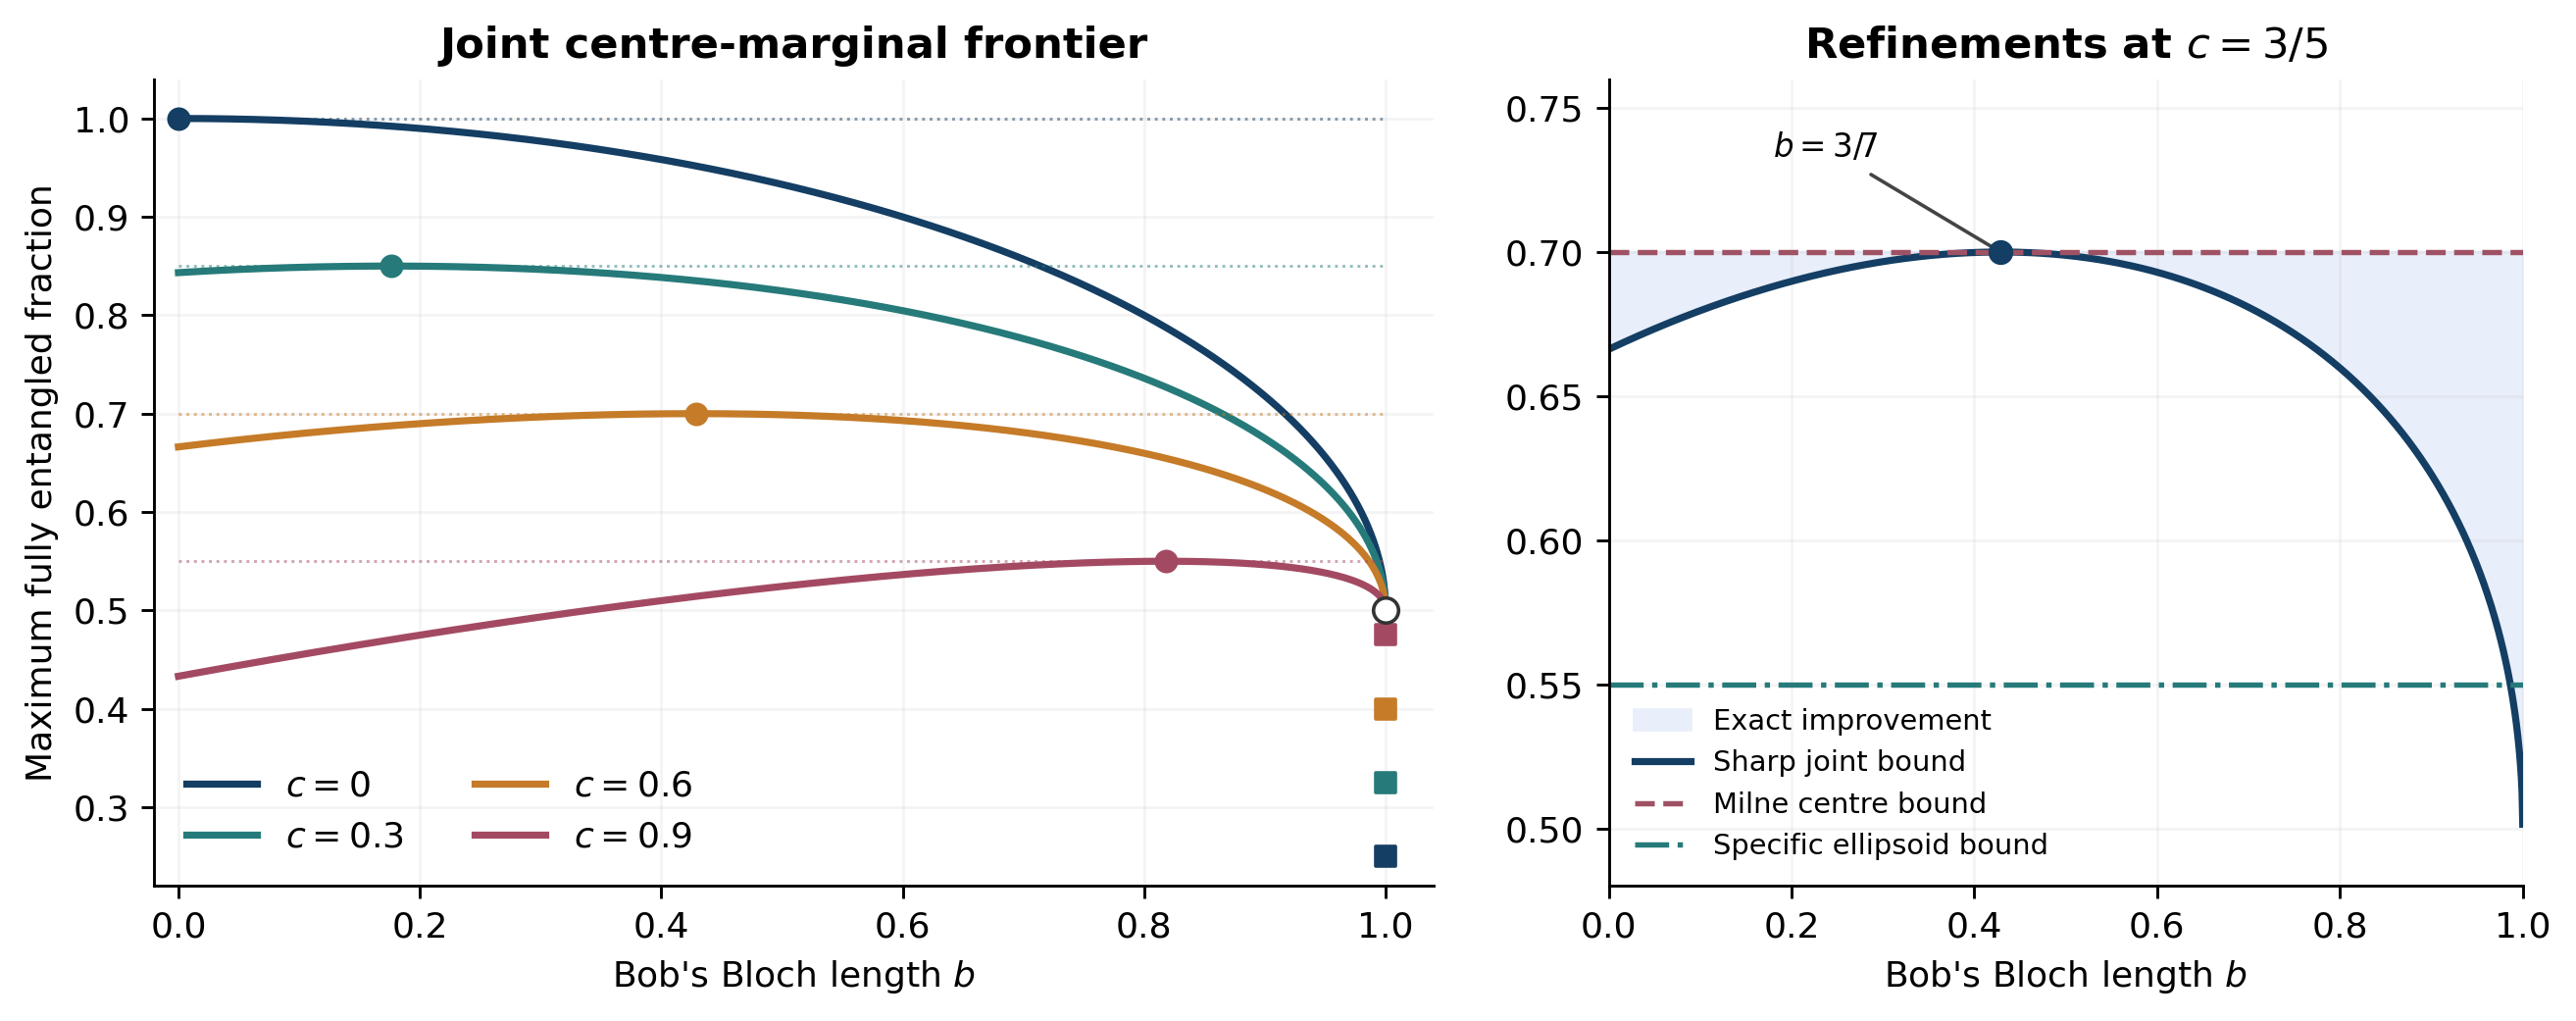
\includegraphics[width=\textwidth]{sharp_frontier.png}
\caption{Left: the exact frontier for $b<1$. Dots mark the centre-only maxima; squares give the distinct exact values on the singular $b=1$ stratum. The open endpoint marks the $b\to1^-$ limit. Right: joint and shape refinements at $c=3/5$; the shape line applies to the specific ellipsoid of Section~\ref{sec:shape}, not to every state with that centre.}
\end{figure}

The exact improvement over Milne's inequality is
\begin{equation}\label{eq:deficit}
 \boxed{1-\frac c2-\Fe(c,b)=
 \frac{\bigl[\sqrt{1-b}-\sqrt{(1-c)(1+b)}\bigr]^2}{4}.}
\end{equation}
Consequently $\Fe(c,b)\le1-c/2$, with equality if and only if
\begin{equation}\label{eq:boptimal}
 b=\frac{c}{2-c}.
\end{equation}
At $b=0$, \eqref{eq:joint} reduces to Milne's established canonical-state theorem
\[
 \Fe(c,0)=\frac{(1+\sqrt{1-c})^2}{4}.
\]
The joint theorem therefore interpolates two previously separate bounds, and proves a strict improvement whenever $b\ne c/(2-c)$.

If $\varepsilon=1-c/2-f(\rho)$, then
\begin{equation}\label{eq:qubit-stability}
 \left|b-\frac{c}{2-c}\right|^2\le\frac{8\varepsilon}{2-c}.
\end{equation}
One way to see this is the $d=2$ instance of \eqref{eq:highdim-stability}. Alternatively rationalize the difference in \eqref{eq:deficit} and use
\[
 \bigl[\sqrt{1-b}+\sqrt{(1-c)(1+b)}\bigr]^2\le2(2-c).
\]
The exact identity, unique value \eqref{eq:boptimal}, and inequality \eqref{eq:qubit-stability} are checked in Lean.


\subsection{The optimal fixed-centre stability coefficient}
The earlier estimate can be sharpened to its best possible coefficient, including the singular Bob stratum.

\begin{theorem}[Optimal quantitative marginal rigidity]\label{thm:optimal-stability}
For every two-qubit density matrix, let
\[
 \epsilon=1-c/2-f(\rho),\qquad b=|\bm b|,\qquad
 K(c)=4\bigl(1+\sqrt{1-c}\bigr)^2.
\]
Then
\begin{equation}\label{eq:optimal-stability}
 \boxed{\bigl((2-c)b-c\bigr)^2\le K(c)\epsilon,\qquad
 \left|b-\frac{c}{2-c}\right|^2
 \le\frac{4(1+\sqrt{1-c})^2}{(2-c)^2}\epsilon.}
\end{equation}
For each fixed $c\in[0,1]$, the coefficient $K(c)$ is the smallest possible coefficient in the first inequality over all states with that centre radius. For $c>0$ it is attained by the joint-frontier state with $b=0$. For $c=0$ it is approached by the frontier family as $b\downarrow0$.
\end{theorem}
\begin{proof}
The continuous expression $\Fe(c,b)$ remains an upper bound at $b=1$, because there it equals $1/2$ and the actual product-state FEF is $(1+c)/4\le1/2$. Thus $\epsilon\ge D(c,b):=1-c/2-\Fe(c,b)$ throughout the physical domain.
Put $u=\sqrt{1-b}$ and $v=\sqrt{1-c}\sqrt{1+b}$. The exact deficit identity gives
\[
 D(c,b)=\frac{(u-v)^2}{4},\qquad
 \bigl((2-c)b-c\bigr)^2=4(u+v)^2D(c,b).
\]
Since $c,b\ge0$,
\[
 (u+v)^2=2-c-cb+2\sqrt{1-c}\sqrt{1-b^2}
 \le2-c+2\sqrt{1-c}=(1+\sqrt{1-c})^2.
\]
This proves the bound. At $b=0$ and $c>0$, both inequalities used above are equalities for the explicit frontier state, and its deficit is strictly positive. Hence its ratio of squared displacement to deficit is exactly $K(c)$.
At $c=0$ and $0<b<1$, that ratio is
\[
 \frac{4b^2}{(1-\sqrt{1-b^2})/2}
       =8(1+\sqrt{1-b^2}),
\]
which approaches $16=K(0)$. No smaller coefficient can hold uniformly.
\end{proof}

The improvement over the earlier coefficient $8(2-c)$ is exactly
$4(1-\sqrt{1-c})^2$. The theorem controls the marginal radius. It is not a trace-distance estimate to a single state in higher dimensions, where the optimizer face can contain many states.

\section{Complete equality classification}\label{sec:equality}
\begin{theorem}[All joint-frontier maximizers]\label{thm:joint-equality}
For every $0\le c\le1$ and $0\le b<1$, a two-qubit state attains \eqref{eq:joint} if and only if it is locally unitarily equivalent to \eqref{eq:joint-state}.
\end{theorem}
\paragraph{Idea of the proof.} Equality must hold in every step of the
proof of Theorem~\ref{thm:weighted}. The extracted vector $w$ must then have
the largest admissible Schmidt coefficients, the positive residual
$\sigma-\ket w\bra w$ must live where the target cannot see it, and the filter
must be aligned with the Schmidt bases of $w$. Each of these conditions is
rigid, and together they determine the state up to local unitaries.

\begin{proof}
First assume $0<c<1$. Choose a maximizing maximally entangled $e$ and write the state as a filter of its canonical $\sigma$. Put $x=(\Id\otimes K^\dagger)e$, so $x$ is unit with Schmidt amplitudes
\[
 s_1=\sqrt{(1+b)/2},\qquad s_2=\sqrt{(1-b)/2}>0.
\]
Extract $w=\sigma x/\sqrt{t}$, $t=\bra x\sigma\ket x=\Fe(c,b)>0$. In the proof of Theorem~\ref{thm:weighted} every inequality must be an equality. Both positive $s_i$ force the squared Schmidt amplitudes of $w$ to be
\[
 q_1=\frac12,\qquad q_2=\frac{1-c}{2}.
\]
Apply local unitaries to put
\[
 w=\frac1{\sqrt2}\bigl(\ket{00}+\sqrt{1-c}\ket{11}\bigr),\qquad
 R=\sigma-\ket w\bra w\succeq0.
\]
The Bob marginal then satisfies
\[
 R_B=\frac c2\ket1\bra1.
\]
A positive operator with its Bob marginal supported on $\ket1$ is supported on $\C^2\otimes\mathrm{span}\{\ket1\}$: the expectation on every vector with Bob component $\ket0$ is zero, and a positive operator annihilates a vector of zero expectation. Hence $R=H\otimes\ket1\bra1$ with $H\succeq0$ and $\tr H=c/2$.

Now $\sigma_A=\diag(q_1,q_2)+H$ has smallest eigenvalue $q_2$. Take a unit eigenvector $u$ for that eigenvalue. The two nonnegative terms
\[
 \ip{u}{(\diag(q_1,q_2)-q_2\Id)u}\quad\text{and}\quad\ip{u}{Hu}
\]
sum to zero. Because $q_1>q_2$, $u$ is a phase multiple of $\ket1$, and positivity implies $H\ket1=0$. Therefore $H=(c/2)\ket0\bra0$. We have proved that the canonical state is exactly
\begin{equation}\label{eq:sigma-ad}
 \sigma_c=\frac12\bigl(\ket{00}+\sqrt{1-c}\ket{11}\bigr)
                    \bigl(\bra{00}+\sqrt{1-c}\bra{11}\bigr)
            +\frac c2\ket{01}\bra{01}.
\end{equation}

It remains to check the filter orientation, rather than merely its singular values. In the chosen Schmidt bases write $W=\diag(w_1,w_2)$ with $w_1>w_2>0$, and let $X$ be the coefficient matrix of $x$. Then
\[
 |\tr(W^\dagger X)|
 \le(w_1-w_2)|X_{00}|+w_2|\tr X|
 \le(w_1-w_2)s_1+w_2(s_1+s_2).
\]
Equality forces $|X_{00}|=s_1$. Since $s_1$ is the operator norm of $X$, the off-diagonal entries in its first row and column must vanish. The remaining diagonal entry has modulus $s_2$, and equality in the triangle inequality aligns the two phases. Thus, up to an irrelevant overall phase,
\[
 x=s_1\ket{00}+s_2\ket{11}.
\]
This argument also covers $b=0$, when $s_1=s_2$; only the strict inequality $w_1>w_2$ was used.

If $E$ is the coefficient matrix of the maximally entangled $e$, then $E^\dagger E=\Id/2$ and $X=E\overline K$. Consequently
\[
 K^\dagger K=2(X^\dagger X)^T=\diag(1+b,1-b).
\]
Polar decomposition absorbs the remaining output unitary into a local Bob unitary. Filtering \eqref{eq:sigma-ad} by this positive diagonal matrix's square root gives exactly \eqref{eq:joint-state}.

For $c=0$, equality in both positive-weight caps gives $\|w\|^2=1$. The positive residual has trace zero and vanishes, so $\sigma$ is a pure maximally entangled state. The filtered state is pure, and its Schmidt spectrum is fixed by $b$; all such pure states form one local-unitary orbit, represented by $\rho_{0,b}$.

For $c=1$, $\sigma_A$ is pure, so $\sigma=\ket0\bra0\otimes\Id/2$ up to local unitaries. The state $\rho$ is pure Alice tensor Bob, and all states with the given $b$ again form one local-unitary orbit. Their FEF is $(1+b)/4=\Fe(1,b)$. The converse in all cases follows from the explicitly checked attaining family.\end{proof}

\begin{corollary}[All saturators of Milne's original inequality]\label{cor:original-equality}
For each $c\in[0,1]$ there is exactly one local-unitary orbit of states satisfying $f(\rho)=1-c/2$. A representative is
\begin{equation}\label{eq:milne-saturator}
 \boxed{\rho_c=
 \frac{\ket{\chi_c}\bra{\chi_c}+c(1-c)\ket{01}\bra{01}}{2-c},
 \qquad\ket{\chi_c}=\ket{00}+(1-c)\ket{11}.}
\end{equation}
At $c=0$ these are exactly pure maximally entangled states; for $0<c<1$ they have rank two; at $c=1$ they are exactly pure product states. No full-rank state saturates.
\end{corollary}
\begin{proof}
For $b<1$, combine \eqref{eq:deficit} with Theorem~\ref{thm:joint-equality}: equality forces $b=c/(2-c)$ and substitution gives \eqref{eq:milne-saturator}. This includes $c=0$ and excludes $c=1$ within the full-rank Bob stratum.

For $b=1$, $\rho=\rho_A\otimes\ket\beta\bra\beta$. A direct Schmidt/Bell calculation gives
\begin{equation}\label{eq:singular}
 f(\rho)=\frac12\lambda_{\max}(\rho_A)=\frac{1+c}{4}.
\end{equation}
Equality with $1-c/2$ forces $c=1$, hence both marginals are pure.\end{proof}

\subsection{What happens at a singular Bob marginal}
For fixed $c<1$, $\lim_{b\to1^-}\Fe(c,b)=1/2$, whereas the exact value at $b=1$ is $(1+c)/4<1/2$. There is no discontinuity of the physical function $f(\rho)$: the matrices $\rho_{c,b}$ tend to the pure product $\ket{00}\bra{00}$, whose actual singular centre is $c=1$. It is the coordinate $c$ that fails to extend continuously along this approach. Replacing the singular branch by the limit would answer a different question.


\section{Sharp bounds from the full signed ellipsoid}\label{sec:shape}
\subsection{Exact filtering-orbit value}
For a canonical state $\sigma_B=\Id/d$ and any Bob filter $F\ne0$,
\[
 \rho_F=\frac{(\Id\otimes F)\sigma(\Id\otimes F^\dagger)}{\tr(F^\dagger F)/d}.
\]
For a maximally entangled $e$, let $x=(\Id\otimes F^\dagger)e$. Then
\[
 \bra e\rho_F\ket e=\frac{\bra x\sigma\ket x}{\|x\|^2}\le\lambda_{\max}(\sigma).
\]
Every coefficient matrix of a vector $x$ arises from some $F$ and a fixed Bell vector. Therefore
\begin{equation}\label{eq:orbit}
 \sup_{F\ \mathrm{invertible}}f_d(\rho_F)=\lambda_{\max}(\sigma).
\end{equation}
The supremum is an actual maximum among invertible filters if and only if the top eigenspace contains a full-Schmidt-rank vector. Otherwise singular filters attain the closed-orbit optimum and invertible filters approach it. Singular filtering can change the steering ellipsoid, so it must not be silently described as preserving the original ellipsoid.

For qubits this is equivalent, through the channel--state correspondence, to the established optimization of Pal, Bandyopadhyay and Ghosh \cite{pal}. It is useful here but not claimed as a new optimization theorem.

\subsection{An explicit polynomial in geometric invariants}
Write the canonical Bloch form as
\[
 \sigma=\frac14\left(\Id+\bm c\cdot\bm\sigma\otimes\Id+
 \sum_{ij}S_{ij}\sigma_i\otimes\sigma_j\right),\qquad Q=SS^T.
\]
Besides $c$, use
\[
 q=\tr Q,\quad q_2=\tr(Q^2),\quad k=\bm c^TQ\bm c,\quad
 d_S=\det S=\chi\sqrt{\det Q},\quad r=c^2+q.
\]
For $H=4\sigma-\Id$, the characteristic polynomial is
\begin{equation}\label{eq:quartic}
 \boxed{P_H(z)=z^4-2rz^2+8d_Sz+r^2-4k-2q^2+2q_2.}
\end{equation}
If $z_+$ is its largest root, then
\begin{equation}\label{eq:geometric-bound}
 f(\rho)\le\Lambda(\bm c,Q,\chi):=\frac{1+z_+}{4}\le1-\frac c2.
\end{equation}
This gives the exact filtering-orbit supremum, with the attainment condition above. Unlike the centre-only bound, it uses shape, skew and chirality.

To verify \eqref{eq:quartic}, local unitary rotations diagonalize $S$ by signed singular values, leaving an arbitrary $\bm c$. Direct Pauli multiplication gives
\begin{align*}
 \tr H&=0,&\tr H^2&=4r,&\tr H^3&=-24d_S,\\
 \tr H^4&=4r^2+16k+8(q^2-q_2).
\end{align*}
Newton identities give the polynomial. The supplied SymPy calculation verifies the determinant with all diagonal signed correlations and all three centre components symbolic; the numerical harness checks the invariant formula without diagonalizing $S$ first. Its determinant ancestry is already present in steering-ellipsoid physicality work \cite{milnegeometry}.

\textbf{Chirality matters.} An unsigned ellipsoid need not identify a unique canonical spectrum. At $c=0$, $Q=(1/16)\Id$, the physical states with $S=\diag(1/4,-1/4,1/4)$ and $S=\diag(1/4,1/4,1/4)$ have the same unsigned geometry but different orbit optima, $7/16$ and $5/16$. For an unsigned-only bound take the maximum over physically admissible chiralities. In the entangled qubit case the chirality is necessarily negative.

\subsection{Strict exact example}
Take
\[
 \bm c=(0,0,3/5),\qquad S=\diag(2/5,-2/5,1/5).
\]
Then $\spec\sigma=(11/20,7/20,1/20,1/20)$. Thus the best ellipsoid bound is $11/20$, versus the centre-only value $7/10$. Filtering Bob with $F=\diag(1,1/2)$ succeeds with probability $5/8$ and produces
\[
 \rho=\begin{pmatrix}
 18/25&0&0&4/25\\
 0&7/50&0&0\\
 0&0&2/25&0\\
 4/25&0&0&3/50
 \end{pmatrix},\qquad f(\rho)=11/20.
\]
This example proves the shape refinement is both strict and attainable. It also shows that the full-ellipsoid and joint-centre/marginal refinements carry different information; taking their minimum is valid.

For $0<c<1$, the centre-only envelope equals the ellipsoid envelope only for the maximally obese geometry
\[
 \bm c=c\bm e_z,\qquad Q=\diag(1-c,1-c,(1-c)^2),\qquad\chi=-1,
\]
up to rotations. Indeed equality in the canonical spectral bound forces \eqref{eq:sigma-ad}; conversely that state has top eigenvalue $1-c/2$ and a full-Schmidt-rank top eigenvector. The endpoint $c=1$ is a point ellipsoid, with a supremum approached through nearly singular Bob filters.


\section{A sharp bound from the centre and squared semiaxes}\label{sec:purity-envelope}
Let $\sigma$ be canonical, $\sigma_B=I/2$, with Alice Bloch-vector length $c$ and correlation matrix $S$. Put
\[
 Q=SS^T,\qquad q=\tr Q,\qquad P=\tr\sigma^2=\frac{1+c^2+q}{4}.
\]
Thus $q$ is the sum of the squared ellipsoid semiaxes. It requires neither their individual values nor the full signed geometry.

\begin{theorem}[Exact two-invariant envelope]\label{thm:purity-envelope}
The physically possible pairs are exactly
\[
 0\le c\le1,\qquad 0\le q\le3-4c+c^2.
\]
Among all canonical states with these invariants, the exact maximum of $\lambda_{\max}(\sigma)$ is $H(c,q)$ below.
For $0\le c\le2/3$, put $q_1=c^2/4$ and $q_2=3-6c+5c^2/2$. Then
\[
 \boxed{H(c,q)=
 \begin{cases}
 (1+c+\sqrt q)/4,&0\le q\le q_1,\\
 (1+\sqrt{3q+3c^2/2})/4,&q_1\le q\le q_2,\\
 (2-c+\sqrt{2q+4c-2-c^2})/4,&q_2\le q\le3-4c+c^2.
 \end{cases}}
\]
For $2/3\le c\le1$, the middle branch disappears:
\[
 \boxed{H(c,q)=
 \begin{cases}
 (1+c+\sqrt q)/4,&0\le q\le(1-c)^2,\\
 (2-c+\sqrt{2q+4c-2-c^2})/4,&(1-c)^2\le q\le3-4c+c^2.
 \end{cases}}
\]
Every state in the invertible Bob-filter orbit of $\sigma$ satisfies $f(\rho)\le H(c,q)$. This bound is sharp as a supremum for every allowed pair.
\end{theorem}

\subsection{Proof by exact quadratic certificates}
Write the ordered spectrum as $\lambda\ge u\ge v\ge w\ge0$, and put $h=c/2$. Bravyi's two-qubit marginal theorem~\cite{bravyi} gives
\begin{equation}\label{eq:bravyi-used}
 v+w\le\tfrac12-h,\qquad \lambda-v\ge h,\qquad u-w\ge h.
\end{equation}
The additional inequality $\lambda-w\ge h$ is redundant here. These established quantum-marginal constraints are an explicit dependency of the proof.

Trace one and the first inequality imply $\lambda\ge(1+c)/4$, while $u\ge h$ gives $\lambda\le1-h=:L$.
If $\lambda\le1/2$, then $P\le\lambda\le1/2\le L^2+(1-L)^2$.
If $\lambda\ge1/2$, then
$P\le\lambda^2+(1-\lambda)^2\le L^2+(1-L)^2$.
Hence $q\le3-4c+c^2$.

For fixed $\lambda,c$, the minimum possible purity is attained by these spectra:
\[
\begin{array}{c|c}
 \text{branch}&(\lambda,u,v,w)\\ \hline
 \mathrm I&(\lambda,\frac12-\lambda+h,\lambda-h,\frac12-\lambda)\\[2pt]
 \mathrm {II}&(\lambda,r+h/2,r,r-h/2),\quad r=(1-\lambda)/3\\[2pt]
 \mathrm {III}&(\lambda,h,1-\lambda-h,0).
\end{array}
\]
Their purities are
\begin{align*}
 P_{\mathrm I}&=\frac{1+c^2}{4}+4\left(\lambda-\frac{1+c}{4}\right)^2,\\
 P_{\mathrm {II}}&=\lambda^2+\frac{(1-\lambda)^2}{3}+\frac{c^2}{8},\\
 P_{\mathrm {III}}&=\lambda^2+h^2+(1-\lambda-h)^2.
\end{align*}
For $c\le2/3$, the branch intervals in $\lambda$ are
\[
 \left[\frac{1+c}{4},\frac{2+3c}{8}\right],\quad
 \left[\frac{2+3c}{8},1-\frac{3c}{4}\right],\quad
 \left[1-\frac{3c}{4},1-\frac c2\right].
\]
For $c\ge2/3$, branches I and III instead occupy
$[(1+c)/4,1/2]$ and $[1/2,1-c/2]$.

Here are direct certificates. If $(u_0,v_0,w_0)$ is the proposed remaining spectrum and $U=u-u_0,V=v-v_0,W=w-w_0$, then $U+V+W=0$ and
\[
 P-P_{\min}=U^2+V^2+W^2+2(u_0U+v_0V+w_0W).
\]
In branch I put $d=2\lambda-h-1/2$. The constraints imply $U\ge0$, $2U+V\ge0$, and $0\le d\le h/2$. The linear term is
\[
 u_0U+v_0V+w_0W=d(2U+V)+(h-2d)U\ge0.
\]
In branch II it is $(h/2)(U-W)\ge0$ by $u-w\ge h$.
In branch III put $v_0=1-\lambda-h$. Then $W=w\ge0$, $U-W\ge0$, and the linear term is
\[
 (h-v_0)(U-W)+(h-2v_0)W\ge0.
\]
Both coefficients are nonnegative on the stated interval. Each certificate is therefore a sum of squares and nonnegative multiples of spectral constraints. The proposed spectra satisfy ordering and all constraints. Their purities increase with $\lambda$, agree at the joins, and inversion gives $H$.

\subsection{Sharp states}
For each optimizing spectrum, $u-w=h$. Define
\[
 a=\frac{\lambda+v+h}{2},\qquad d=\frac{\lambda+v-h}{2},\qquad
 z=\frac{\sqrt{(\lambda-v)^2-h^2}}2,
\qquad
 \sigma=\begin{pmatrix}
 a&0&0&z\\0&u&0&0\\0&0&w&0\\z&0&0&d
 \end{pmatrix}.
\]
The correlated block has eigenvalues $\lambda,v$, the other eigenvalues are $u,w$, and the marginals are $\diag((1+c)/2,(1-c)/2)$ and $I/2$. This realizes every allowed pair and proves sharpness. No converse invocation of Bravyi is needed.

The supremum of FEF in a canonical state's invertible Bob-filter orbit is its top eigenvalue, as established in Section~\ref{sec:shape}. In the interiors of branches II and III, $z>0$ and the top eigenvector is entangled, so an invertible filter attains $H$. Product top eigenvectors can be approached by invertible filters, proving sharpness as a supremum elsewhere. Singular output limits require recomputing the ellipsoid; point ellipsoids can persist at such a limit.

\paragraph{An exact strict improvement.}
At $c=3/5,q=2/5$,
\[
 H(c,q)=\frac{7+\sqrt{21}}{20}\simeq0.57913<\frac7{10}.
\]
An attaining canonical state is
\[
 \sigma=\begin{pmatrix}
 1/2&0&0&\sqrt3/10\\
 0&3/10&0&0\\
 0&0&0&0\\
 \sqrt3/10&0&0&1/5
 \end{pmatrix}.
\]
For $b=3/\sqrt{21}$ and $K=\diag(\sqrt{1+b},\sqrt{1-b})$, the normalized state $(I\otimes K)\sigma(I\otimes K)$ has Bell overlap
\[
 \frac7{20}+\frac{3b}{20}+\frac{\sqrt3}{10}\sqrt{1-b^2}
       =\frac{7+\sqrt{21}}{20}.
\]
The filter preserves the ellipsoid, so this is actual FEF attainment.

\begin{figure}[htbp]\centering
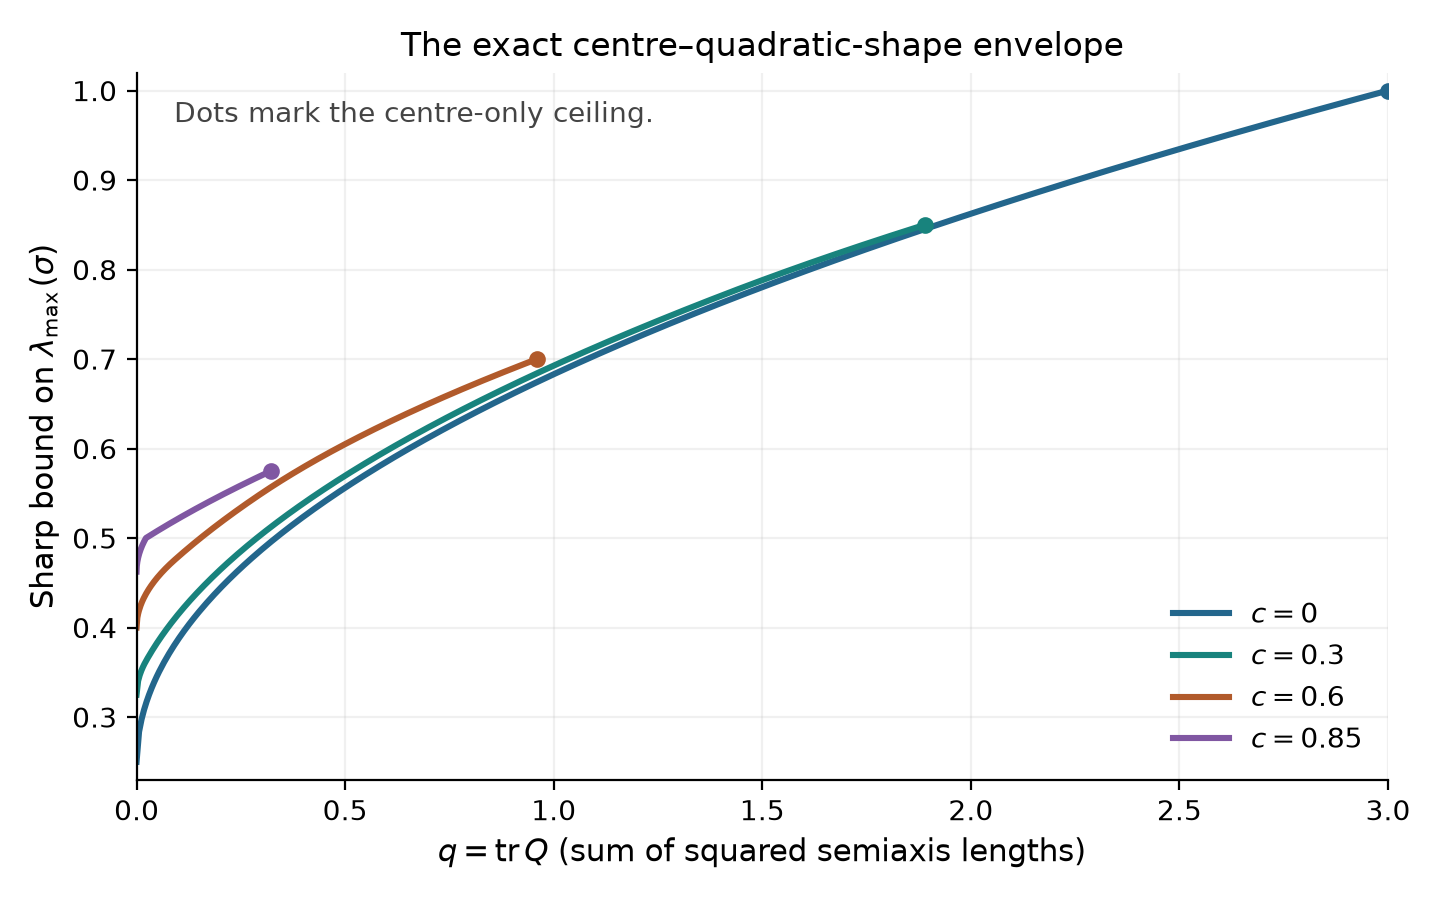
\includegraphics[width=.96\textwidth]{purity_envelope.png}
\caption{The exact two-invariant envelope. The analytic branches meet continuously; the centre-only bound is recovered at the largest allowed $q$. Curves evaluate the proved formulas.}
\end{figure}

\subsection{Complete low-branch equality and invertible-filter nonattainment}

\begin{theorem}[Classical rigidity of low-branch maximizers]\label{thm:low-branch}
Let $0<c\le1$ and $0\le q\le q_*(c):=\min\{c^2/4,(1-c)^2\}$. Put
\[
 \lambda=H(c,q)=\frac{1+c+\sqrt q}{4},\qquad h=c/2.
\]
Every canonical state with these invariants and largest eigenvalue $\lambda$ is, up to local unitaries, the single state
\begin{equation}\label{eq:low-classical}
 \sigma=\diag\left(\lambda,\frac12-\lambda+h,
                         \frac12-\lambda,\lambda-h\right).
\end{equation}
It is classical in a product basis, and every vector in its top eigenspace is a product vector. For every invertible Bob-filtered output of such a state, with actual Bob radius $b<1$,
\begin{equation}\label{eq:low-filtered}
 \boxed{f(\rho)\le H(c,q)-\frac{c(1-b)}4
                   =\frac{1+\sqrt q+cb}{4}<H(c,q).}
\end{equation}
For each fixed $b\in[0,1)$ equality in the first inequality is attained by a diagonal filter of~\eqref{eq:low-classical}.
Consequently, throughout the positive-$c$ low branch, the two-invariant bound is a strict supremum when Bob's marginal is required to remain invertible.
\end{theorem}
\begin{proof}
Equality in the minimum-purity certificate forces each squared deviation to vanish. Therefore the ordered spectrum is
\[
 (\lambda,u,v,w)=
 \left(\lambda,\frac12-\lambda+h,\lambda-h,\frac12-\lambda\right).
\]
Writing $d=2\lambda-h-1/2=\sqrt q/2$, one has $0\le d\le h/2$ and $u-v=h-d>0$. Let $a$ be the top eigenvector of the Alice marginal and put $P=|a\rangle\langle a|\otimes I$. This rank-two projection has
\[
 \tr(P\sigma)=\frac{1+c}{2}=\lambda+u.
\]
For completeness, in an orthonormal eigenbasis $e_i$ of $\sigma$, put $p_i=\langle e_i,Pe_i\rangle$. These numbers lie in $[0,1]$ and sum to two. The spectral gap gives
\[
 \lambda+u-\sum_i\lambda_i p_i\ge(u-v)(p_3+p_4).
\]
Thus $p_3=p_4=0$ and $p_1=p_2=1$. Projection positivity implies that $P$ is exactly the projection onto the top-two spectral subspace. Hence
\[
 \sigma=|a\rangle\langle a|\otimes R_0+
        |a^\perp\rangle\langle a^\perp|\otimes R_1,
 \qquad R_1=I/2-R_0.
\]
The two Bob blocks commute and can be simultaneously diagonalized, yielding~\eqref{eq:low-classical}. Its entire top eigenspace lies in $|a\rangle\otimes\C^2$.

Moreover $\sigma\preceq\lambda P+v(I-P)$. A normalized reverse-filtered maximally entangled test vector has squared Schmidt coefficients $(1+b)/2,(1-b)/2$, so its expectation in $P$ is at most $(1+b)/2$. Its expectation in $\sigma$ is therefore at most
\[
 \lambda\frac{1+b}{2}+v\frac{1-b}{2}
       =\lambda-\frac{c(1-b)}4.
\]
For the displayed diagonal state, the filter $K=\diag(\sqrt{1+b},\sqrt{1-b})$ and Bell vector $\Phi^+$ attain this value. This proves the exact filtered claim for the family of canonical low-branch extremizers. If any other state with the same $(c,q)$ attained $H$, its canonical state would also have top eigenvalue $H$, hence would belong to this family, contradicting the strict inequality.
\end{proof}

At $c=q=0$, the canonical state is $I/4$ and the envelope $1/4$ is attained. For $c>0$, the $b=1$ limit of~\eqref{eq:low-classical} is a point ellipsoid of centre length $c+\sqrt q$. For $q>0$ this changes the invariants. For $q=0$ the point ellipsoid is preserved and a singular product output attains $H(c,0)=(1+c)/4$. Formula~\eqref{eq:low-filtered} is an exact finite-bias result for canonical states that maximize $\lambda_{\max}$; it is not asserted to be the full three-invariant $(c,q,b)$ envelope for all states.

The underlying spectral compatibility inequalities are Bravyi's established theorem. The optimization, sharp realization, and low-branch equality analysis above are deductions checked by exact computation. The \texttt{PurityCertificates} section of \texttt{AllProofs.lean} addresses the three real quadratic certificates; it does not install Bravyi's theorem as an axiom or claim an end-to-end formalization of this ellipsoid result.

\section{An exact reduction for arbitrary fixed marginal matrices}\label{sec:reduction}
The spectral formula does not directly solve the problem of a prescribed target that is misaligned with prescribed marginal matrices. An exact variational reduction does. It is valid in rectangular dimensions and for singular marginals.

Let $A$ and $B$ be density matrices on $\C^m$ and $\C^n$, and let $x=\operatorname{vec}X\in\C^m\otimes\C^n$ be a unit vector, using row-major coefficients $X_{ij}$ in $\ket{i}\otimes\ket{j}$. Then the marginals of $ww^\dagger$, for $w=\operatorname{vec}W$, are $WW^\dagger$ and $(W^\dagger W)^T$.

\begin{theorem}[Exact pure-component variational reduction]\label{thm:reduction}
Define
\[
 \mathcal W(A,B)=\{W\in\C^{m\times n}:WW^\dagger\preceq A,\ W^\dagger W\preceq B^T\}.
\]
Then
\begin{equation}\label{eq:reduction}
 \boxed{\max_{\rho_A=A,\,\rho_B=B}\bra x\rho\ket x
 =\left[\max_{W\in\mathcal W(A,B)}\Rea\tr(X^\dagger W)\right]^2
 =\left[\max_{W\in\mathcal W(A,B)}|\tr(X^\dagger W)|\right]^2.}
\end{equation}
Both maxima are attained. An optimal $W$ produces an actual optimal density matrix by a rank-one term plus a separable product residual.
\end{theorem}
\begin{proof}
If $t=\bra x\rho\ket x>0$, rank-one extraction gives $w=\rho x/\sqrt t$, $\rho\succeq ww^\dagger$ and $\langle x,w\rangle=\sqrt t$. Taking partial traces gives the two constraints on its coefficient matrix. If $t=0$, use $w=0$. This proves one inequality.

Conversely, for any feasible $W$ put $w=\operatorname{vec}W$,
\[
 A_0=A-WW^\dagger,\quad B_0=B-(W^\dagger W)^T,\quad
 \delta=\tr A_0=\tr B_0=1-\|w\|^2.
\]
When $\delta>0$,
\begin{equation}\label{eq:completion}
 \rho_W=ww^\dagger+\frac{A_0\otimes B_0}{\delta}
\end{equation}
is positive, has trace one and the required actual marginals. Its target overlap is at least $|\langle x,w\rangle|^2$. When $\delta=0$, positivity forces $A_0=B_0=0$, and $ww^\dagger$ alone is a coupling. This proves the opposite inequality. The feasible vector set is closed and bounded by $\|w\|^2\le1$, and the coupling set is compact and nonempty, so maxima exist. Finally global phase preserves the constraints on $W$ and rotates its overlap to a nonnegative real number. At a maximizing $W$, the completion must have exactly the optimal overlap; any extra positive residual contribution would contradict the already-proved equality.
\end{proof}

The positive completion formula itself has a general prior antecedent in
Remark 2.4(ii) of Skalski--Todorov--Turowska~\cite{capacity2025}.
The reduction additionally extracts a rank-one component from an arbitrary
coupling and identifies the exact target optimization, including optimizer
transfers.

\subsection{A smaller semidefinite optimization problem}
The feasible set $\mathcal W(A,B)$ is convex. By the Schur complement its constraints are equivalent to
\[
 \begin{pmatrix}A&W\\W^\dagger&\Id_n\end{pmatrix}\succeq0,
 \qquad
 \begin{pmatrix}\Id_m&W\\W^\dagger&B^T\end{pmatrix}\succeq0.
\]
Thus maximizing the real amplitude is a semidefinite program with $2mn$ real scalar variables and two positive blocks of size $m+n$. Squaring its nonnegative optimum gives the original optimum over a positive matrix of size $mn$, which has $(mn)^2$ real entries before constraints. This is an exact size reduction, not a relaxation. The numerical checks compare both formulations for independently generated, misaligned complex marginals and targets. Numerical solver tolerances are reported separately from exact proofs.

\begin{theorem}[Complementarity and a sharp optimizer-rank bound]\label{thm:rank-bound}
If $x$ has Schmidt rank $k\ge1$, some coupling maximizing its overlap has rank at most
\[
 \boxed{m+n-k.}
\]
It can be chosen as one pure positive term plus a separable residual. For a full-Schmidt target on $\C^d\otimes\C^d$, the bound becomes $d$ and is sharp even when both prescribed marginals are positive definite.
\end{theorem}
\begin{proof}
Take an optimal $W$ from Theorem~\ref{thm:reduction}. If $\delta=0$, the coupling is pure and the conclusion is immediate. Otherwise the nonnegative residual contribution in~\eqref{eq:completion} must vanish:
\[
 \bra x A_0\otimes B_0\ket x=0.
\]
The product is strictly positive on the product of its support spaces, so $x$ is orthogonal to that entire product support. Write $r=\rank A_0$ and $s=\rank B_0$. In coefficient-matrix language, $P_{A_0}X P_{B_0}^T=0$. The rank of $X$ restricted to the $s$-dimensional support of $B_0^T$ is at least $s-(n-k)$, while its image lies in a space of dimension $m-r$. Therefore
\[
 r+s\le m+n-k.
\]
In eigenbases of $A_0$ and $B_0$, couple their positive eigenvalues by a classical transportation matrix. The elementary greedy procedure matches two remaining positive masses, removes the smaller, and repeats. Each occupied cell exhausts at least one row or column, and the last exhausts both; hence it uses at most $r+s-1$ cells. The corresponding mixture of orthogonal product projectors has the same residual marginals, is supported on the same product space, and has rank at most $r+s-1$. It remains invisible to the target. Adding $ww^\dagger$ gives an optimal state of rank at most $r+s\le m+n-k$.

For $d=1$ the sharp rank is trivially one. For sharpness in the square case $d\ge2$, take $0<\eta<1/d$,
\[
 B=\Id/d,\qquad
 A=\diag\bigl(1/d+(d-1)\eta,\,1/d-\eta,\ldots,1/d-\eta\bigr),
\]
and any full-Schmidt positive diagonal target. The optimizer classification in Theorem~\ref{thm:optimizer-face} has one surplus Alice index and $d-1$ surplus Bob indices. It is unique, and its residual has rank $d-1$. The full optimizer therefore has rank exactly $d$. Both $A$ and $B$ are positive definite.
\end{proof}

The general extreme-point rank bound for fixed-marginal couplings is
$\rank\rho\le\sqrt{m^2+n^2-1}$, established by Parthasarathy~\cite{parthasarathy2003}. The target-dependent bound above can be combined with it by taking the smaller integer bound; it is not claimed to improve it for every target rank. For full-Schmidt square targets it improves the general bound to the sharp value $d$.

Klyachko's Theorem~6.4.1 already gives a coupling of prescribed marginals with rank at most the larger marginal rank, even while maximizing the spectral norm~\cite{klyachko}. Thus bare existence of a rank-$d$ coupling is established prior art. The conclusion here additionally optimizes an independently specified pure target. Applying Klyachko's theorem to $A_0,B_0$ gives the further credited existence refinement $\rank\rho\le1+\max(r,s)$; the Fourier construction below can make that residual separable. Target orthogonality of the entire residual product support preserves optimality. A further maximal-norm argument, given below, removes the extra one and establishes the stronger fixed-target bound $\max(m,n)$.

\paragraph{Subnormalized vectors are essential.}
Take $A=\diag(7/10,3/10)$, $B=\diag(3/10,7/10)$ and $x=\ket{\Phi^+}$. Every normalized pure coupling is
$\sqrt{7/10}\ket{01}+e^{i\theta}\sqrt{3/10}\ket{10}$ up to an overall phase, and has zero overlap with $x$. Nevertheless the unique optimal mixed coupling is
\[
 \rho_* =\frac3{10}(\ket{00}+\ket{11})(\bra{00}+\bra{11})
            +\frac25\ket{01}\bra{01},
 \qquad \bra x\rho_*\ket x=\frac35.
\]
Both marginals are positive and isospectral. The correct reduced optimizer has squared norm $3/5$, with its missing trace supplied by the residual. Restricting~\eqref{eq:reduction} to normalized pure couplings would therefore give a false answer.

% This standalone fragment does not overwrite the unique-core discussion.
\section{A sharp rank bound for every pure-target optimizer}
\label{sec:all-optimizer-rank}

The existence of a low-rank optimizer does not constrain the rank of other
points in an optimal face. The following theorem supplies a sharp bound for
every optimizer, including singular prescribed marginals.

For positive integers $m,n$ and $1\le k\le\min(m,n)$ define
\[
 N=m+n-k,\qquad
 R_{m,n,k}=\max\{rs:0\le r\le m,\ 0\le s\le n,\ r+s\le N,
                  \ r,s\text{ integers}\}.
\]
The elementary closed form is
\[
 R_{m,n,k}=
 \begin{cases}
 n(m-k),&m-n\ge k,\\
 m(n-k),&n-m\ge k,\\
 \lfloor(m+n-k)^2/4\rfloor,&|m-n|\le k.
 \end{cases}
\]
The formulas coincide at their shared boundaries.

\begin{theorem}[Sharp rank bound for all optimizers]
\label{thm:all-optimizer-rank}
Fix arbitrary density matrices $A,B$ on $\mathbb C^m,\mathbb C^n$ and a
unit pure target $x$ of Schmidt rank $k$. Every coupling maximizing
$\langle x,\rho x\rangle$ with these actual marginals obeys
\[
                  \boxed{\operatorname{rank}\rho\le1+R_{m,n,k}.}
\]
If the optimal target overlap is zero, the stronger bound
$\operatorname{rank}\rho\le R_{m,n,k}$ holds. No positivity assumption
on the marginal eigenvalues is needed.

For every specified unit target of Schmidt rank $k$, except the trivial
$m=n=k=1$ case, there exist positive definite marginals and an optimizer
of rank exactly $1+R_{m,n,k}$. Thus the universal bound is sharp for every
target Schmidt spectrum, not merely for one conveniently chosen target.
In square dimensions it reads
\[
 \boxed{\operatorname{rank}\rho\le
       1+\left\lfloor{(2d-k)^2\over4}\right\rfloor.}
\]
For a full-Schmidt target this is $1+\lfloor d^2/4\rfloor$.
\end{theorem}

\begin{proof}
Let $t=\langle x,\rho x\rangle$ be the optimal value. Suppose first that
$t>0$. The exact extraction
\[
 w={\rho x\over\sqrt t},\qquad R=\rho-ww^\dagger\ge0
\]
satisfies $\langle x,w\rangle=\sqrt t$ and $Rx=0$. Its residual
marginals are
\[
 A_0=A-\operatorname{Tr}_B(ww^\dagger),\qquad
 B_0=B-\operatorname{Tr}_A(ww^\dagger).
\]
They have the same nonnegative trace $\delta$. If $\delta=0$, $R=0$ and
$\rho$ is pure. Otherwise
$ww^\dagger+(A_0\otimes B_0)/\delta$ is another actual coupling.
Its overlap cannot exceed $t$, while its pure term already has overlap
$t$. Consequently
\[
                     \langle x,A_0\otimes B_0\,x\rangle=0.
\]
The product is positive definite on its support, so
$x\perp\operatorname{ran}A_0\otimes\operatorname{ran}B_0$.

Put $r=\operatorname{rank}A_0$ and $s=\operatorname{rank}B_0$.
In local bases adapted to these supports, the coefficient matrix $X$ of
$x$ has a zero $r\times s$ block. Splitting its rows and columns around
that block gives
\[
                k=\operatorname{rank}X\le(m-r)+(n-s),
                \qquad r+s\le N.
\]
Every positive matrix with residual marginals $A_0,B_0$ is supported on
their product support, so $\operatorname{rank}R\le rs$.
Since $Rx=0$ whereas $\langle x,w\rangle\ne0$, the vector $w$ is not in
$\operatorname{ran}R$. For a sum of positive matrices the range is the
sum of their ranges. Thus the ranks add exactly:
\[
        \operatorname{rank}\rho=1+\operatorname{rank}R
                             \le1+rs\le1+R_{m,n,k}.
\]

If $t=0$, the product coupling $A\otimes B$ must also have zero target
overlap. Hence $x\perp\operatorname{ran}A\otimes\operatorname{ran}B$.
Writing $r=\operatorname{rank}A$, $s=\operatorname{rank}B$, the same
zero-block argument gives $r+s\le N$. Every feasible coupling is
supported on that product space, so its rank is at most $rs\le R_{m,n,k}$.

To evaluate $R_{m,n,k}$, increasing either non-saturated variable cannot
decrease $rs$. An optimum may therefore be chosen with $r+s=N$.
Then $m-k\le r\le m$ and one maximizes the concave quadratic
$r(N-r)$ over this integer interval. The closest permitted integer to
$N/2$ gives the displayed piecewise formula.
\end{proof}

\begin{proof}[Sharpness construction]
Choose maximizing integers $r,s$ with $r+s=N$ and put
$a=m-r$, $b=n-s$. Then $a+b=k$. Outside the trivial one-dimensional
case, $r,s>0$. Write a Schmidt decomposition
\[
 x=\sum_{j=1}^{k}\sqrt{p_j}\,e_j\otimes f_j,
 \qquad p_j>0,\quad\sum_jp_j=1.
\]
Let $U$ contain the first $b$ Schmidt vectors on Alice and all of Alice's
unused Schmidt directions. Let $V$ contain the last $a$ Schmidt vectors
on Bob and all of Bob's unused Schmidt directions. Then
\[
 \dim U=b+(m-k)=r,\qquad \dim V=a+(n-k)=s,
\]
and
\[
 x\in(U\otimes V^\perp)\oplus(U^\perp\otimes V),
 \qquad x\perp U\otimes V.
\]
For any $0<q<1$ define
\[
 \rho_q=q\,xx^\dagger+{1-q\over rs}\,P_U\otimes P_V.
\]
It has rank $1+rs$. Both marginals are positive definite: the residual
is strictly positive on $U$ and $V$, while the target's nonzero Schmidt
coefficients cover their respective complements.

The local-sum operator
\[
          D=P_{U^\perp}\otimes I+I\otimes P_{V^\perp}
\]
is zero on $U\otimes V$, the identity on the two off-diagonal blocks
containing $x$, and twice the identity on
$U^\perp\otimes V^\perp$. Therefore $D\ge xx^\dagger$ and
$\operatorname{Tr}(D\rho_q)=q$. Every state with the same two marginals
has this same local-sum expectation and hence target overlap at most
$q$. The displayed state has target overlap exactly $q$, so it is an
optimizer attaining the bound. When $m=n=k=1$, the only coupling has
rank one, as claimed.
\end{proof}

\paragraph{Relation to prior rank bounds.}
Parthasarathy's general extremal-coupling bound is
$\operatorname{rank}\rho\le\sqrt{m^2+n^2-1}$
(arXiv:quant-ph/0307182). That is a statement about extreme points of the
whole coupling set. The theorem above instead concerns every point of
the exposed face selected by a pure target and tracks the target's Schmidt
rank. It complements the separate existence theorem giving an optimizer
of rank at most $\max\{\operatorname{rank}A,\operatorname{rank}B\}$. A high-rank member of the optimal face need not
be extreme. These distinctions are essential when comparing the bounds.
The precise target-dependent sharp theorem was not located in the bounded
primary-source search; historical priority has not been certified.

\paragraph{Verification scope.}
The proof is exact. The supporting rank-one extraction, positive completion,
and zero-residual-expectation steps are supplied in the finite-matrix Lean
modules. The full support/rank theorem is not claimed to be Lean formalized.
The accompanying exact-arithmetic script verifies the maximizing integer
formula, the sharp states and their local-sum dual certificates for small
rectangular dimensions and all allowed Schmidt ranks.

\subsection{What the two rank statements say in small dimensions}
For full-Schmidt targets on square systems, the existence bound and the
all-optimizer bound are both sharp, but answer different questions.
\begin{center}
\begin{tabular}{ccl}\toprule
Local dimension $d$ & Some optimizer & Every optimizer\\\midrule
2 & rank at most 2 & rank at most 2\\
3 & rank at most 3 & rank at most 3\\
4 & rank at most 4 & rank at most 5\\
5 & rank at most 5 & rank at most 7\\
6 & rank at most 6 & rank at most 10\\
8 & rank at most 8 & rank at most 17\\\bottomrule
\end{tabular}
\end{center}
For positive definite marginals, fixed full-Schmidt targets in dimensions
two and three have a unique optimizer, by the unique-core theorem below.
Dimension four permits both a nine-dimensional optimal face and rank-five
optimizers. Thus a low-rank attaining representative must not be mistaken
for a classification of all attaining states.

\section{A sharp low-rank optimizer with a separable remainder}
\label{sec:low-rank-optimizer}

The preceding rank bound controls every point of the optimal face. A stronger
existence statement holds independently of the target's Schmidt rank. It also
controls the form of an attaining ensemble.

\begin{theorem}[A low-rank pure-target optimizer]
\label{thm:low-rank-pure-target}
Let $A,B$ be arbitrary finite-dimensional density matrices, let $x$ be any
vector in their bipartite space, and put
\[
                 D=\max\{\operatorname{rank}A,\operatorname{rank}B\}.
\]
Among the states with actual marginals $A,B$, the maximum of
$\langle x,\rho x\rangle$ is attained by a state of the form
\[
 \boxed{\quad
 \rho=ww^\dagger+\sum_{j=1}^{q}p_j
                 |a_j\otimes b_j\rangle\langle a_j\otimes b_j|,
 \qquad 0\le q\le D-1,\quad p_j\ge0,
 \quad}
\]
where the local vectors $a_j,b_j$ are unit vectors. Consequently
\[
                         \boxed{\operatorname{rank}\rho\le D.}
\]
The pure core is subnormalized: $\|w\|^2+\sum_jp_j=1$.
The theorem includes singular marginals, rectangular systems, and the case
in which the optimal target overlap is zero. If the remainder is nonzero,
its product vectors can be chosen with equal weights $p_j=\delta/q$.
\end{theorem}

We first give the elementary coupling construction used in the proof.

\begin{lemma}[A short separable coupling of arbitrary marginals]
\label{lem:fourier-separable-coupling}
Suppose $E,F\ge0$ have the same positive trace $\delta$, and let
$q=\max\{\operatorname{rank}E,\operatorname{rank}F\}$. There is a
positive separable operator $R$ with marginals $E,F$ that is a sum of $q$
product projectors, and therefore has rank at most $q$. No separable
coupling with these marginals can have fewer than $q$ nonzero product
terms.
\end{lemma}

\begin{proof}
Diagonalize the marginals and pad their positive eigenvalue lists with zeros
to length $q$:
\[
 E=\sum_{i=0}^{q-1}a_i|e_i\rangle\langle e_i|,
 \qquad F=\sum_{j=0}^{q-1}b_j|f_j\rangle\langle f_j|,
 \qquad \sum_i a_i=\sum_jb_j=\delta.
\]
Terms with zero coefficients are omitted if the corresponding physical
space has dimension less than $q$. Write $\omega=e^{2\pi i/q}$ and define
\[
 u_t=\sum_i\sqrt{a_i}\,\omega^{ti}e_i,
 \qquad v_t=\sum_j\sqrt{b_j}\,\omega^{-tj}f_j,
 \qquad t=0,\ldots,q-1.
\]
Both vectors have squared norm $\delta$. Finite Fourier orthogonality gives
\[
 {1\over q}\sum_tu_tu_t^\dagger=E,
 \qquad {1\over q}\sum_tv_tv_t^\dagger=F.
\]
Hence
\[
 R={1\over q\delta}\sum_{t=0}^{q-1}
       (u_tu_t^\dagger)\otimes(v_tv_t^\dagger)
   ={\delta\over q}\sum_{t=0}^{q-1}
       \left|{u_t\over\sqrt\delta}\otimes
                    {v_t\over\sqrt\delta}\right\rangle
       \left\langle{u_t\over\sqrt\delta}\otimes
                    {v_t\over\sqrt\delta}\right|
\]
has the required marginals and is explicitly separable with $q$ terms.
Conversely, each product projector contributes rank at most one to each
marginal, so any separable ensemble requires at least
$\max\{\operatorname{rank}E,\operatorname{rank}F\}$ terms.

For comparison with a cyclic-matching construction, define
\[
 z_\ell=\sum_{i=0}^{q-1}
       \sqrt{a_i b_{i+\ell}/\delta}\;e_i\otimes f_{i+\ell},
       \qquad \ell=0,\ldots,q-1,
\]
with indices modulo $q$. The same Fourier identity gives
$R=\sum_\ell z_\ell z_\ell^\dagger$: both sides have entry
$\sqrt{a_i b_j a_k b_l}/\delta$ precisely when
$j-i=l-k\pmod q$, and entry zero otherwise. Individual $z_\ell$ may be
entangled; their sum of projectors nevertheless has the displayed
separable decomposition. Its rank is exactly $q$, because the $q$
nonzero matching vectors have disjoint supports when one eigenvalue
list has $q$ positive entries.
\end{proof}

\begin{proof}[Proof of Theorem~\ref{thm:low-rank-pure-target}]
Every feasible state is supported on
$\operatorname{ran}A\otimes\operatorname{ran}B$. Compress to these
supports and compress $x$ accordingly. Write their dimensions as $m,n$;
then $D=\max(m,n)$. The compressed target need not be a unit vector and
may vanish. The proof below allows both possibilities.

Use the coefficient-matrix convention
$w=\sum_{ij}W_{ij}|i,j\rangle$, so the pure marginal matrices are
$WW^\dagger$ and $(W^\dagger W)^T$. Set $C=B^T$ and consider
\[
 \mathcal K=\{W:\ WW^\dagger\le A,\quad W^\dagger W\le C\}.
\]
This is a nonempty compact set: it contains zero, is closed, and every
element obeys $\|W\|_F^2\le1$. It is convex, for example by the two
equivalent Schur-complement linear matrix inequalities. If $X$ is the
coefficient matrix of the compressed target, define
\[
 \tau=\max_{W\in\mathcal K}\operatorname{Re}\operatorname{Tr}(X^\dagger W).
\]
Phase invariance of $\mathcal K$ shows that this is also
$\max_{W\in\mathcal K}|\operatorname{Tr}(X^\dagger W)|$, and the exact
pure-target reduction identifies the optimal state overlap as $\tau^2$.
For completeness, the two directions of that reduction are the
rank-one extraction $w=\rho x/\sqrt{\langle x,\rho x\rangle}$ when the
denominator is nonzero, and the product-residual completion of any
feasible $w$. A zero state overlap uses $w=0$ instead. These arguments
do not require an invertible target or an invertible coupling.

Among all maximizers of the real linear objective, choose $W$ maximizing
$\|W\|_F^2$. Such a choice exists because the maximizing set is compact.
Put
\[
 E=A-WW^\dagger,\qquad F=C-W^\dagger W,
 \qquad \delta=\operatorname{Tr}E=\operatorname{Tr}F=1-\|W\|_F^2.
\]
If $\delta=0$, both residual matrices vanish, so $ww^\dagger$ is already
an optimal state of rank one. Suppose henceforth that $\delta>0$.

We claim
\[
                 \max\{\operatorname{rank}E,\operatorname{rank}F\}
                    \le D-1.                                      \tag{LR1}
\]
First assume $m\ge n$. If $E$ were positive definite, let
$V=\operatorname{ran}F$, of dimension $s\ge1$. Since
\[
                 \dim W(V^\perp)\le n-s<m,
\]
there is a nonzero vector $u\perp W(V^\perp)$. Choose any nonzero
$v\in V$ and set $Y=uv^\dagger$. Then $W^\dagger u\in V$, so all
three matrices
$W^\dagger Y$, $Y^\dagger W$, and $Y^\dagger Y$ are supported on $V$.
For sufficiently small $\varepsilon>0$, both signs satisfy
\[
 \begin{split}
 A-(W\pm\varepsilon Y)(W\pm\varepsilon Y)^\dagger
    &=E\mp\varepsilon(WY^\dagger+YW^\dagger)
                           -\varepsilon^2YY^\dagger\ge0,\\
 C-(W\pm\varepsilon Y)^\dagger(W\pm\varepsilon Y)
    &=F\mp\varepsilon(W^\dagger Y+Y^\dagger W)
                           -\varepsilon^2Y^\dagger Y\ge0.
 \end{split}
\]
The first assertion follows from strict positivity of $E$ on its full
space. The second follows from strict positivity of $F$ on $V$, since
the perturbations vanish on $V^\perp$ and have no cross blocks. Thus
both $W+\varepsilon Y$ and $W-\varepsilon Y$ lie in $\mathcal K$.
Their linear objectives average to the optimal value, so both are
themselves maximizers. But
\[
 {\|W+\varepsilon Y\|_F^2+\|W-\varepsilon Y\|_F^2\over2}
       =\|W\|_F^2+\varepsilon^2\|Y\|_F^2>\|W\|_F^2,
\]
contradicting the choice of $W$. Therefore
$\operatorname{rank}E\le m-1$. If $m>n$, also
$\operatorname{rank}F\le n\le m-1$. If $m=n$, apply the same argument
to $W^\dagger$ with the two caps exchanged to obtain
$\operatorname{rank}F\le n-1$. The case $n>m$ is symmetric. This proves
(LR1).

The product completion
\[
                ww^\dagger+{E\otimes F^T\over\delta}
\]
has marginals $A,B$. Its pure term already has target overlap $\tau^2$,
the global optimum. Consequently
\[
       \langle x,E\otimes F^T\,x\rangle=0,
       \qquad
       x\perp\operatorname{ran}E\otimes\operatorname{ran}F^T.       \tag{LR2}
\]
Here the second conclusion follows because the positive product matrix
is strictly positive on its support. The argument remains valid for
$\tau=0$: the product completion cannot have positive target overlap
when zero is the global maximum.

Apply Lemma~\ref{lem:fourier-separable-coupling} to $E,F^T$. It gives a
separable residual $R$ with these actual marginals and at most
$q=\max(\operatorname{rank}E,\operatorname{rank}F)\le D-1$ product
terms. It is supported on the space in (LR2), hence
$\langle x,Rx\rangle=0$. Therefore $\rho=ww^\dagger+R$ has the correct
actual marginals and still attains the global target optimum. Its rank
is at most $1+q\le D$, with the asserted separable decomposition.
\end{proof}

\paragraph{Sharpness in every rectangular dimension.}
The bound $D$ cannot be lowered, even for positive definite marginals.
Suppose $m\ge n$, let $A=I_m/m$, and choose a positive definite $B$ with
an eigenvalue $\beta>(m-1)/m$ and unit eigenvector $b$. For any coupling,
the positive principal block
$T=(I\otimes\langle b|)\rho(I\otimes|b\rangle)$ satisfies
$0\le T\le A$ and $\operatorname{Tr}T=\beta$. Consequently
\[
       \beta\le {\operatorname{rank}T\over m}
             \le {\operatorname{rank}\rho\over m},
       \qquad \operatorname{rank}\rho\ge m.
\]
Such $B$ exists for every $n$: for $n>1$, take the remaining eigenvalues
equal to $\varepsilon$ with
$0<\varepsilon<1/[m(n-1)]$; for $n=1$, take $B=[1]$. The case $n>m$
is symmetric. This example forces rank $D$ for every coupling, and
therefore makes the theorem sharp for every choice of target.

An explicit unique optimizer of rank $m$ is also available for a
maximal-Schmidt-rank target in every $m\ge n$ with $m>1$. Let
$0<\delta<1$, $\mu=(1-\delta)/n$, and
\[
 x={1\over\sqrt n}\sum_{i=0}^{n-1}|i,i\rangle,
 \quad w=\sqrt\mu\sum_{i=0}^{n-1}|i,i\rangle,
 \quad E={\delta\over m-1}\sum_{i=1}^{m-1}|i\rangle\langle i|.
\]
Take
\[
 A=\mu\sum_{i=0}^{n-1}|i\rangle\langle i|+E,
 \qquad B=\mu I_n+\delta|0\rangle\langle0|,
 \qquad \rho=ww^\dagger+E\otimes|0\rangle\langle0|.
\]
Both actual marginals are positive definite. Each target-diagonal
population is capped by $\mu$, so positivity and Cauchy--Schwarz give
target overlap at most $n\mu=1-\delta$, attained by this $\rho$.
For $n>1$, equality forces every target population to equal $\mu$ and
the target-diagonal principal block to be $ww^\dagger$. All remaining
nonzero populations are confined to
$\operatorname{span}\{|i,0\rangle:i\ne0\}$. Positivity therefore
writes any optimizer as
$ww^\dagger+wy^\dagger+yw^\dagger+R$ on these two blocks.
The off-diagonal Alice marginal entries with index zero force $y=0$;
the Alice marginal then forces $R=E\otimes|0\rangle\langle0|$.
Thus the displayed state is the unique optimizer and has rank $m$.
For $n=1$, the only coupling is $A\otimes B$, also of rank $m$.
For $m=n=1$, the only state has rank one.

\begin{corollary}[Fully entangled fraction and other target orbits]
For fixed actual marginals $A,B$ on $\mathbb C^d\otimes\mathbb C^d$,
the largest possible fully entangled fraction is attained by a state of
rank at most $D=\max(\operatorname{rank}A,\operatorname{rank}B)$, with
one pure core and at most $D-1$ product residual terms. The same holds
when the maximally entangled targets are replaced by any compact family
of pure targets, including a local-unitary orbit with prescribed Schmidt
coefficients.
\end{corollary}

\begin{proof}
The coupling set and the target family are compact, so choose a joint
maximizer $(\rho_*,x_*)$. Apply the theorem to the fixed target $x_*$.
The resulting low-rank state attains the joint optimal value at that
target, and therefore attains the maximum over the target family as
well. No assumption about uniqueness of the optimizing target is used.
\end{proof}

\begin{corollary}[A shorter simultaneous coherent-minimum witness]
Let $\alpha,\beta$ be probability vectors of length $d$, set
$m_i=\min(\alpha_i,\beta_i)$, $u=\alpha-m$, $v=\beta-m$, and
$\delta=\sum_i u_i=\sum_i v_i$. There is one state with actual diagonal
marginals $\operatorname{diag}\alpha,\operatorname{diag}\beta$ that
simultaneously attains
\[
 \langle x_p,\rho x_p\rangle
       =\left(\sum_i\sqrt{p_i m_i}\right)^2,
 \qquad x_p=\sum_i\sqrt{p_i}|i,i\rangle,
\]
for every probability vector $p$. If $\delta=0$, this state is pure.
Otherwise it may be chosen with rank at most
\[
           1+\max\{|\{i:u_i>0\}|,|\{i:v_i>0\}|\}\le d
\]
and with a separable residual having this same maximum number of product
terms. The displayed rank is exact when $\sum_i m_i>0$; when all
$m_i=0$, the pure core vanishes and the rank is one smaller.
\end{corollary}

\begin{proof}
Put $z=\sum_i\sqrt{m_i}|i,i\rangle$. If $\delta>0$, replace the
product residual of the coherent-minimum construction by the Fourier
coupling $R$ of $\operatorname{diag}u,\operatorname{diag}v$ from
Lemma~\ref{lem:fourier-separable-coupling}. Their positive supports are
disjoint, so $R$ is supported off the target diagonal and annihilates
every $x_p$. Thus $\rho=zz^\dagger+R$ has the displayed overlaps and
the required actual marginals. If $z\ne0$, its range is orthogonal to
the range of $R$, so the ranks add exactly. If $z=0$, all the overlaps
vanish and the same construction has rank equal to the residual rank,
which is an even stronger bound. Both residual supports are nonempty
when $\delta>0$ and are disjoint subsets of $\{1,\ldots,d\}$, so their
maximum size is at most $d-1$. If $\delta=0$, use $\rho=zz^\dagger$.
The exact target-population inequality proves optimality for each $p$;
when the spectra and weights have the required order, this also gives
a shorter attaining witness for the spectral-overlap theorem.
\end{proof}

\paragraph{Prior-art boundary and verification scope.}
The existence of some coupling with rank at most the larger marginal
rank is already Theorem~6.4.1 of A.~Klyachko,
\emph{Quantum marginal problem and representations of the symmetric
group}, arXiv:quant-ph/0409113. That theorem also discusses simultaneous
maximization of the spectral norm. The elementary Fourier ensemble
construction above is not asserted to be new. The additional statement
here is simultaneous maximization of an arbitrary prescribed pure-target
overlap, with a pure core and at most $D-1$ product residual terms.
Targeted searches of primary quantum-coupling, marginal, and quantum
transport sources did not locate this exact statement; that bounded
search does not establish publication priority. The perturbation and
rank arguments in this section are exact mathematical proofs, separate
from the Lean-verified extraction/completion reduction. No Lean
formalization of these new rank arguments is claimed.


% Fragment for inclusion in the main report. This proof is not Lean formalized.
\section{A unique coherent core for arbitrary full-rank marginals}\label{sec:unique-core}

The phase convention is essential in the following result. The reduced
optimization uses the real part of the overlap. Absolute-overlap maximizers
are determined only up to a global phase.

\begin{theorem}[Unique coherent core and the entire optimizer face]\label{thm:unique-core}
Let $A>0$ and $B>0$ be density matrices on $\mathbb C^m$ and
$\mathbb C^n$. Let $x\ne0$ have coefficient matrix $X$ of maximal rank
$\min(m,n)$. Set
\[
 M=\max\{\langle x,\rho x\rangle:
       \rho\ge0,\ \operatorname{Tr}_B\rho=A,\
       \operatorname{Tr}_A\rho=B\}.
\]
Then $M>0$, and there is a unique vector $w_*$ maximizing
$\operatorname{Re}\langle x,w\rangle$ subject to
\[
 \operatorname{Tr}_B|w\rangle\langle w|\le A,
 \qquad \operatorname{Tr}_A|w\rangle\langle w|\le B.
\]
Its overlap is $\langle x,w_*\rangle=\sqrt M$. Every density-matrix
optimizer has the same extracted vector
\[
                   \frac{\rho x}{\sqrt M}=w_*.
\]
Define $A_*=A-\operatorname{Tr}_B|w_*\rangle\langle w_*|$ and
$B_*=B-\operatorname{Tr}_A|w_*\rangle\langle w_*|$. The complete optimizer
face is precisely
\[
 \left\{|w_*\rangle\langle w_*|+R:
 R\ge0,\ \operatorname{Tr}_B R=A_*,\
 \operatorname{Tr}_A R=B_*\right\}.
\]
Every such residual is supported on
$\operatorname{ran}A_*\otimes\operatorname{ran}B_*$, a subspace
orthogonal to $x$. If $r=\operatorname{rank}A_*$ and
$s=\operatorname{rank}B_*$, then $r+s\le\max(m,n)$ whenever the residual
trace is nonzero. In the square case, every optimizer has rank at most
$1+rs\le1+\lfloor d^2/4\rfloor$, while some optimizer has rank at most $d$.
\end{theorem}

\begin{proof}
The product coupling $A\otimes B$ is positive definite. Consequently the
coupling SDP is strictly feasible, $M>0$, and its local-sum dual has an
attained optimum:
\[
 D=H\otimes I+I\otimes K\ \ge\ |x\rangle\langle x|,
 \qquad \operatorname{Tr}(HA)+\operatorname{Tr}(KB)=M.
\]
This is the standard quantum-coupling dual; see Cole et al., Theorem~3.2~\cite{cole2023}. Since $D\ge0$,
$\lambda_{\min}(H)+\lambda_{\min}(K)\ge0$. Replacing
$H$ by $H-\lambda_{\min}(H)I$ and $K$ by
$K+\lambda_{\min}(H)I$ leaves both $D$ and the dual objective unchanged
and makes $H,K\ge0$.

Put $U=\ker H$, $V=\ker K$, and $T=U\otimes V=\ker D$.
The inequality $D\ge|x\rangle\langle x|$ implies $x\perp T$. On
$T^\perp$, $D$ is positive definite. Let $v=D^+x$, where $D^+$ is the
Moore--Penrose inverse, and let $\gamma=\langle x,D^+x\rangle$.
Congruence with $D^{+1/2}$ gives $0<\gamma\le1$. If $\gamma<1$, then
the slack $Z=D-|x\rangle\langle x|$ has kernel exactly $T$.
Complementary slackness would then force every optimal $\rho$ to be
supported on $T$, giving $\langle x,\rho x\rangle=0$, contrary to $M>0$.
Thus $\gamma=1$ and
\[
      \ker Z=\mathbb Cv\oplus T,\qquad
      \langle x,v\rangle=1,\qquad v\perp T.
\]
These assertions also follow directly from
$Zq=0\iff Dq=x\langle x,q\rangle$ after splitting off $\ker D$.

Set $z=\sqrt M\,v$. Any optimal $\rho$ is supported on
$\mathbb Cz\oplus T$ and has the unique block form
\[
 \rho=|z\rangle\langle z|+|z\rangle\langle y|
            +|y\rangle\langle z|+R,
 \quad y\in T,\quad R\text{ supported on }T,\quad R\ge|y\rangle\langle y|.
\]
Indeed the scalar coefficient of $|z\rangle\langle z|$ is fixed to one
by $\langle x,z\rangle=\sqrt M$ and the optimal objective $M$; positivity
gives the stated Schur-complement condition. Also
$\rho x/\sqrt M=z+y$.

It remains to prove that $y$ is independent of the optimizer. Choose
orthonormal local bases diagonalizing $H,K$. In these bases write $Z_0$,
$Y$ for the coefficient matrices of $z,y$. Then $Y$ is supported on the
$U\times V$ block and $(Z_0)_{U,V}=0$, while
\[
                   HZ_0+Z_0K^{\mathsf T}=\sqrt M\,X.
\]
Suppose first $m\ge n$, so $X$ is injective. On the columns indexed by
$V$ the preceding identity becomes
\[
   (Z_0)_{U^\perp,V}
      =\sqrt M\,(H|_{U^\perp})^{-1}X_{U^\perp,V}.
\]
Because $X_{U,V}=0$ and $X$ is injective, this matrix has full column
rank. For two optimizers subtract their $A$-marginal equations and take
the $U^\perp\times U$ block. The pure core cancels, the residual terms
have support in $U\times U$, and one obtains
\[
              (Z_0)_{U^\perp,V}(Y_1-Y_2)^*=0.
\]
Full column rank therefore gives $Y_1=Y_2$. If $m\le n$, apply the same
argument to the other marginal and $X^*$, which is injective. Empty
$U$ or $V$ cause no exception: then $T=0$ and $y=0$ immediately.

Write the common vector $z+y$ as $w_*$. Completing the square shows
\[
 \rho=|w_*\rangle\langle w_*|+(R-|y\rangle\langle y|).
\]
Thus every optimizer has the asserted positive residual, supported on
$T$ and with marginals $A_*,B_*$. Conversely, $\operatorname{ran}A_*
\subseteq U$ and $\operatorname{ran}B_*\subseteq V$. Every positive
coupling of these marginals is supported on
$\operatorname{ran}A_*\otimes\operatorname{ran}B_*\subseteq T$, so it is
orthogonal to $x$ and yields objective $M$ after adding the fixed pure
core. This proves the face description.

Any reduced real-overlap optimizer $w$ has
$\langle x,w\rangle=\sqrt M$. A positive completion
$\rho\ge|w\rangle\langle w|$ is optimal by the exact reduction. Its
residual has zero expectation in $x$, hence annihilates $x$, and
$\rho x/\sqrt M=w$. Therefore $w=w_*$, proving uniqueness, including
the real-overlap phase convention.

Finally $x\perp\operatorname{ran}A_*\otimes\operatorname{ran}B_*$
means that its coefficient matrix contains a zero $r\times s$ block.
Hence $\operatorname{rank}X\le(m-r)+(n-s)$ and
$r+s\le m+n-\operatorname{rank}X=\max(m,n)$. Every residual has rank
at most $rs$. A classical transport coupling of the eigenvalue lists of
$A_*,B_*$ can be chosen with at most $r+s-1$ nonzero cells and gives a
residual of that rank. The stated rank bounds follow, with the zero
residual case handled by the pure state itself.
\end{proof}

\begin{corollary}[The first dimension with nonunique fixed-target optimizers]
For positive definite marginals on $\mathbb C^d\otimes\mathbb C^d$ and a full-Schmidt-rank fixed pure target, the optimizing density matrix is unique whenever $d\le3$.
If the residual trace is nonzero, the full optimizer face has real affine dimension
$(r^2-1)(s^2-1)$, where $r,s$ are its residual marginal ranks. It is unique exactly when $\min(r,s)=1$. The zero-residual case is also unique.
Dimension four is the first square dimension permitting nonuniqueness under these hypotheses; the $25/36$ family below realizes a nine-dimensional face.
\end{corollary}
\begin{proof}
The residual product coupling is positive definite on the product of the residual supports, so the fixed-marginal affine space has its full dimension $r^2s^2-r^2-s^2+1$. This is positive precisely when $r,s\ge2$. If $d\le3$, the inequality $r+s\le d$ excludes that case. Addition of the fixed pure core is injective and affine. This is a fixed-target statement; it does not assert uniqueness when the maximally entangled target itself is also varied in the definition of FEF.
\end{proof}

\begin{corollary}[Support-compressed unique core]
Let $A,B$ be arbitrary density matrices, and compress the target to
$x'=(P_A\otimes P_B)x$, where $P_A,P_B$ project onto their supports.
If the coefficient matrix of $x'$ has rank
$\min(\operatorname{rank}A,\operatorname{rank}B)$, the unique-core and
complete residual-face conclusions hold on those support spaces. Their
dimension and rank bounds use $\operatorname{rank}A$ and
$\operatorname{rank}B$ in place of the ambient local dimensions.
\end{corollary}
\begin{proof}
Every feasible positive coupling, and every feasible reduced vector, is
supported on $\operatorname{ran}A\otimes\operatorname{ran}B$. Indeed,
a zero marginal expectation on a local vector forces every corresponding
joint diagonal expectation to vanish; positivity then annihilates that
entire local-kernel tensor factor. Compressing therefore changes neither
optimization problem. On that product space the two marginals are
positive definite, and the unique-core theorem applies. Its proof permits
an arbitrary nonzero target, so no normalization of $x'$ is needed.
\end{proof}


\paragraph{Why strict positivity matters.}
Take $A=\operatorname{diag}(1/2,1/2,0)$,
$B=\operatorname{diag}(1/2,0,1/2)$ and
$x=(|00\rangle+|11\rangle+|22\rangle)/\sqrt3$.
The exact optimum is $M=1/6$. Both
\[
 w_0=|00\rangle/\sqrt2,
 \qquad w_1=(|00\rangle+|12\rangle)/\sqrt2
\]
are admissible and have real overlap $1/\sqrt6$. Thus a full-Schmidt-rank
target alone does not force uniqueness. The missing positive-definiteness
assumption cannot be silently replaced by nonnegative marginals.

\paragraph{Why maximal Schmidt rank matters.}
Take $A=B=I_2/2$ and the product target $x=|00\rangle$. The optimum is
$M=1/2$, and both $w_0=|00\rangle/\sqrt2$ and
$w_1=(|00\rangle+|11\rangle)/\sqrt2$ are reduced real-overlap
optimizers. Thus positive definite marginals alone do not give a unique
coherent core.

\subsection{An exact noncommuting example with a nonzero cross component}
The proof fixes the cross vector $y$; it does not generally make $y$ zero.
An explicit example is
\[
 x=\frac13(2,0,1,2)^T,\qquad
 A=\frac1{100}\begin{pmatrix}83&8\\8&17\end{pmatrix},\qquad
 B=\frac1{100}\begin{pmatrix}17&8\\8&83\end{pmatrix}.
\]
Both marginals are positive definite. The unique optimizer is
\[
 \rho_* =\frac1{100}
 \begin{pmatrix}
 16&4&4&16\\4&67&1&4\\4&1&1&4\\16&4&4&16
 \end{pmatrix}
 =w_*w_*^\dagger+\frac{33}{50}|01\rangle\langle01|,
 \quad w_*=\frac1{10}(4,1,1,4)^T.
\]
Its overlap is $289/900$. An exact dual certificate is
\[
 D=\frac{17}{18}\diag(1,0,2,1),\qquad
 D-xx^\dagger=\frac{17aa^\dagger+bb^\dagger}{36}\succeq0,
\]
where $a=(1,0,0,-1)^T$ and $b=(1,0,-8,1)^T$. The local dual objective is also $289/900$, proving optimality without a numerical solver.
In the proof's decomposition, $z=(4,0,1,4)^T/10$ and $y=|01\rangle/10\ne0$.
All entries, principal-minor positivity checks, partial traces, the dual decomposition, and the uniqueness equations on the dual kernel are verified with exact rational arithmetic in the accompanying script.

\paragraph{Status and prior art.}
The local-sum dual, complementary slackness, and positive-marginal dual
attainment are standard and explicitly established in
arXiv:2105.06922v2, Theorem~3.2. The unique-core and complete residual-face
conclusions above are derived here. A bounded primary-source
search did not locate this precise theorem; this is a novelty candidate,
not a certified priority claim. The proof above is exact mathematics, not
an asserted Lean result. The \texttt{FixedMarginalReduction} section of \texttt{AllProofs.lean} establishes the actual finite-matrix
reduction and optimizer transfer on which it relies.


\section{Fixed marginal matrices: the whole optimizer set}\label{sec:face}
The spectral theorem has a second, basis-sensitive version. It also exposes much more of the equality geometry than a single attaining example. This section fixes the actual marginal matrices and the target vector, not only their spectra. No ordering of the diagonal entries is required.

Let $a,b,p\in\R^d$ be probability vectors, with $p_i>0$ for every $i$. Put
\[
 A=\diag(a),\quad B=\diag(b),\quad
 x=\sum_i\sqrt{p_i}\ket{ii},\quad
 m_i=\min(a_i,b_i),\quad u=a-m,\quad v=b-m,
\]
\[
 z=\sum_i\sqrt{m_i}\ket{ii},\qquad
 L=\sum_i m_i,\qquad \delta=1-L,\qquad
 S=\sum_i\sqrt{p_i m_i}.
\]
Define $I_+=\{i:a_i>b_i\}$ and $I_-=\{i:b_i>a_i\}$, and the orthogonal subspaces
\[
 E_+=\operatorname{span}\{\ket i:i\in I_+\},\quad
 E_-=\operatorname{span}\{\ket i:i\in I_-\},\quad
 \mathcal T=E_+\otimes E_-.
\]
The entries of $u$ and $v$ have disjoint supports. Unless $a=b$, both $I_+$ and $I_-$ are nonempty.

\begin{theorem}[Exact fixed-matrix overlap optimum]\label{thm:fixed-matrix}
For all bipartite density matrices with $\rho_A=A$ and $\rho_B=B$,
\[
 \boxed{\max_\rho\bra x\rho\ket x=S^2.}
\]
This holds also when $a$ or $b$ has zero entries. The statement fixes the diagonal marginal matrices in the target's Schmidt bases; it is not a formula for arbitrary misaligned fixed matrices and a prescribed target.
\end{theorem}
\begin{proof}
Write $d_i=\rho_{ii,ii}$. Marginal positivity gives $0\le d_i\le a_i,b_i$, hence $d_i\le m_i$. Positive semidefiniteness gives $|\rho_{ii,jj}|\le\sqrt{d_i d_j}$. Therefore
\[
 \bra x\rho\ket x
 \le\sum_{ij}\sqrt{p_i p_j}\,|\rho_{ii,jj}|
 \le\left(\sum_i\sqrt{p_i d_i}\right)^2
 \le S^2.
\]
For $\delta>0$, the state
\[
 zz^\dagger+\frac1\delta\diag(u)\otimes\diag(v)
\]
has the required marginals and overlap $S^2$, since $u_i v_i=0$. For $\delta=0$, $a=b=m$ and $zz^\dagger$ attains the bound. This is an actual matrix optimization, with no singular-value existence assumption.
\end{proof}

\begin{theorem}[Complete optimizer face for positive marginal entries]\label{thm:optimizer-face}
Suppose every $m_i>0$. The complete set of optimizers in Theorem~\ref{thm:fixed-matrix} consists precisely of
\begin{equation}\label{eq:optimizer-face}
 \boxed{\rho=zz^\dagger+R,\quad R\succeq0,\quad
 \operatorname{ran}R\subseteq\mathcal T,\quad
 R_A=\diag(u),\quad R_B=\diag(v).}
\end{equation}
Thus the freedom in the optimizer is exactly a smaller quantum coupling problem on $E_+\otimes E_-$.
\end{theorem}
\begin{proof}
Equality throughout the preceding proof first forces $d_i=m_i$: all $\sqrt{p_i}$ are strictly positive and the scalar square root is strictly increasing. Equality in the entrywise sum forces the whole diagonal-coordinate block to be $\rho_{ii,jj}=\sqrt{m_i m_j}$. Every off-diagonal basis vector $\ket{ij}$, $i\ne j$, outside $\mathcal T$ has zero population. Indeed, either $u_i=0$, which exhausts row $i$'s marginal population at $\ket{ii}$, or $v_j=0$, which exhausts column $j$'s population at $\ket{jj}$. A zero diagonal entry of a positive matrix forces its entire row and column to vanish.

Relative to the diagonal-coordinate space and $\mathcal T$, a positive matrix whose first block is $zz^\dagger$ must have the form
\[
 \rho=zz^\dagger+zy^\dagger+yz^\dagger+R,
 \qquad y\in\mathcal T,\qquad R\succeq yy^\dagger.
\]
This follows either from the rank-one Schur complement or by testing the kernel of $zz^\dagger$. For $i\in I_+$ and $j\in I_-$, the off-diagonal entry $(j,i)$ of $\rho_A$ receives from the cross block the unique contribution $\sqrt{m_j}\,\overline{y_{ij}}$. The residual $R_A$ is supported on $E_+$, so it cannot cancel this entry. Likewise the corresponding entry of $\rho_B$ is proportional to $\sqrt{m_i}\,y_{ij}$. Both prescribed marginals are diagonal, and $m_i,m_j>0$, so $y_{ij}=0$. Hence $y=0$ and the remaining marginal equations are exactly those in~\eqref{eq:optimizer-face}. Conversely every state in~\eqref{eq:optimizer-face} has the prescribed marginals and the same overlap, since $x\perp\mathcal T$.
\end{proof}

\begin{corollary}[Uniqueness, dimension and rank]\label{cor:face-dimension}
Let $r=|I_+|$ and $s=|I_-|$. Under the hypotheses of Theorem~\ref{thm:optimizer-face}:
\begin{enumerate}
\item If $a=b$, the optimizer is the pure state $zz^\dagger$.
\item If $a\ne b$, the optimizer is unique if and only if $\min(r,s)=1$.
\item If $r,s\ge2$, its face has real affine dimension
\[
 (r^2-1)(s^2-1).
\]
\item Every optimizer satisfies $\rank\rho=1+\rank R\le1+rs$. The upper rank is attained by $R=\diag(u)\otimes\diag(v)/\delta$.
\end{enumerate}
In particular no optimizer of this positive-marginal problem is full rank for $d\ge2$.
\end{corollary}
\begin{proof}
If either residual local space has dimension one, its fixed marginal determines $R$ uniquely. Otherwise the Hermitian operators on an $r s$-dimensional space have real dimension $r^2s^2$. Prescribing both marginals imposes $r^2+s^2-1$ independent real linear constraints, with the trace counted once. Independence follows by allowing arbitrary traceless perturbations of either marginal and one common trace perturbation. The product residual is positive definite on $\mathcal T$, so the feasible set has the full affine dimension claimed. Its dimension is positive exactly when $r,s\ge2$. Finally $z\perp\mathcal T$, so the ranks add. Since $r+s\le d$, $1+rs\le1+\lfloor d^2/4\rfloor<d^2$ for $d\ge2$.
\end{proof}

\subsection{The boundary: extra coherences are real}
For completeness the zero-entry case can also be classified exactly. Set
\[
 Z_+=\{i\in I_+:m_i=0\},\qquad
 Z_-=\{i\in I_-:m_i=0\},\qquad
 \mathcal T_0=\operatorname{span}\{\ket{ij}:i\in Z_+,j\in Z_-\}.
\]
\begin{theorem}[Complete boundary parametrization]\label{thm:boundary-face}
If $L>0$, all optimizers in Theorem~\ref{thm:fixed-matrix} are precisely
\begin{equation}\label{eq:boundary-face}
 \rho=zz^\dagger+zy^\dagger+yz^\dagger+R,
 \quad y\in\mathcal T_0,\quad R-yy^\dagger\succeq0,
\end{equation}
where $R$ is supported on $\mathcal T$ and has marginals $\diag(u),\diag(v)$. If $L=0$, the optimum is zero and every coupling with the prescribed marginals is optimal.
\end{theorem}
\begin{proof}
The same equality and positivity argument gives the rank-one first block, the allowed support, and $R\succeq yy^\dagger$. The off-diagonal marginal equations now give only $\sqrt{m_i}y_{ij}=\sqrt{m_j}y_{ij}=0$. These are exactly $y\in\mathcal T_0$. Conversely such cross terms have both partial traces zero, and are orthogonal to $x$ on their residual side, so they preserve the marginals, trace and optimal overlap. The Schur-complement condition is exactly positivity. When $L=0$, no coordinate $\ket{ii}$ can have positive population, hence every admissible positive state annihilates the target.
\end{proof}

For example, $a=(1/2,1/2,0)$ and $b=(1/2,0,1/2)$ have $m=(1/2,0,0)$. For every full-Schmidt diagonal target,
\[
 \rho=\tfrac12(\ket{00}+\ket{12})(\bra{00}+\bra{12})
\]
is an optimizer. Its cross terms are nonzero. Dropping the positivity assumption on $m$ in~\eqref{eq:optimizer-face} would therefore be false.

\section{An exact dual certificate and a singular nonattainment theorem}\label{sec:dual}
The local-sum dual and its positive-marginal attainment are established quantum-transport tools~\cite{cole2023}. That paper also gives a singular two-qubit example of nonattainment and the zero-row obstruction used below. The additions here are an explicit certificate for the whole diagonal pure-target problem, its kernel and support estimate, and a general zero-entry criterion. Assume $m_i>0$. Put
\[
 \ell_i=S\sqrt{p_i/m_i},\qquad
 h_i=\begin{cases}\ell_i&a_i<b_i,\\0&a_i>b_i,\\\ell_i/2&a_i=b_i,\end{cases}
 \qquad k_i=\ell_i-h_i.
\]
Let $H=\diag(h)$, $K=\diag(k)$, and
\[
 Z=H\otimes\Id+\Id\otimes K-xx^\dagger.
\]
\begin{theorem}[Dual certificate and robust support]\label{thm:dual}
The operator $Z$ is positive semidefinite,
\[
 \tr(HA)+\tr(KB)=S^2,
 \qquad \ker Z=\operatorname{span}\{z\}\oplus\mathcal T.
\]
If $P$ projects onto this kernel and $\ell_{\min}=\min_i\ell_i$, then
\[
 Z\succeq\frac{\ell_{\min}}2(\Id-P).
\]
Consequently every admissible $\rho$ with overlap deficit $\epsilon=S^2-\bra x\rho\ket x$ satisfies
\begin{equation}\label{eq:support-stability}
 \boxed{\tr((\Id-P)\rho)\le\frac{2\epsilon}{\ell_{\min}}.}
\end{equation}
If the right side is less than one, there is a normalized state $\widehat\rho$ supported on $\ker Z$ with
\[
 \|\rho-\widehat\rho\|_1\le2\sqrt{2\epsilon/\ell_{\min}}.
\]
This last state is not asserted to have exactly the original marginals. The conclusion is a quantitative support theorem, not an unstated distance bound to the entire optimizer face.
\end{theorem}
\begin{proof}
On diagonal coordinates, $Z=D-xx^\dagger$ with $D=\diag(\ell)$ and
\[
 x^\dagger D^{-1}x=\sum_i p_i/\ell_i=1.
\]
Thus $D^{-1/2}ZD^{-1/2}$ is an orthogonal projection. Its kernel corresponds to $D^{-1}x=z/S$, and its nonzero eigenvalues are at least $\ell_{\min}$: the nonzero spectra of $D^{1/2}(\Id-aa^\dagger)D^{1/2}$ and $(\Id-aa^\dagger)D(\Id-aa^\dagger)$ agree, where $a=D^{-1/2}x$ is unit. On an off-diagonal coordinate $\ket{ij}$ the coefficient is $h_i+k_j$. It is zero exactly for $i\in I_+,j\in I_-$, and otherwise at least $\ell_{\min}/2$. This proves the operator and kernel assertions. The dual objective is $\sum_i m_i\ell_i=S^2$, so $\epsilon=\tr(Z\rho)$ and~\eqref{eq:support-stability} follows. Finally use $\widehat\rho=P\rho P/\tr(P\rho)$ and a purification projected onto $P$: its overlap with the original purification is $\sqrt{\tr(P\rho)}$. The pure-state trace-distance formula and contractivity under partial trace give the displayed bound.
\end{proof}

\begin{theorem}[A sharp boundary failure of dual attainment]\label{thm:dual-noattain}
Suppose $p_i>0$ for every $i$, $L>0$, and $m_j=0$ for at least one $j$. The primal optimum $S^2$ is attained, but no finite Hermitian matrices $H,K$ attain the matching dual problem
\[
 \inf\{\tr(HA)+\tr(KB):H\otimes\Id+\Id\otimes K\succeq xx^\dagger\}.
\]
The infimum still equals $S^2$.
\end{theorem}
\begin{proof}
For $\eta>0$ define $m_i^{(\eta)}=m_i+\eta$, $S_\eta=\sum_i\sqrt{p_i(m_i+\eta)}$ and $\ell_i^{(\eta)}=S_\eta\sqrt{p_i/(m_i+\eta)}$. Split each coefficient between $H$ and $K$ according to the smaller actual marginal entry, as above. The same diagonal weighted-Cauchy argument gives a feasible dual pair, with objective
\[
 C_\eta=\sum_i m_i\ell_i^{(\eta)}\longrightarrow S^2.
\]
Weak duality and the explicit primal optimizer prove equality of the infimum. If finite multipliers attained it, their positive slack $Z$ would obey $\tr(Z\rho_*)=0$ for the explicit primal state $\rho_*=zz^\dagger+R_*$ with $R_*\succeq0$. Hence $Zz=0$. But at the coordinate $(j,j)$ with $m_j=0$, any local-sum operator obeys
\[
 [(H\otimes\Id+\Id\otimes K)z]_{jj}=0,
\]
whereas $(xx^\dagger z)_{jj}=\sqrt{p_j}S>0$. This contradiction proves nonattainment. The assumption $L>0$ is essential; when $L=0$, an optimal dual of objective zero can be constructed by assigning positive diagonal coefficients only to zero-cost marginal entries.
\end{proof}

\begin{figure}[htbp]\centering
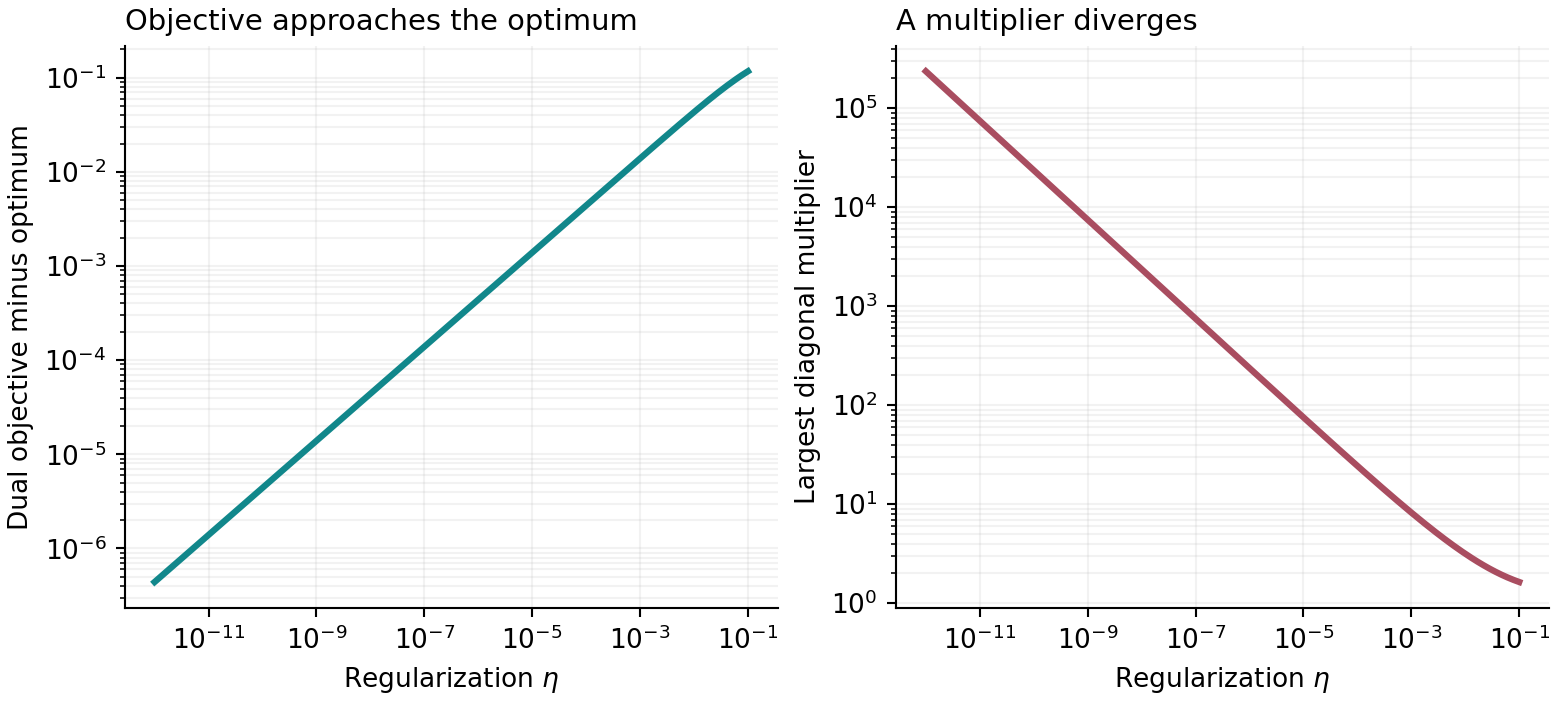
\includegraphics[width=\textwidth]{singular_dual_limit.png}
\caption{The explicit feasible dual sequence for $a=(0.3,0.2,0.5,0)$, $b=(0.3,0.2,0,0.5)$ and $p=(0.1,0.2,0.3,0.4)$. Its objective converges to the attained primal optimum while a multiplier diverges. Curves evaluate the exact formula; they are not solver output.}
\end{figure}

\section{Universality of higher-dimensional equality sets}\label{sec:universality}
The optimizer face is large enough to contain an arbitrary smaller bipartite fixed-marginal problem. This explains why a qubit-like unique normal form should not be expected in higher dimension.

\begin{theorem}[Embedding arbitrary residual quantum correlations]\label{thm:universality}
Let $\omega$ be any density matrix on $\C^r\otimes\C^s$ with specified marginals. There exist positive probability vectors $a,b$ in dimension $d=r+s$, with both lists decreasing, and an affine embedding of the whole fixed-marginal state space of $\omega$ into the optimizers of the marginal-spectrum FEF bound. Each embedded state has the form
\[
 \rho_\omega=zz^\dagger+\delta V\omega V^\dagger,\qquad \delta>0,
\]
and satisfies
\[
 f_d(\rho_\omega)=\frac1d\left(\sum_i\sqrt{m_i}\right)^2,
 \qquad \rank\rho_\omega=1+\rank\omega.
\]
The local product projection onto the residual subspaces extracts $V\omega V^\dagger$ with probability exactly $\delta$.
\end{theorem}
\begin{proof}
Diagonalize the two prescribed marginals of $\omega$, with eigenvalue vectors $a',b'$. Choose a strictly decreasing positive probability vector $\lambda$ of length $d$. Allocate disjoint index sets of sizes $r,s$ to the two residual spaces, and embed $a',b'$ on these respective sets as $\widetilde a,\widetilde b$. Choose $0<\delta<1$ sufficiently small that
\[
 \delta\max(\|\widetilde a\|_\infty,\|\widetilde b\|_\infty)
 <(1-\delta)\min_{i<d-1}(\lambda_i-\lambda_{i+1}).
\]
Set $m=(1-\delta)\lambda$, $a=m+\delta\widetilde a$ and $b=m+\delta\widetilde b$. They remain strictly decreasing positive probability vectors, and their componentwise minimum is $m$. The isometry $V$ embeds $\omega$ in the product of the disjoint residual spaces. The displayed state has marginals $\diag(a),\diag(b)$ and its Bell overlap is $(\sum\sqrt m)^2/d$. The universal spectral theorem proves that no other maximally entangled target does better. Orthogonality of the coherent and residual supports gives the rank identity and the local-projection statement. All choices depend only on the prescribed marginal pair, so the embedding is affine on the entire corresponding coupling space.
\end{proof}

\subsection{An exact four-dimensional family with different residual entanglement}
Take
\[
 m=\frac1{36}(16,9,4,1),\qquad
 a=\frac1{36}(19,9,7,1),\qquad
 b=\frac1{36}(16,12,4,4),\qquad\delta=\frac16.
\]
Here $I_+=\{0,2\}$, $I_-=\{1,3\}$, and
\[
 z=\frac16(4\ket{00}+3\ket{11}+2\ket{22}+\ket{33}).
\]
Let $\omega$ be any two-qubit state with both marginals $\Id_2/2$, embedded by $V\ket{i,j}=\ket{2i,2j+1}$. Then
\[
 \rho_\omega=zz^\dagger+\frac16V\omega V^\dagger,
 \qquad \boxed{f_4(\rho_\omega)=\frac{25}{36}.}
\]
For $\omega=\ket{\Phi^+}\bra{\Phi^+}$ the full state has rank two, and local projection onto even Alice and odd Bob levels yields a Bell pair with probability $1/6$. For $\omega=\Id_4/4$ the full state has rank five and the same projection yields a separable state. Both have exactly the same actual marginals and fully entangled fraction. The optimizer face has affine dimension nine. The coherent-plus-product sharpness witness is therefore only one point in a much larger equality set.

\section{Success probability versus conditional entangled fraction}\label{sec:success}
Local filtering is operational only after specifying its success probability. Here the input is a canonical two-qubit state $\sigma$ with $\sigma_B=\Id/2$ and centre length $c$. A single successful Bob Kraus operator $K$ satisfies $K^\dagger K\preceq\Id$; the successful state is normalized by its probability $q_K$.

\begin{theorem}[Sharp required-success frontier]\label{thm:success}
Let $0\le c\le1$ and $0<q\le1$. Over all such canonical inputs and filters with success probability at least $q$, the maximal conditional FEF is
\begin{equation}\label{eq:success-frontier}
 \boxed{
 G(c,q)=\begin{cases}
 1-c/2,&0<q\le1-c/2,\\[2mm]
 \displaystyle\frac{[1+\sqrt{(1-c)(2q-1)}]^2}{4q},&1-c/2\le q\le1.
 \end{cases}}
\end{equation}
Every value is attained. The two expressions agree at the transition. At $q=1$, the frontier is the canonical bound; allowing success $q=1-c/2$ reaches Milne's larger centre-only bound.
\end{theorem}
\begin{proof}
The input Bob marginal is uniform, so $q_K=\tr(K^\dagger K)/2$. If the normalized output Bob length is $b$, the two eigenvalues of $K^\dagger K$ are $q_K(1+b)$ and $q_K(1-b)$. Physical admissibility therefore implies
\[
 q_K(1+b)\le1,\qquad b\le\frac{1-q}{q}.
\]
For invertible filters the centre is unchanged and the joint frontier gives $f\le\Fe(c,b)$. Its unique peak is $b_*=c/(2-c)$ and it increases on $[0,b_*]$. Thus the optimal allowed value is $b=\min\{b_*,(1-q)/q\}$, which gives~\eqref{eq:success-frontier}. One elementary proof of monotonicity writes $x_b=\sqrt{1+b}$, $y_b=\sqrt{1-b}$ and $s=\sqrt{1-c}$. For $b\le B\le b_*$ one has $y_B\ge s x_B$ and
\[
 (x_B-x_b)(x_B+x_b)=(y_b-y_B)(y_b+y_B).
\]
Since $y_b+y_B\ge s(x_B+x_b)$, this implies $x_b+s y_b\le x_B+s y_B$.

For attainment take the canonical amplitude-damping state $\sigma_c$ of the equality classification and
\[
 K=\diag\bigl(\sqrt{q(1+b)},\sqrt{q(1-b)}\bigr)
\]
with the optimal $b$ just identified. It is a valid contraction, succeeds with probability exactly $q$, and gives $\rho_{c,b}$. A singular filter has success probability at most $1/2$, since its sole nonzero squared singular value is at most one. It is therefore infeasible when $q>1/2$; when $q\le1/2$, its product output has FEF at most $1/2\le1-c/2=G(c,q)$. Singular filters are needed for attainment only at the endpoint $c=1$, $q\le1/2$, where the successful state is a pure product. No singular whitening identity is used.
\end{proof}

\begin{figure}[htbp]\centering
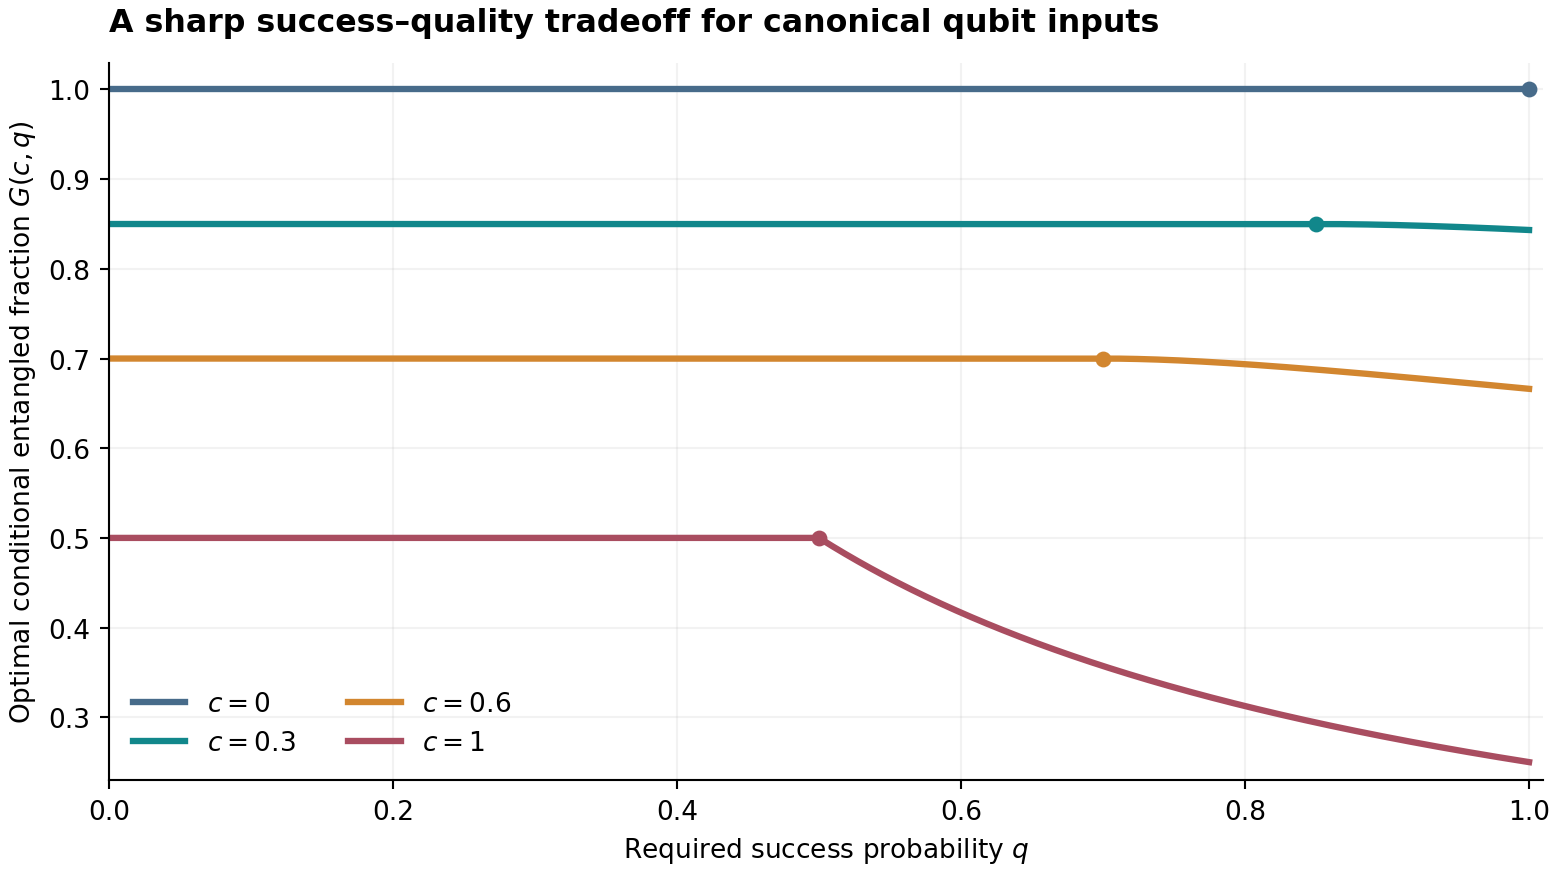
\includegraphics[width=.95\textwidth]{filter_success_frontier.png}
\caption{Exact required-success frontier. A marker identifies $q=1-c/2$, the largest required success at which Milne's centre-only value can still be attained. The curves apply to optimization over canonical inputs with the stated centre and physically allowed Bob filters.}
\end{figure}

\section{Quantitative rigidity of the extracted Schmidt spectrum}\label{sec:cap-stability}
Let $\alpha,\beta,p$ be as in the prescribed-Schmidt theorem, with $p_i>0$, $m_i=\min(\alpha_i,\beta_i)$ and $S=\sum_i\sqrt{p_i m_i}>0$. Let $t=\bra x\tau\ket x>0$ and $w=\tau x/\sqrt t$, and write $q_i$ for the decreasing squared Schmidt coefficients of $w$. The original proof gives $q_i\le m_i$ and
\[
 \sqrt t\le\sum_i\sqrt{p_i q_i}\le S.
\]
\begin{theorem}[Individual cap-deficit control]\label{thm:cap-stability}
For $\epsilon=S^2-t$,
\[
 \boxed{\sqrt{p_i}\,S\,(m_i-q_i)\le2\sqrt{m_i}\,\epsilon\quad\text{for every }i.}
\]
Consequently, writing $p_{\min}=\min_i p_i$ and $m_{\max}=\max_i m_i$,
\[
 \sum_i(m_i-q_i)
 \le\frac{2\sqrt{m_{\max}}}{S\sqrt{p_{\min}}}\,\epsilon.
\]
The residual positive matrix $\tau-ww^\dagger$ therefore has trace at most $1-\sum_i m_i$ plus this explicit error. At equality every cap is saturated.
\end{theorem}
\begin{proof}
Each nonnegative term satisfies
\[
 \sqrt{p_i}(\sqrt{m_i}-\sqrt{q_i})
 \le S-\sum_j\sqrt{p_jq_j}\le S-\sqrt t.
\]
Multiply by $\sqrt{m_i}+\sqrt{q_i}\le2\sqrt{m_i}$, then by $S$, and use
\[
 S(S-\sqrt t)\le S^2-t=\epsilon.
\]
This proves the individual bound, including $m_i=0$. For the aggregate estimate, first sum the square-root deficits with their weights, rather than summing the individual upper bounds:
\[
 \sqrt{p_{\min}}\sum_i(\sqrt{m_i}-\sqrt{q_i})
 \le S-\sum_i\sqrt{p_iq_i}\le\epsilon/S.
\]
Use $m_i-q_i\le2\sqrt{m_{\max}}(\sqrt{m_i}-\sqrt{q_i})$. This avoids an extraneous factor of $d$. This is spectrum rigidity of the canonical extraction, not a claim of universal trace-distance rigidity to a unique state; the high-dimensional optimizer faces above rule out such a uniqueness claim.
\end{proof}

\section{Complete higher-dimensional saturation geometry}\label{sec:spectral-saturation}

For a state $\rho$ on $\mathbb C^d\otimes\mathbb C^d$, write
\[
 f_d(\rho)=\max_{|e\rangle\ \text{maximally entangled}}
                  \langle e|\rho|e\rangle.
\]
Let $\alpha_1\ge\cdots\ge\alpha_d\ge0$ and
$\beta_1\ge\cdots\ge\beta_d\ge0$ be its marginal eigenvalues. Put
\[
 m_i=\min(\alpha_i,\beta_i),\qquad
 L=\sum_i m_i,\qquad \delta=1-L,
\]
\[
 I_A=\{i:\alpha_i>\beta_i\},\qquad
 I_B=\{i:\beta_i>\alpha_i\},\qquad
 |z_m\rangle=\sum_i\sqrt{m_i}|ii\rangle.
\]
The sets $I_A,I_B$ are disjoint. The sharp marginal-spectrum bound is
\begin{equation}\label{eq:marginal-fef}
 f_d(\rho)\le {1\over d}\left(\sum_i\sqrt{m_i}\right)^2.
\end{equation}

\subsection{All equality cases, including repeated and zero eigenvalues}

\paragraph{Theorem (complete saturation normal form).}
Equality in \eqref{eq:marginal-fef} holds if and only if, up to local unitaries,
\begin{equation}\label{eq:all-saturators}
 \rho=|z_m\rangle\langle z_m|+R,\qquad
 R\succeq0,\qquad
 \operatorname{supp}R\subseteq
       \operatorname{span}\{|ij\rangle:i\in I_A,\ j\in I_B\},
\end{equation}
where $\rho_A,\rho_B$ have the specified spectra $\alpha,\beta$.
There is no simplicity or full-rank assumption on either spectrum.

The remaining spectral condition has a smaller, explicit form. Write
$M_A=\operatorname{diag}(m_i:i\in I_A)$ and
$M_B=\operatorname{diag}(m_i:i\in I_B)$. Regarding $R$ as an operator on
$\mathbb C^{I_A}\otimes\mathbb C^{I_B}$, the permitted residuals are exactly
\[
 R\succeq0,\quad
 \operatorname{spec}(M_A+\operatorname{Tr}_B R)
                  =\{\alpha_i:i\in I_A\},\quad
 \operatorname{spec}(M_B+\operatorname{Tr}_A R)
                  =\{\beta_i:i\in I_B\}.
\]
In particular $\operatorname{Tr}R=\delta$. Either index set can be empty
only when $\alpha=\beta$; in that case $R=0$ and the saturator is pure.
The displayed characterization is of states with fixed marginal spectra.
For fixed marginal matrices one additionally imposes their matrix equalities.

\paragraph{Idea of the proof.} A saturating state contains the coherent
vector $z_m$ with the largest weights the marginals allow. Whatever is left
over is a positive residual whose marginals only add to the parts of the
spectra where one marginal exceeds the other. The lemma below handles
repeated eigenvalues, and positivity then confines the residual to the
rectangle $I_A\times I_B$, which the maximally entangled target does not
see.

\paragraph{A positive-perturbation lemma.}
Let $M=\operatorname{diag}(m_1,\ldots,m_d)$ with decreasing $m_i$, and
$Y\succeq0$. Suppose $M+Y$ has decreasing eigenvalues $a_i$.
For a maximal constant block $m_{k+1}=\cdots=m_{k+r}=\lambda$, let
$E_\lambda$ be its eigenspace and let
\[
 s=\#\{i\in\{k+1,\ldots,k+r\}:a_i>\lambda\}.
\]
Then $\dim(E_\lambda\cap\ker Y)\ge r-s$.

\emph{Proof.} The case $s=r$ is immediate. Otherwise monotonicity gives
$a_i\ge m_i$, so $M+Y$ has exactly $k+s$ eigenvalues strictly greater than
$\lambda$. On $V=E_{>\lambda}\oplus E_\lambda$, the compression of
$M+Y-\lambda I$ is positive semidefinite. Its kernel is exactly
$E_\lambda\cap\ker Y$: both nonnegative quadratic-form summands must
vanish, and a zero quadratic form of a positive operator is in its kernel.
Consequently this compression has a strictly positive subspace of dimension
$k+r-\dim(E_\lambda\cap\ker Y)$. The min--max principle bounds that
dimension by the number $k+s$ of positive eigenvalues of $M+Y-\lambda I$.
This proves the lemma. This argument also covers $\lambda=0$.

\paragraph{Proof of the theorem.}
Take a maximizing maximally entangled vector, and use local unitaries so it
is $|\Phi_d\rangle=d^{-1/2}\sum_i|ii\rangle$. Put
$t=\langle\Phi_d|\rho|\Phi_d\rangle$ and
$|w\rangle=\rho|\Phi_d\rangle/\sqrt t$. The zero case is irrelevant:
$L>0$ for probability spectra, so the upper bound being saturated is positive.
Positive-matrix Cauchy--Schwarz gives
\[
 R:=\rho-|w\rangle\langle w|\succeq0,\qquad
 \langle\Phi_d|w\rangle=\sqrt t.
\]
If $W$ is the coefficient matrix of $w$ and $q_i$ are its squared singular
values in decreasing order, partial trace and eigenvalue monotonicity give
$q_i\le m_i$. Therefore
\[
 \sqrt{dt}=\operatorname{Re}\operatorname{Tr}W
 \le\operatorname{Tr}\sqrt{W^\dagger W}
 =\sum_i\sqrt{q_i}\le\sum_i\sqrt{m_i}.
\]
Equality forces $q_i=m_i$ for every $i$ and $W\succeq0$.
For the latter assertion, write $W=UH$ in polar form: equality in
$\operatorname{Re}\operatorname{Tr}UH\le\operatorname{Tr}H$ forces
$U$ to be the identity on the range of $H$. A transformation
$U_0\otimes\overline{U_0}$ preserves $\Phi_d$ and diagonalizes $W$.
Thus $w=z_m$, and
\[
 \rho_A=M+R_A,\qquad \rho_B^T=M+R_B^T,
\]
with both residual marginals positive.

Consider any maximal constant block of $m$. The indices in that block with
$\alpha_i>m_i$ form a prefix, as do those with $\beta_i>m_i$. These two
prefixes cannot both be nonempty, since that would contradict
$m_i=\min(\alpha_i,\beta_i)$ at the first position of the block. Hence
at most one residual marginal is active on any such block. Apply the lemma
to both residual marginals. The inactive marginal annihilates the entire
block. The active marginal has at least as many kernel vectors in that
block as there are positions without surplus. Choose an orthonormal basis
of the block whose last vectors lie in that kernel. This basis choice
preserves both $M$ and $\Phi_d$, so it can be made independently on every
constant block. In the resulting bases
\[
 \operatorname{supp}R_A\subseteq\mathbb C^{I_A},\qquad
 \operatorname{supp}R_B\subseteq\mathbb C^{I_B}.
\]
Positivity upgrades marginal support to joint support. Indeed, for any local
kernel vector $u$, the nonnegative sum
$\sum_j\langle u,j|R|u,j\rangle=\langle u|R_A|u\rangle=0$
forces every $|u,j\rangle$ into $\ker R$. Applying this on both sides
gives the rectangle in \eqref{eq:all-saturators}.

Conversely, a positive residual on that rectangle is orthogonal to every
$|ii\rangle$, because $I_A\cap I_B=\varnothing$. Therefore
\[
 \langle\Phi_d|\rho|\Phi_d\rangle
       ={1\over d}\left(\sum_i\sqrt{m_i}\right)^2,
\]
and the spectral upper bound makes this the fully entangled fraction.
The smaller spectral conditions follow by splitting each marginal into
its active residual block and the unaffected diagonal complement.

\subsection{The same equality set for every full-Schmidt-rank target orbit}

Let $p_1\ge\cdots\ge p_d\ge0$ be a probability vector and define
\[
 F_p(\rho)=\max_{\substack{|x\rangle:\ \text{squared Schmidt coefficients }p}}
                  \langle x|\rho|x\rangle.
\]
The sharp overlap bound is
\[
 F_p(\rho)\le\left(\sum_i\sqrt{p_i m_i}\right)^2.
\]
For fixed marginal spectra $\alpha,\beta$, the following are equivalent:
\begin{enumerate}
\item $\lambda_{\max}(\rho)=L=\sum_i m_i$;
\item $\rho$ has the complete normal form \eqref{eq:all-saturators};
\item $f_d(\rho)=d^{-1}(\sum_i\sqrt{m_i})^2$;
\item for at least one decreasing probability vector $p$ with all $p_i>0$,
      $F_p(\rho)=(\sum_i\sqrt{p_i m_i})^2$;
\item for every decreasing probability vector $p$, including those with zero entries,
      $F_p(\rho)=(\sum_i\sqrt{p_i m_i})^2$.
\end{enumerate}
Thus the complete maximizing set is independent of every strictly positive
target Schmidt profile. This identifies all maximizers of the previously
known maximal-eigenvalue bound, not merely one family attaining its value.

\emph{Proof.} Suppose first that $\lambda_{\max}(\rho)=L$ and choose a
normalized top eigenvector $v$. The vector $w=\sqrt L\,v$ satisfies
$\rho\succeq|w\rangle\langle w|$. If $q_i$ are its decreasing squared
Schmidt coefficients, marginal positivity gives $q_i\le m_i$. But
$\sum_i q_i=L=\sum_i m_i$, so every inequality is an equality. Apply
independent local unitaries to put $w=z_m$ and use the positive-perturbation
lemma above. Its block argument depends only on the marginal spectra and
$q=m$, and therefore gives \eqref{eq:all-saturators}. Conversely, a state
in that normal form has $\rho z_m=Lz_m$, since the residual rectangle is
orthogonal to $z_m$. The general bound $\lambda_{\max}(\rho)\le L$
then makes its largest eigenvalue exactly $L$.

For the target-orbit assertion, choose a maximizing target $x$ and extract
$w=\rho x/\sqrt{\langle x|\rho|x\rangle}$ as before. The singular-value
trace inequality gives
\[
 \sqrt{\langle x|\rho|x\rangle}
 \le\sum_i\sqrt{p_i q_i}\le\sum_i\sqrt{p_i m_i}.
\]
If all $p_i>0$, equality forces every $q_i=m_i$. The same block argument
again gives the normal form. Conversely, in the normal-form bases the
target $x_p=\sum_i\sqrt{p_i}|ii\rangle$ is orthogonal to $R$ and has
overlap $(\sum_i\sqrt{p_i m_i})^2$. This works also when some $p_i=0$.
The maximally entangled target is the special case $p_i=1/d$, completing
all implications.

The condition that the one target profile in item 4 have no zero entry is
needed only on the positive cap support: the same equivalence holds whenever
$p_i>0$ for every $i$ with $m_i>0$. Indeed $q_i\le m_i=0$ already fixes
all remaining extracted Schmidt coefficients. For decreasing profiles this
condition says that the target Schmidt rank is at least
$r=\min(\operatorname{rank}\rho_A,\operatorname{rank}\rho_B)$.
Some positivity condition on the active support is necessary. For $d=2$, the state
\[
 \rho={1\over2}|00\rangle\langle00|
       +{1\over2}|11\rangle\langle11|
\]
has marginal spectra $\alpha=\beta=(1/2,1/2)$ and attains the product-target
cap $F_{(1,0)}=1/2$. Nevertheless its fully entangled fraction and largest
eigenvalue are both $1/2$, strictly below the corresponding caps $1$.

\paragraph{Prior-art boundary for the equivalence.}
Klyachko~\cite{klyachko}, Theorem 6.3.1, already proved that the
maximum possible largest eigenvalue for prescribed marginal spectra is
$\sum_i\min(\alpha_i,\beta_i)$. Immediately after that theorem he raised
the problem of describing its maximizers and discussed a representation-theoretic
recurrence for the associated spectra. The complete positive-residual
normal form and its equivalence with every full-Schmidt-rank overlap
maximization are the additional results proved here. A bounded search for
subsequent equality classifications found no matching statement; that search
does not establish worldwide priority or certify that the classification
problem remained open until this work.

\subsection{Exact rank-one coupling capacity in every dimension}

For positive integers $n\le m$, define the uniform-marginal coupling capacity
of a normalized pure target $x\in\mathbb C^n\otimes\mathbb C^m$ by
\[
 \mathsf a_{n,m}(x)=\max_{\substack{\rho\succeq0\\
                     \rho_A=I_n/n,\ \rho_B=I_m/m}}
                   \langle x|\rho|x\rangle.
\]
If $s_1,\ldots,s_n\ge0$ are the Schmidt amplitudes of $x$, then
\begin{equation}\label{eq:uniform-capacity}
 \boxed{\mathsf a_{n,m}(x)={1\over m}\left(\sum_{i=1}^n s_i\right)^2.}
\end{equation}
Equivalently, for arbitrary local dimensions the denominator is
$\max(n,m)$ and the sum runs over the $\min(n,m)$ Schmidt amplitudes.
For $n=m=d$ and every $s_i>0$, the optimizing coupling is unique:
it is the maximally entangled pure state in the target's Schmidt bases.

\emph{Elementary proof.} Use local unitaries to write
$x=\sum_{i=1}^n s_i|ii\rangle$. Put $d_i=\rho_{ii,ii}$.
The Bob marginal gives $0\le d_i\le1/m$, while positivity gives
$\operatorname{Re}\rho_{ii,jj}\le\sqrt{d_i d_j}\le1/m$.
Consequently
\[
 \langle x|\rho|x\rangle
   \le\left(\sum_i s_i\sqrt{d_i}\right)^2
   \le {1\over m}\left(\sum_i s_i\right)^2.
\]
This proof also permits zero Schmidt amplitudes. For sharpness, let
\[
 z={1\over\sqrt m}\sum_{i=1}^n|ii\rangle,\qquad
 \rho_*=|z\rangle\langle z|+
        {1\over nm}\sum_{i=1}^n\sum_{j=n+1}^m|ij\rangle\langle ij|.
\]
The sum is empty if $n=m$. Its Alice marginal is
$I_n/m+(m-n)I_n/(nm)=I_n/n$; its Bob marginal is $I_m/m$.
It is positive and its target overlap is the right side of
\eqref{eq:uniform-capacity}. In the square case with every $s_i>0$,
equality forces every $d_i=1/d$. These $d$ populations already sum to one,
so all other populations, and hence their rows and columns by positivity,
vanish. Equality in the off-diagonal estimates forces the remaining block
to have every entry $1/d$, giving the unique pure Bell coupling.

More generally, if every $s_i>0$ and $n<m$, the entire rectangular
optimizer face is
\[
 \rho=|z\rangle\langle z|+R,\quad R\succeq0,\quad
 \operatorname{supp}R\subseteq\mathbb C^n\otimes
                    \operatorname{span}\{|n+1\rangle,\ldots,|m\rangle\},
\]
\[
 R_A=(1/n-1/m)I_n,\qquad R_B=P_{\mathrm{tail}}/m.
\]
Indeed equality forces $\rho_{ii,ii}=1/m$ for all $i\le n$ and the
correlated principal block $zz^*$. The fixed Bob marginal forces every
other population in the first $n$ Bob columns to vanish. Positivity leaves
only a possible coherent cross vector $v$ between $z$ and the tail, but
the Bob off-diagonal entries between the first $n$ columns and the tail
are $m^{-1/2}v_{ij}$ or their conjugates; the prescribed diagonal Bob
marginal therefore forces $v=0$. The remaining partial traces are exactly
the displayed ones. Conversely every such residual attains the bound.
The face has affine dimension
\[
 (n^2-1)((m-n)^2-1).
\]
For $n<m$ the optimizer is unique precisely when $n=1$ or $m=n+1$;
for $n=m$ it is the unique pure Bell state. The two-by-three attainer below
is consequently unique for its displayed target.

\paragraph{Published capacity comparison.}
Proposition 3.5 of Skalski et al.~\cite{capacity2025} proves the lower bound
corresponding to \eqref{eq:uniform-capacity} in the square case and proves
equality when $d=2$. The formula above establishes equality for every $d$.
The paper does not label this particular all-dimensional extension as an
open problem. Its capacity $\alpha(E_x)$ equals $\mathsf a_{n,m}(x)$:
the paper's normalized-trace density $A_\sigma$ corresponds to the ordinary
trace-one matrix $\rho=A_\sigma/(nm)$, and the normalized-trace marginal
functionals correspond exactly to $I_n/n,I_m/m$.

The same paper's printed Theorem 3.7(ii), stated for $n\le m$, says that a
maximally entangled target has capacity one. With the paper's definition
of rectangular maximal entanglement, its Schmidt amplitudes are all
$1/\sqrt n$. Formula \eqref{eq:uniform-capacity} gives the corrected value
$n/m$, so the printed statement requires either $n=m$ or replacement of
one by $n/m$. In fact Cauchy--Schwarz in \eqref{eq:uniform-capacity}
proves the exact rectangular characterization
\[
 x\text{ is maximally entangled in }\mathbb C^n\otimes\mathbb C^m
 \quad\Longleftrightarrow\quad \mathsf a_{n,m}(x)=n/m.
\]

For a concrete counterexample to the printed rectangular value, take
\[
 x={|00\rangle+|11\rangle\over\sqrt2}\in\mathbb C^2\otimes\mathbb C^3,
 \qquad
 \rho_*={2\over3}|x\rangle\langle x|
       +{1\over6}\bigl(|02\rangle\langle02|+|12\rangle\langle12|\bigr).
\]
Both marginals are uniform, and the elementary bound above proves
$\mathsf a_{2,3}(x)=2/3<1$ exactly. The printed statement has this form in arXiv:2211.02401v3; no erratum was found in a bounded search. This is a correction of the displayed rectangular
statement; it does not affect the paper's square-dimensional statement
or its general duality theorem.

For completeness, the same paper's projective coupling capacity has the
particularly simple exact expression
\[
 \gamma(E_x)={r\over m},\qquad r=\operatorname{Schmidt\ rank}(x),\quad n\le m.
\]
Its defining feasibility condition is
$(P^\perp\otimes Q^\perp)x=0$ for local orthogonal projections $P,Q$.
If $X$ is the coefficient matrix of $x$, this condition writes $X$ as a
sum of a matrix with range in $\operatorname{ran}P$ and one whose right
support has dimension $\operatorname{rank}Q$. Thus
$r\le\operatorname{rank}P+\operatorname{rank}Q$, and the normalized cost
satisfies
\[
 {\operatorname{rank}P\over n}+{\operatorname{rank}Q\over m}
 \ge {r\over m}.
\]
Taking $P=0$ and $Q$ equal to the Bob Schmidt-support projection attains
this value. Hence $\alpha(E_x)=\gamma(E_x)$ exactly when all nonzero
Schmidt amplitudes are equal, by Cauchy--Schwarz.

The paper ends by asking whether its Proposition 3.10 extends beyond
dimension two. Part (i), which would say that a subspace supporting a
uniform-marginal coupling must contain a maximally entangled vector, has
a negative answer already in dimension three. Let $F$ be the swap and
$P_-=(I-F)/2$ the projection onto the antisymmetric subspace. The state
\[
 \rho_-={P_-\over3}={I-F\over6}
\]
has both marginals $I_3/3$ and is supported on $P_-$, so
$\alpha(P_-)=1$. Every vector in that subspace has a skew-symmetric
$3\times3$ coefficient matrix, whose determinant is zero since
$\det C=\det(-C^T)=-\det C$. It therefore has Schmidt rank at most two
and cannot be maximally entangled in dimension three. This uses the
standard antisymmetric state as an exact counterexample to the proposed
extension; it is not a new construction of that state. The formula for
$\gamma$ likewise gives the precise higher-dimensional replacement for
the rank-one part (ii). These observations are immediate consequences of
the displayed definitions and do not require a further conjectural step.

\subsection{The aligned face and sharp rank restriction}
For decreasing diagonal marginal matrices and a fixed target with positive
diagonal Schmidt amplitudes, the complete face is the coherent core plus
all residual couplings with marginals $\operatorname{diag}(\alpha-m)$ and
$\operatorname{diag}(\beta-m)$. This is the ordered specialization of
Theorems~\ref{thm:optimizer-face} and~\ref{thm:boundary-face}. Even when
some $m_i=0$, at most one marginal has a surplus in the final zero block,
so the possible zero-block cross rectangle in the general unordered
boundary theorem is empty.

For every spectral saturator the normal form gives
\[
 \operatorname{rank}\rho=1+\operatorname{rank}R
 \le1+|I_A||I_B|\le1+\lfloor d^2/4\rfloor.
\]
This is sharp for every $d\ge2$: choose a positive strictly decreasing
$m$ of sum $1-\delta$, partition the surplus indices as evenly as possible,
and distribute the two residual masses positively on opposite sides.
For sufficiently small $\delta$, both marginal lists remain decreasing.
The product residual is positive definite on its rectangle and attains
the bound. This is consistent with the more general fixed-target theorem
in Section~\ref{sec:all-optimizer-rank}; it describes every saturator,
whereas Theorem~\ref{thm:low-rank-pure-target} guarantees a smaller-rank
attaining representative.

\subsection{Every saturator has the largest possible Schmidt number}

\paragraph{Theorem.}
Every state saturating \eqref{eq:marginal-fef} has
\[
 \operatorname{SN}(\rho)
       =\min\{\operatorname{rank}\rho_A,\operatorname{rank}\rho_B\}.
\]
This conclusion includes all degeneracies and rank-deficient marginal states.

\emph{Proof.} Let $r=\#\{i:m_i>0\}$, which equals the displayed minimum
of local ranks. In the normal form, the support of $\rho$ is the orthogonal
sum of $\operatorname{span}\{z_m\}$ and $\operatorname{supp}R$.
Every vector in that support has a coefficient matrix
\[
 C=a\operatorname{diag}(\sqrt{m_1},\ldots,\sqrt{m_d})+N,
 \qquad N_{ij}=0\quad\hbox{unless }i\in I_A, j\in I_B.
\]
Reorder the first $r$ indices by placing $I_A$ first and $I_B$ last.
The leading $r\times r$ block becomes upper triangular apart from its
diagonal, and therefore
\[
 \det C_{[r],[r]}=a^r\prod_{i=1}^r\sqrt{m_i}.
\]
For $a\ne0$ this minor is nonzero, so the vector has Schmidt rank at least
$r$. Every pure-state decomposition of $\rho$ contains a vector with
$a\ne0$, because its expectation on $z_m$ is nonzero. Hence its maximum
Schmidt rank is at least $r$, proving $\operatorname{SN}(\rho)\ge r$.
Every vector in the support of any bipartite state lies in the tensor product
of its marginal supports, giving the reverse bound $\operatorname{SN}(\rho)
\le\min(\operatorname{rank}\rho_A,\operatorname{rank}\rho_B)=r$.

\subsection{Fixed partial-transpose inertia and one-copy distillability}

Write $\Gamma$ for the partial transpose on Bob. If every $m_i>0$, every
saturator has the exact partial-transpose inertia
\[
 \boxed{\quad
 n_+(\rho^\Gamma)={d(d+1)\over2},\qquad
 n_-(\rho^\Gamma)={d(d-1)\over2},\qquad n_0(\rho^\Gamma)=0.
 \quad}
\]
The statement permits an arbitrary positive quantum residual in the normal
form. If exactly $r$ cap eigenvalues are positive, then
$n_-(\rho^\Gamma)\ge r(r-1)/2$. Whenever $r\ge2$, a single copy can be
locally projected with positive probability to an entangled two-qubit state;
thus every such saturator is one-copy distillable.

\emph{Proof.} Put $T=I_A\times I_B$ and let
$T'=\{(j,i):(i,j)\in T\}$. These coordinate sets are disjoint. In the
paired bases of $T$ and $T'$, the corresponding partial-transpose block is
\[
 H=\begin{pmatrix}C&D\\D&0\end{pmatrix},\qquad
 C=(R^\Gamma)_{T,T}=C^\dagger,\qquad
 D=\operatorname{diag}(\sqrt{m_i m_j}:(i,j)\in T)>0.
\]
There are no couplings from this block to its complement. The invertible
shear
\[
 S=\begin{pmatrix}I&0\\-\tfrac12D^{-1}C&I\end{pmatrix}
 \quad\hbox{satisfies}\quad
 S^\dagger H S=\begin{pmatrix}0&D\\D&0\end{pmatrix}.
\]
Sylvester's law of inertia therefore gives $|T|$ positive and $|T|$
negative eigenvalues on this block. Every remaining unordered pair
$\{i,j\}$ gives the unchanged two-dimensional block with eigenvalues
$\pm\sqrt{m_i m_j}$, and each diagonal vector $|ii\rangle$ gives the
positive eigenvalue $m_i$. Counting these blocks proves the full-rank
formula. Applying the same argument to the principal compression onto the
first $r$ indices on both sides, followed by eigenvalue interlacing, proves
the lower bound when some $m_i$ vanish.

Finally fix any $i\ne j$ with $m_i,m_j>0$ and project both local spaces
onto $\operatorname{span}\{|i\rangle,|j\rangle\}$. The coherent term
survives. The residual rectangle contributes at most one of the two
populations $|ij\rangle\langle ij|$ and $|ji\rangle\langle ji|$.
The projected state's partial transpose consequently has a principal
two-dimensional block of the form
\[
 \begin{pmatrix}\kappa&\sqrt{m_i m_j}\\
                 \sqrt{m_i m_j}&0\end{pmatrix}
 \quad\hbox{or its reversed ordering},\qquad \kappa\ge0,
\]
whose determinant is $-m_i m_j<0$. Its negative direction has Schmidt
rank two. The local projection succeeds with probability at least
$m_i+m_j>0$, proving the asserted one-copy distillability.

\subsection{An exact convex-roof entanglement value}

For full-rank $m$, use the standard normalization of the $G$-concurrence:
for a normalized pure state with coefficient matrix $C$,
$G_d(C)=d|\det C|^{2/d}$. Let $G_d(\rho)$ be its convex roof and
$G_d^{\mathrm a}(\rho)$ the concave roof over pure-state decompositions.
Then every saturator has the exact values
\[
 G_d(\rho)=G_d^{\mathrm a}(\rho)
                   =d\left(\prod_{i=1}^d m_i\right)^{1/d}.
\]
In fact every pure-state decomposition has the same average $G$-concurrence.
For any normalized support vector $C=a\operatorname{diag}\sqrt m+N$,
the triangular determinant identity gives
$G_d(C)=d|a|^2(\prod_i m_i)^{1/d}$. For a decomposition of $\rho$,
the expectation of the projection onto $z_m/\sqrt L$ gives
$\sum_k p_k|a_k|^2=1$. Averaging proves the formula without optimization.

This affine-roof mechanism has prior art: Gour and Guo~\cite{gourguo}, Theorem 7, characterize equality of $G$-concurrence and assistance using
nilpotent subspaces. The rectangle matrices here square to zero after
diagonal rescaling. The new connection established above is that every
marginal-spectrum FEF maximizer lies in this class, with the displayed
entanglement value fixed entirely by the two marginal spectra.

\subsection{Explicit quasidistillation, including quantum residuals}

Let $r=\#\{i:m_i>0\}$, put $\mu=\min_{i\le r}m_i$, and write a saturator in
the normal form. Let $D$ be diagonal with $D_i=m_i^{-1/4}$ for $i\le r$
and $D_i=0$ otherwise, and put
$\widetilde R=(D\otimes D)R(D\otimes D)$, with
$r_R=\operatorname{Tr}\widetilde R$. For $0<\varepsilon\le1$, define
diagonal filters
\[
 A_\varepsilon=\mu^{1/4}D\operatorname{diag}(\varepsilon^{a_i}),\qquad
 B_\varepsilon=\mu^{1/4}D\operatorname{diag}(\varepsilon^{1-a_i}),
\]
where $a_i=1$ on $I_A$, $a_i=0$ on $I_B$, and $a_i=1/2$ otherwise.
Both are contractions, since every retained diagonal factor
$\mu^{1/4}m_i^{-1/4}\varepsilon^{a_i}$ is at most one and the other
entries vanish. Direct multiplication
gives the unnormalized output and its success probability:
\[
 (A_\varepsilon\otimes B_\varepsilon)\rho
 (A_\varepsilon\otimes B_\varepsilon)^\dagger
 =\mu\varepsilon^2\bigl(r|\Phi_r\rangle\langle\Phi_r|
                               +\varepsilon^2\widetilde R\bigr),
\]
\[
 P_\varepsilon=\mu\varepsilon^2(r+\varepsilon^2r_R),\qquad
 F_\varepsilon:=\langle\Phi_r|\rho_\varepsilon|\Phi_r\rangle
                         ={r\over r+\varepsilon^2r_R}.
\]
Here $\Phi_r=r^{-1/2}\sum_{i=1}^r|ii\rangle$ is embedded in the original
space. Because $\widetilde R\perp\Phi_r$, the trace distance is exact:
\[
 {1\over2}\|\rho_\varepsilon-|\Phi_r\rangle\langle\Phi_r|\|_1
                =1-F_\varepsilon.
\]
For $\varepsilon^2\lambda_{\max}(\widetilde R)\le r$, the displayed Bell
vector is also a top eigenvector, and the fully entangled fraction within
the surviving $r\times r$ subspace equals $F_\varepsilon$.
Thus every saturator can approach the maximally entangled state of the
largest dimension permitted by its marginal ranks, even when its
residual $R$ is entangled and has off-diagonal coherences. For $R\ne0$ the
exact protocol relation, for sufficiently large $F$, is
\[
 P={\mu r^2\over r_R}{1-F\over F^2}\qquad(r_R>0).
\]
This is an attained protocol curve, not a claim of globally optimal success
probability. If $r_R=0$, the projected output is already exactly $\Phi_r$
with positive success probability $\mu r\varepsilon^2$; this can happen
for a mixed original state when $r<d$. When $r=d$, a mixed saturator
cannot yield an exact $d$-dimensional Bell
state in a single nonzero-probability local-filter branch: full Schmidt
rank of the output would require both local filters to be invertible,
whereas invertible filtering preserves the state's rank.

\subsection{Nonuniqueness even for fixed, simple marginal matrices}

Take $d=4$ and
\[
 \alpha=(2/5,3/10,1/5,1/10),\quad
 \beta=(7/20,33/100,17/100,3/20),\quad
 m=(7/20,3/10,17/100,1/10).
\]
All three lists have strictly decreasing positive entries. Here
$I_A=\{1,3\}$, $I_B=\{2,4\}$, $L=23/25$, and $\delta=2/25$.
Let
\[
 C={1\over20}|1\rangle\langle1|+{3\over100}|3\rangle\langle3|,
 \qquad
 D={3\over100}|2\rangle\langle2|+{1\over20}|4\rangle\langle4|.
\]
The product residual $R_0=C\otimes D/\delta$ and the pure residual
\[
 R_1=|r\rangle\langle r|,\qquad
 |r\rangle=\sqrt{1/20}|1,4\rangle+\sqrt{3/100}|3,2\rangle
\]
have exactly the same partial traces $C,D$. Consequently
\[
 \rho_s=|z_m\rangle\langle z_m|+(1-s)R_0+sR_1,\qquad0\le s\le1,
\]
all have the same fixed marginal matrices $\operatorname{diag}\alpha$ and
$\operatorname{diag}\beta$, and all attain the same sharp fully entangled
fraction. Nevertheless their purity varies:
\[
 \operatorname{Tr}\rho_s^2
 = {135713\over160000}+{3\over16000}s+{141\over32000}s^2.
\]
In particular $\rho_0$ and $\rho_1$ have purities $135713/160000$ and
$533/625$, and have ranks five and two respectively. They cannot be locally
unitarily equivalent. This gives an explicit continuum of inequivalent
saturators even with simple spectra and fixed marginal matrices. All of
them have Schmidt number four by the preceding theorem.

\subsection{Maximal Schmidt number with a small fully entangled fraction}

The Schmidt-number conclusion is stronger than certification by a large
fully entangled fraction alone. Consider the four-dimensional state
\[
 |z\rangle={1\over2}|00\rangle+
       {1\over10}(|11\rangle+|22\rangle+|33\rangle),\qquad
 \rho=|z\rangle\langle z|+{6\over25}\sum_{j=1}^3|0j\rangle\langle0j|.
\]
Its marginals are
\[
 \rho_A=\operatorname{diag}(97/100,1/100,1/100,1/100),\qquad
 \rho_B=I/4.
\]
It attains the spectral bound with
\[
 f_4(\rho)={4\over25}<{1\over4},\qquad
 \operatorname{SN}(\rho)=4,\qquad
 G_4(\rho)=G_4^{\mathrm a}(\rho)={\sqrt5\over25}.
\]
Thus even a saturator below the usual unfiltered teleportation threshold
can possess entanglement of the maximum available dimension. The explicit
filters above have $\mu=1/100$ and $r_R=72/5$, so
\[
 F_\varepsilon={5\over5+18\varepsilon^2},\qquad
 P_\varepsilon={\varepsilon^2(25+90\varepsilon^2)\over625}.
\]
The Bell overlap equals the output fully entangled fraction for
$\varepsilon^2\le5/6$, and tends to one as the success probability tends
to zero. The state has rank four, with eigenvalues
$7/25,6/25,6/25,6/25$ and twelve zeros.

\subsection{Prior-art and formal-verification scope}

Klyachko's 2004 maximal spectral-norm theorem gives $\lambda_{\max}\rho\le L$
with sharp value and a representation-theoretic discussion of maximizers;
that value is not a new result here.
Baio et al.~\cite{baio}, Theorem 2, establish quasidistillability for a
rank-one maximally correlated component plus a \emph{classical diagonal}
residual precisely when the residual's directed support is acyclic. That
older filtering mechanism covers the classical instances above. The theorem
here classifies every saturator of the weighted marginal FEF bound, permits
arbitrary quantum residuals on the forced rectangle, and yields the exact
Schmidt-number consequence. No claim of worldwide priority is certified by
the bounded literature search.

The saturation classification, its degeneracy argument, the Schmidt-number,
partial-transpose inertia, one-copy distillability and quasidistillation
consequences, the maximizing-face dimension, and the
$G$-concurrence calculation are exact analytic proofs. They are not
yet end-to-end Lean theorems. The \texttt{PopulationOverlap} section of \texttt{AllProofs.lean}
formalizes an end-to-end actual-complex-matrix optimization using target-basis
marginal populations, with a genuine positive trace-one attaining matrix.
That result needs no spectral or singular-value hypotheses.

\section{A robust certificate of maximal Schmidt number}\label{sec:robust-sn}
Assume $d\ge2$. The explicit dual in Theorem~\ref{thm:dual} only uses the diagonal
populations of the marginal matrices. Consequently its gap identity and
support bound remain valid if the actual marginal matrices have arbitrary
off-diagonal entries. Let these populations be $a_i,b_i$, assume
$m_i=\min(a_i,b_i)>0$, and let the normalized target be
$x=\sum_i s_i|ii\rangle$ with every $s_i>0$.
Set
\[
 S=\sum_i s_i\sqrt{m_i},\quad L=\sum_i m_i,\quad
 z=\sum_i\sqrt{m_i}|ii\rangle,\quad
 I_A=\{i:a_i>b_i\},\quad I_B=\{i:b_i>a_i\}.
\]
Let $P$ project onto
$K=\operatorname{span}\{z\}\oplus
\operatorname{span}\{|ij\rangle:i\in I_A,j\in I_B\}$,
and use $Q=\Id-P$ in this section. With
$\gamma_0=(S/2)\min_i(s_i/\sqrt{m_i})$, the dual slack $Z$ from
Theorem~\ref{thm:dual} satisfies
\begin{equation}\label{eq:dual-exact-deficit}
 \epsilon=S^2-\langle x|\rho|x\rangle=\tr(\rho Z),
 \qquad Z\succeq\gamma_0 Q.
\end{equation}
This gives a noise-tolerant certificate of the maximum Schmidt number,
not just a description of exact equality states.

Put $|\zeta\rangle=z/\sqrt L$ and
\[
 c_m={(d-1)^{d-1}\prod_i m_i\over L^d}.
\]
For \emph{every} density matrix $\omega$ of Schmidt number at most $d-1$,
whether or not it has the populations above,
\begin{equation}\label{eq:schmidt-support-witness}
 \operatorname{Tr}\omega Q\ge
       c_m\bigl(\langle\zeta|\omega|\zeta\rangle\bigr)^d.
\end{equation}
Here $K,P,Q$ use the displayed $z$ and disjoint rectangle $I_A\times I_B$.

\emph{Proof.} First let $\omega=|\psi\rangle\langle\psi|$ have Schmidt
rank at most $d-1$, and let $C$ be its coefficient matrix, with Frobenius
norm one. The projection $P\psi$ has coefficient matrix
\[
 C_K=a\operatorname{diag}\sqrt m+N,
 \qquad N_{ij}=0\ \text{outside }I_A\times I_B.
\]
Because the two index sets are disjoint, a simultaneous permutation puts
$N$ strictly above the diagonal. Thus
$|\det C_K|=|a|^d\sqrt{\prod_i m_i}$.
Let $\sigma_1\ge\cdots\ge\sigma_d$ be its singular values.
Since $C$ has a nonzero kernel vector,
\[
 \sigma_d\le\|C-C_K\|_{\mathrm{op}}\le\|C-C_K\|_{\mathrm F}
                         =\sqrt{\langle\psi|Q|\psi\rangle}.
\]
The other singular values satisfy
\[
 \prod_{j=1}^{d-1}\sigma_j
 \le\left({\sum_{j=1}^{d-1}\sigma_j^2\over d-1}\right)^{(d-1)/2}
 \le(d-1)^{-(d-1)/2},
\]
because $\|C_K\|_{\mathrm F}\le1$. Multiplying and squaring gives
\[
 \langle\psi|Q|\psi\rangle
       \ge(d-1)^{d-1}\left(\prod_i m_i\right)|a|^{2d}
       =c_m|\langle\zeta|\psi\rangle|^{2d}.
\]
For a mixed state of Schmidt number at most $d-1$, choose a decomposition
into such vectors and average. Jensen's inequality for $u\mapsto u^d$
gives \eqref{eq:schmidt-support-witness}.

Combining the witness with \eqref{eq:dual-exact-deficit}, a state with the
specified local populations is certified to have Schmidt number $d$ whenever
\[
 S^2-\langle x|\rho|x\rangle
 <\gamma_0c_m\bigl(\langle\zeta|\rho|\zeta\rangle\bigr)^d.
\]
This is a quantitative, directly testable sufficient criterion. No optimality
is claimed for its constant. At an exact spectral-FEF saturator,
$\langle\zeta|\rho|\zeta\rangle=L$ and the deficit is zero, so the
criterion recovers maximal Schmidt number and tolerates a nonzero error.


The assumptions $m_i>0$ and $s_i>0$ keep the displayed gap positive.
The associated projected-state estimate controls distance to the forced
support subspace, not to a state with exactly the same marginal matrices.
General Schmidt-number witnesses and $G$-concurrence lower bounds have
substantial prior literature~\cite{terhalhorodecki,sentis}; the displayed
witness is tailored here to the coherent-core/rectangle geometry.
It has an exact analytic proof and seeded falsification tests, and is
not included among the end-to-end Lean theorems.

\section{Negativity throughout a fully-entangled-fraction maximizing face}
\label{sec:negativity-face}

The saturation classification fixes the fully entangled fraction and the
$G$-concurrence, but it does not fix the negativity.  Here we solve the
minimum-negativity problem on every full-positive coherent-core rectangle,
and obtain both endpoints exactly on an infinite family of spectral
maximizer faces. We use the convention
$\mathcal N(\rho)=(\|\rho^\Gamma\|_1-1)/2$.
The conclusions concern the FEF-maximizing face under discussion; they do
not assert that its largest negativity is the largest among all states
with the same marginals.

Let $m_i>0$, $z=\sum_{i=1}^d\sqrt{m_i}\,|ii\rangle$, and let $I,J$ be
nonempty disjoint subsets of $\{1,\ldots,d\}$. Put
$L=\sum_i m_i$, $\delta=1-L>0$. Consider
\[
 \rho_R=|z\rangle\langle z|+R,
 \quad R\succeq0,\quad
 \operatorname{supp}R\subseteq\mathbb C^I\otimes\mathbb C^J,
 \quad \operatorname{Tr}_B R=\operatorname{diag}(u),\quad
 \operatorname{Tr}_A R=\operatorname{diag}(v),
\]
where $u_i,v_j>0$ and $\sum_i u_i=\sum_jv_j=\delta$.
This includes aligned fixed-matrix faces of full-rank spectral saturators,
as well as aligned fixed-population optimizer faces without any spectral
ordering assumption. No assertion is made that every prescribed-spectrum
optimizer admits this extra simultaneous alignment of its residual
marginals with the core. Without the spectral ordering condition, the
more general aligned face maximizes overlap with a fixed pure target;
FEF optimality over varying target bases is not asserted. Define
\[
 d_{ij}=\sqrt{m_i m_j},\qquad
 N_0=\sum_{1\le i<j\le d}\sqrt{m_i m_j}
                -\sum_{i\in I,j\in J}d_{ij}.
\]
The omitted pairs are distinct because $I\cap J=\varnothing$.

\subsection{A strict-convexity lemma for a saddle matrix}

\begin{lemma}\label{lem:strict-saddle}
For every positive definite $D\in M_n(\mathbb C)$, the function
\[
 C\longmapsto F_D(C)=
 \left\|\begin{pmatrix}C&D\\D&0\end{pmatrix}\right\|_1
\]
is strictly convex on the real vector space of Hermitian $n\times n$
matrices.
\end{lemma}
\begin{proof}
Write $H(C)$ for the displayed block matrix. It is invertible: the bottom
block of $H(C)(x,y)^T=0$ gives $Dx=0$, hence $x=0$ and then $Dy=0$.
For an invertible Hermitian matrix $H$, the maximizer of
$\operatorname{Tr}(SH)$ over Hermitian contractions $-I\preceq S\preceq I$
is unique and equals $\operatorname{sign}(H)$. This follows by diagonalizing
$H$: each diagonal entry of a maximizing contraction must have the sign
of the corresponding eigenvalue, and a contraction with a diagonal entry
of modulus one has zero off-diagonal entries in that row and column.

Suppose equality holds in convexity between $H(C_1)$ and $H(C_2)$ at an
interior mixing parameter. The unique supporting contraction of their
invertible mixture maximizes both endpoints, so
$S=\operatorname{sign}H(C_1)=\operatorname{sign}H(C_2)$.
Write $S=\begin{psmallmatrix}A&B\\B^*&E\end{psmallmatrix}$.
Since $H(C_1)S=|H(C_1)|\succ0$, its lower-right block $DB$ is positive
definite. Thus $B$ is invertible. Both $H(C_i)$ commute with $S$, hence
$\operatorname{diag}(C_1-C_2,0)$ commutes with $S$. Its upper-right
commutator block is $(C_1-C_2)B=0$. Invertibility of $B$ gives
$C_1=C_2$, proving strict convexity.
\end{proof}

Positive definiteness of $D$ matters. For
$D=\operatorname{diag}(1,0)$ and $C_t=\operatorname{diag}(0,t)$,
$F_D(C_t)=2+t$ for $t\ge0$; strict convexity fails.

\subsection{The unique minimum is a classical transportation problem}

\begin{theorem}\label{thm:negativity-transport}
The map $R\mapsto\mathcal N(\rho_R)$ is strictly convex. Its unique minimum
on the prescribed residual-marginal face is attained by a diagonal
residual
\[
 R_* = \sum_{i\in I,j\in J}t^*_{ij}|ij\rangle\langle ij|,
\]
where $t^*$ is the unique solution of the strictly convex transportation
problem
\[
 \boxed{\quad
 \min_{\substack{t_{ij}\ge0,\ \sum_jt_{ij}=u_i\\
                        \sum_it_{ij}=v_j}}
 \left[N_0+\frac12\sum_{i\in I,j\in J}
       \left(\sqrt{t_{ij}^2+4m_i m_j}-t_{ij}\right)\right].
 \quad}
\]
For every nondiagonal $R$, deleting its off-diagonal entries strictly
reduces $\mathcal N(\rho_R)$ and preserves both actual marginal matrices.
\end{theorem}
\begin{proof}
In the ordered bases of $I\times J$ and the reversed rectangle
$J\times I$, the varying partial-transpose block is
\[
 H(C)=\begin{pmatrix}C&D\\D&0\end{pmatrix},
 \quad C=R^\Gamma,\quad D=\operatorname{diag}(d_{ij})\succ0.
\]
All other diagonal and two-dimensional blocks are fixed. Consequently
\[
 \mathcal N(\rho_R)=N_0+\frac{F_D(R^\Gamma)-\delta}{2}.
\]
Partial transpose is an injective real-linear map on Hermitian matrices,
so Lemma~\ref{lem:strict-saddle} implies strict convexity.

Average the local unitaries $U\otimes\overline U$ over all diagonal
sign matrices $U$. They fix $z$, preserve the diagonal marginal matrices,
and delete precisely the off-diagonal entries of $R$. The characters
$\varepsilon_i\varepsilon_j$ on the disjoint rectangle are distinct.
Negativity is invariant under each local unitary and convex under their
mixture. Strict convexity makes the inequality strict unless every
conjugate is the same, which is equivalent to $R$ being diagonal.
For a diagonal residual the paired block eigenvalues are
$(t_{ij}\pm\sqrt{t_{ij}^2+4d_{ij}^2})/2$; summing their negative parts gives
the displayed objective. Each scalar cost has second derivative
$2d_{ij}^2/(t^2+4d_{ij}^2)^{3/2}>0$.
The compact nonempty transportation polytope therefore has exactly one
minimizer, which is also the unique quantum minimizer.
\end{proof}

This gives an exact efficient convex characterization even when the
minimizing transport is not a product coupling. Its optimality conditions
are particularly simple: there exist real potentials $\lambda_i,\mu_j$
such that, with
$g_{ij}'(t)=\tfrac12(t/\sqrt{t^2+4d_{ij}^2}-1)$,
\[
 \lambda_i+\mu_j=g'_{ij}(t^*_{ij})\quad(t^*_{ij}>0),
 \qquad \lambda_i+\mu_j\le-\tfrac12\quad(t^*_{ij}=0).
\]
These conditions are necessary and sufficient. For positive cells set
$h_{ij}=1+2\lambda_i+2\mu_j\in(0,1)$; then
$t^*_{ij}=2d_{ij}h_{ij}/\sqrt{1-h_{ij}^2}$.

\begin{corollary}[A closed sharp lower bound]\label{cor:negativity-total}
Put $P=(\sum_{i\in I}\sqrt{m_i})(\sum_{j\in J}\sqrt{m_j})$.
Then every residual satisfies
\[
 \boxed{\quad \mathcal N(\rho_R)\ge
 N_0+\frac{\sqrt{\delta^2+4P^2}-\delta}{2}.\quad}
\]
Equality holds exactly when
\[
 R=\sum_{i,j}\frac{\delta\sqrt{m_i m_j}}{P}
                         |ij\rangle\langle ij|.
\]
In particular, equality is feasible exactly when
$u_i=\delta\sqrt{m_i}/\sum_{k\in I}\sqrt{m_k}$ and
$v_j=\delta\sqrt{m_j}/\sum_{\ell\in J}\sqrt{m_\ell}$.
\end{corollary}
\begin{proof}
First dephase as in the theorem. The triangle inequality in $\mathbb R^2$
gives
$\sum_{i,j}\sqrt{t_{ij}^2+4d_{ij}^2}\ge
\sqrt{(\sum t_{ij})^2+4(\sum d_{ij})^2}$.
All $d_{ij}>0$, so equality holds exactly when $t_{ij}/d_{ij}$ is constant.
Trace $\delta$ fixes that constant to $\delta/P$. Strictness under
dephasing gives the full quantum equality statement.
\end{proof}

\paragraph{An exact nonproduct minimizer.}
The usual product residual need not minimize negativity, even within a
spectral FEF-maximizer face. Put
\[
 k=\frac{17}{3}+\frac4{\sqrt{21}},\quad
 a=\left(\frac{101}{50}+\frac{k}{10}\right)^{-1},\quad
 b=\frac a{100},\quad d_0=\frac a{10},\quad \delta=kd_0.
\]
Take $m=(a,a,b,b)$, $I=\{1,2\}$, $J=\{3,4\}$, and let
\[
 t^*=d_0\begin{pmatrix}4/\sqrt{21}&3/2\\3/2&8/3\end{pmatrix},
 \qquad u=v=t^*\binom11.
\]
Normalization follows from $2a+2b+\delta=1$. Both prescribed marginals
can be put in decreasing order by permutations within the two equal-core
blocks. Indeed $b+\max_jv_j=(1/100+5/12)a<a$.
The KKT potentials $\lambda=(-1/5,-1/10)$ and $\mu=(-1/10,0)$ have
sums $(-3/10,-1/5;-1/5,-1/10)$, exactly the four cost derivatives at
$t^*$. Thus the unique minimum is
\[
 \mathcal N_{\min}=a+b+d_0\left(\frac43+\frac3{\sqrt{21}}\right).
\]
But
$\det(t^*/d_0)=32/(3\sqrt{21})-9/4>0$, since
$128^2>27^2\cdot21$. The product transport $uv^T/\delta$ has determinant
zero and is different. Strict convexity therefore makes its negativity
strictly larger. This example distinguishes the coherent-minimum product
construction, which proves sharpness of the FEF bound, from the residual
that minimizes a different entanglement measure on the same optimal face.

\subsection{A quantitative penalty for residual coherence}

There is also an explicit, nonoptimal stability estimate. Let
$d_- =\min_{i,j}d_{ij}>0$, $d_+=\max_{i,j}d_{ij}$ and
\[
 h=\frac{\sqrt{\delta^2+4d_-^2}-\delta}{2},\qquad
 \kappa=\frac{h^2}{8d_+^2(\delta+d_+)}.
\]
For the diagonal dephasing $\Delta R$,
\begin{equation}\label{eq:negativity-coherence-gap}
 \mathcal N(\rho_R)-\mathcal N(\rho_{\Delta R})
       \ge \kappa\,\|R-\Delta R\|_2^2,
\end{equation}
where $\|\cdot\|_2$ is the Hilbert--Schmidt norm.
To prove this, along every residual segment we have
$\|C\|\le\|C\|_2=\|R\|_2\le\delta$ and
$\|H(C)\|\le M=\delta+d_+$.
For an eigenpair $H(C)(x,y)=\lambda(x,y)$, $x\ne0$ and
\[
 \lambda^2\|x\|^2-\lambda\langle x,Cx\rangle-\|Dx\|^2=0.
\]
It follows that $|\lambda|^2+\delta|\lambda|\ge d_-^2$, hence
$|H(C)|\succeq hI$. If
$S=\operatorname{sign}H=\begin{psmallmatrix}A&B\\B^*&E\end{psmallmatrix}$,
then $DB=(|H|)_{22}\succeq hI$, so
$\sigma_{\min}(B)\ge h/d_+$.
For a Hermitian perturbation $Q$ in the upper-left block, the spectral
second-derivative formula gives
\[
 F_D''(C)[Q,Q]
 =4\sum_{\lambda_r>0>\lambda_s}
      \frac{|\langle r,\operatorname{diag}(Q,0)s\rangle|^2}
           {\lambda_r-\lambda_s}
 \ge\frac{\|[\operatorname{diag}(Q,0),S]\|_2^2}{4M}
 \ge\frac{h^2}{2Md_+^2}\|Q\|_2^2.
\]
The same formula is valid with repeated eigenvalues, because the positive
and negative spectral subspaces stay separated from zero; repeated values
within one sign contribute zero. Averaging this strong-convexity inequality
over the finite diagonal-sign twirl gives
$F_D(C)-F_D(\Delta C)\ge h^2\|C-\Delta C\|_2^2/(4Md_+^2)$.
Negativity is one half of this varying trace norm and partial transpose
preserves the Hilbert--Schmidt norm, proving
\eqref{eq:negativity-coherence-gap}.

\subsection{An exact negativity interval in every even dimension}

\begin{theorem}\label{thm:balanced-negativity}
Fix $q\ge2$, $a,b>0$ and
$\delta=1-q(a+b)>0$ with $\delta\le q(a-b)$.
On $\mathbb C^{2q}\otimes\mathbb C^{2q}$ set
\[
 z=\sqrt a\sum_{i=1}^q|ii\rangle+
   \sqrt b\sum_{j=q+1}^{2q}|jj\rangle,
 \qquad \rho_\omega=|z\rangle\langle z|+\delta V\omega V^*,
\]
where $V|ij\rangle=|i,j+q\rangle$ and
$\omega\succeq0$ has both marginals $I_q/q$.
All these states have the same actual marginal matrices, decreasing spectra
\[
 \alpha=((a+\delta/q)^{[q]},b^{[q]}),\quad
 \beta=(a^{[q]},(b+\delta/q)^{[q]}),
\]
and attain the same sharp spectral FEF bound
\[
 f(\rho_\omega)=\frac q2(\sqrt a+\sqrt b)^2.
\]
Their negativity takes every value in the exact interval
\[
 \boxed{\quad N_{\min}\le\mathcal N(\rho_\omega)\le N_{\max},\quad}
\]
where
\begin{align*}
 N_{\min}&=\frac{q(q-1)}2(a+b)
          +\frac{\sqrt{\delta^2+4q^4ab}-\delta}{2},\\
 N_{\max}&=\frac{q(q-1)}2(a+b)
          +\frac{q\sqrt{\delta^2+4q^2ab}-\delta}{2}.
\end{align*}
The lower endpoint is attained only by $\omega=I_{q^2}/q^2$.
The upper endpoint is attained exactly by pure maximally entangled
$\omega$. Thus the two endpoints have joint-state ranks $1+q^2$ and $2$,
respectively, despite having identical marginals, FEF, Schmidt number
$2q$, $G$-concurrence $2q\sqrt{ab}$, and partial-transpose inertia.
\end{theorem}
\begin{proof}
The ordering assumption is equivalent to $a\ge b+\delta/q$ and ensures
that the two decreasing marginal lists have componentwise minimum
$m=(a^{[q]},b^{[q]})$. The saturation normal form gives the FEF formula
and the common entanglement invariants. The varying block has
$D=\sqrt{ab}I_{q^2}$ and $C=\delta\omega^\Gamma$.
Diagonalizing $C$ splits it into two-dimensional blocks, giving
\[
 \mathcal N(\rho_\omega)=\frac{q(q-1)}2(a+b)
   +\frac12\left(\operatorname{Tr}\sqrt{C^2+4abI}-\delta\right).
\]
Strict scalar convexity of $s\mapsto\sqrt{s^2+4ab}$, and
$\operatorname{Tr}C=\delta$, give the lower endpoint, with equality only
for $C=\delta I/q^2$.
For the upper endpoint use Cauchy--Schwarz and preservation of the
Hilbert--Schmidt norm by partial transpose:
\[
 \operatorname{Tr}\sqrt{C^2+4abI}
 \le \sqrt{q^2(\operatorname{Tr}C^2+4abq^2)}
 \le q\sqrt{\delta^2+4abq^2}.
\]
The second inequality is $\operatorname{Tr}\omega^2\le1$. Equality forces
$\omega$ to be pure. Its fixed uniform marginals then force maximal
entanglement, and its partial transpose has squared value $I/q^2$, so
both inequalities are equalities. This also proves the complete upper
endpoint classification. Finally, the path
$\omega_t=(1-t)I/q^2+t|\Phi_q\rangle\langle\Phi_q|$, $0\le t\le1$,
is feasible and continuous and joins the endpoints. Thus every
intermediate negativity is attained.
\end{proof}

Along that path a fully explicit formula is available. Put
$n_\pm=q(q\pm1)/2$ and
$c_+(t)=\delta[1+(q-1)t]/q^2$,
$c_-(t)=\delta[1-(q+1)t]/q^2$. Then
\[
 \mathcal N(\rho_{\omega_t})=
 \frac{q(q-1)}2(a+b)+\frac12\left[
 n_+\sqrt{c_+(t)^2+4ab}+n_-\sqrt{c_-(t)^2+4ab}-\delta\right].
\]
It is strictly increasing for $0<t\le1$: strict convexity gives a strictly
increasing derivative and the derivative vanishes at $t=0$.

\paragraph{Exact four-level example.}
Take $q=2$, $a=3/10$, $b=1/10$, $\delta=1/5$. Then
\[
 \alpha=(2/5,2/5,1/10,1/10),\quad
 \beta=(3/10,3/10,1/5,1/5),\quad
 f=\frac25+\frac{\sqrt3}{5},\quad G_4=\frac{2\sqrt3}{5},
\]
while
\[
 \boxed{\quad 1\le\mathcal N\le\frac3{10}+\frac{\sqrt{13}}5.\quad}
\]
The lower state has rank five and a classical uniform residual; the upper
states have rank two and a Bell residual. This is an exact counterexample
to the assertion that the FEF, both full marginal spectra, the
$G$-concurrence, and partial-transpose inertia determine the negativity.

\paragraph{Scope and prior art.}
The negativity and its local-unitary invariance and convexity are standard;
see Vidal--Werner, \emph{A computable measure of entanglement},
\href{https://arxiv.org/abs/quant-ph/0102117}{arXiv:quant-ph/0102117}.
Fixed-marginal negativity optimization has a substantial prior literature,
including Baio et al., \emph{Bounds on bipartite entanglement from fixed
marginals}, \href{https://arxiv.org/abs/1904.07650}{arXiv:1904.07650}.
The new candidates here are the strict-convexity reduction on an entire
FEF-maximizing face, its complete quantum minimum and quantitative
coherence penalty, and the exact all-even-dimensional endpoint family.
A bounded primary-source search did not locate these precise statements;
this is not a certified worldwide-priority claim. These are exact written
proofs; any accompanying scalar Lean certificates must not be described
as an end-to-end formalization of partial transpose and trace norm.

\section{Universal tensor laws for the saturating states}
\label{sec:universal-tensor}

The single-copy saturation normal form has consequences even when the
second tensor factor is an arbitrary mixed state. Throughout, tensor
products are regrouped as $(A_1A_2):(B_1B_2)$, rather than as the two
original bipartite systems. For a coefficient matrix $C$, write
$|C\rangle=\sum_{ij}C_{ij}|i,j\rangle$; its Schmidt rank is $\operatorname{rank}C$.
Ensembles below use subnormalized vectors, so that
$\rho=\sum_j|C_j\rangle\langle C_j|$ without separate probabilities.

\paragraph{Idea.} By the saturation normal form, every saturator contains a
fixed coherent vector $z$ that is orthogonal to the residual. Projecting any
ensemble of $\rho\otimes\sigma$ onto $z$ in the first factor returns an
ensemble of $\sigma$, and the coefficient matrices of the ensemble vectors
have a block-triangular form whose diagonal blocks are multiples of those of
the projected vectors. Ranks and determinants therefore multiply.

\begin{theorem}[Universal Schmidt-number multiplication]
\label{thm:universal-schmidt}
Let $\rho$ be any state saturating the sharp marginal-spectrum fully
entangled fraction bound, and put
$r=\min(\operatorname{rank}\rho_A,\operatorname{rank}\rho_B)$.
For every finite-dimensional bipartite state $\sigma$, with arbitrary
rectangular local dimensions,
\[
 \boxed{\quad \operatorname{SN}(\rho\otimes\sigma)
                      =r\,\operatorname{SN}(\sigma).\quad}
\]
In particular $\operatorname{SN}(\rho^{\otimes n})=r^n$ for every
positive integer $n$.
\end{theorem}
\begin{proof}
Use the established saturation normal form
\[
 \rho=|z\rangle\langle z|+R,\qquad
 z=\sum_i\sqrt{m_i}|ii\rangle,\qquad
 \operatorname{supp}R\subseteq\mathbb C^I\otimes\mathbb C^J,
 \qquad I\cap J=\varnothing.
\]
Here precisely $r$ entries of $m$ are positive and $L=\|z\|^2>0$.
Every vector in $\operatorname{supp}(\rho\otimes\sigma)$ has a unique
coefficient along the first factor $z$: it can be written
\[
       |v\rangle=|z\rangle\otimes|v_0\rangle+|v_\perp\rangle,
       \qquad v_\perp\in\operatorname{supp}R\otimes\operatorname{supp}\sigma.
\]
The coefficient vector is
$v_0=(\langle z|/L\otimes I)v$.
This is an algebraic ensemble-extraction map; it is not asserted to be a
local physical operation.

If $C_0$ is the coefficient matrix of $v_0$, the coefficient matrix $T$
of $v$ has block form
\[
       T=\operatorname{diag}(\sqrt m)\otimes C_0
                        +\sum_{i\in I,j\in J}E_{ij}\otimes C_{ij}.
\]
Order the positive-cap indices with $I$ first and $J$ last. The principal
first-factor $r\times r$ block array is upper triangular, with diagonal
blocks $\sqrt{m_i}C_0$. If $C_0$ has rank $k$, select a nonzero $k\times k$
minor and repeat those row and column selections in each diagonal block.
The resulting $rk\times rk$ minor of $T$ has determinant
\[
        \left(\prod_{i:m_i>0}m_i^{k/2}\right)
                               \bigl(\det C_0[\mathcal I,\mathcal J]\bigr)^r
                           \ne0.
\]
Consequently $\operatorname{rank}T\ge r\operatorname{rank}C_0$, including
rectangular $C_0$.

Now take any subnormalized ensemble
$\rho\otimes\sigma=\sum_\ell|v_\ell\rangle\langle v_\ell|$.
Every ensemble vector lies in the support of the state. Applying the
coefficient-extraction map on both sides gives exactly
\[
       \sum_\ell|v_{0,\ell}\rangle\langle v_{0,\ell}|=\sigma,
\]
because $Rz=0$ and $\langle z|\rho|z\rangle=L^2$.
By the definition of Schmidt number, at least one nonzero $v_{0,\ell}$
has Schmidt rank at least $\operatorname{SN}(\sigma)$. The preceding
minor proves the required lower bound for every ensemble of
$\rho\otimes\sigma$.
For the upper bound, take ensembles of $\rho$ and $\sigma$ with maximal
Schmidt ranks $r$ and $\operatorname{SN}(\sigma)$, respectively, and use
their product ensemble. Pure-state Schmidt ranks multiply. This proves
equality and induction gives the tensor-power formula.
\end{proof}

There is also a short derivation from the preceding quasidistillation
result: local filters approach $|\Phi_r\rangle\langle\Phi_r|$ on the first
factor, Schmidt-number sublevel sets are closed, and
$\operatorname{SN}(\Phi_r\otimes\sigma)=r\operatorname{SN}(\sigma)$.
The last identity follows by the same repeated-diagonal-block argument.
Thus the Schmidt-number theorem is a strong consequence of the already
established normal form and quasidistillation; the determinant factorization
of both $G$ roofs below supplies separate additional information.

\begin{theorem}[Universal factorization of both $G$ roofs]
\label{thm:universal-g}
Suppose, in addition, that $\rho$ is on $\mathbb C^d\otimes\mathbb C^d$
and every $m_i>0$. For every state $\sigma$ on
$\mathbb C^e\otimes\mathbb C^e$,
\[
 \boxed{\begin{aligned}
 G_{de}(\rho\otimes\sigma)&=G_d(\rho)G_e(\sigma),\\
 G_{de}^{\rm a}(\rho\otimes\sigma)&=G_d(\rho)G_e^{\rm a}(\sigma),
 \end{aligned}}
 \qquad
 G_d(\rho)=G_d^{\rm a}(\rho)
              =d\left(\prod_i m_i\right)^{1/d}.
\]
There is no flat-roof, rank, marginal, or saturation assumption on
$\sigma$. Here the homogeneous pure-state normalization is
$G_e(C)=e|\det C|^{2/e}$; the convex roof is the infimum of the ensemble
sum and the assistance roof is its supremum.
\end{theorem}
\begin{proof}
Use the coefficient matrix $T$ from the preceding proof. Its $d$ diagonal
blocks have size $e$, so block triangularity gives
\[
       \det T=\left(\prod_i m_i^{e/2}\right)(\det C_0)^d.
\]
This identity also holds when $C_0$ is singular. Therefore, with
$g=d(\prod_i m_i)^{1/d}$,
\[
                   G_{de}(T)=g\,G_e(C_0).
\]
Every ensemble of $\rho\otimes\sigma$ induces an actual ensemble of
$\sigma$ by the exactly normalized projection already proved. It follows
that every ensemble sum lies between $gG_e(\sigma)$ and
$gG_e^{\rm a}(\sigma)$.
Conversely, choose any ensemble of $\rho$ and an optimizing ensemble of
$\sigma$. Every ensemble of $\rho$ has $G$ sum $g$. The determinant
identity for a Kronecker product gives
$G_{de}(C\otimes D)=G_d(C)G_e(D)$, so the product ensemble attains the
corresponding lower or upper endpoint. Equivalently one may use sequences
of ensembles approaching the infimum or supremum; no attainment lemma is
needed for the equalities.
\end{proof}

\subsection{The actual structural hypothesis is a common triangular flag}

The preceding factorization is more general than spectral saturation.
Let $D=\operatorname{diag}(d_1,\ldots,d_d)$ with every $d_i\ne0$, and let
$\mathcal T$ be a linear subspace of strictly upper triangular matrices.
Suppose the coefficient-matrix support of a state $\tau$ is contained in
$\mathbb CD+\mathcal T$ and is not contained in $\mathcal T$.
For $C=aD+N$ define $\ell(C)=a$ and put
\[
       \eta=\sum_j|\ell(C_j)|^2>0
       \quad\text{for any ensemble }\tau=\sum_j|C_j\rangle\langle C_j|.
\]
This number is ensemble independent: it is the expectation of the positive
rank-one operator representing the linear functional $\ell$.
The same arguments give, for arbitrary bipartite $\sigma$,
\[
 \operatorname{SN}(\tau\otimes\sigma)=d\operatorname{SN}(\sigma),
\]
and for square $\sigma$ the two $G$ factorization identities, with
\[
       G_d(\tau)=G_d^{\rm a}(\tau)=d|\det D|^{2/d}\eta.
\]
Indeed the induced subnormalized vectors now sum to $\eta\sigma$;
dividing them by $\sqrt\eta$ gives an ensemble of $\sigma$.
The tensor coefficient matrix still has diagonal blocks $d_iC_0$.
This version permits cross coherences between the distinguished vector
$D$ and the triangular residual subspace. It is also invariant under
invertible local filtering: Schmidt numbers are unchanged, while the
normalized $G$ roofs acquire the common factor
$|\det A\det B|^{2/d}/p$, where $p$ is the filter success probability.
On a tensor product the same factor occurs, so it cancels from each
factorization identity.

\subsection{Exact operational consequences}

For a saturator, the zero-error cost of preparing $n$ copies by LOCC from
a maximally entangled resource is exactly
\[
       E_c^{(0)}(\rho^{\otimes n})=n\log_2 r,
       \qquad E_c^{(0,\infty)}(\rho)=\log_2 r.
\]
The operational identity $E_c^{(0)}(\omega)=\log_2\operatorname{SN}(\omega)$
is established prior work; see Yue and Chitambar,
\href{https://arxiv.org/abs/1808.10516}{arXiv:1808.10516}.
The value here follows by substituting the exact tensor theorem.
This is zero-error preparation cost and makes no equality claim for the
usual vanishing-error asymptotic entanglement cost.

The same theorem rules out erasing a strict Schmidt-number obstruction
with a saturator as an exactly returned, uncorrelated catalyst. If an LOCC
success branch maps $\rho\otimes\sigma$ to $\rho\otimes\tau$ with nonzero
probability, then
$\operatorname{SN}(\tau)\le\operatorname{SN}(\sigma)$.
For a full-positive square saturator the $G$ factorization also gives the
necessary success-probability bound
$pG_e(\tau)\le G_e(\sigma)$, using the standard average monotonicity of
$G$-concurrence. These statements require exact product return of the
catalyst; they do not cover correlated or approximately returned catalysts.
The $G$-concurrence monotonicity and determinant scaling used here are
established properties, reviewed in Gour,
\href{https://arxiv.org/abs/quant-ph/0506229}{arXiv:quant-ph/0506229},
Eqs.~(4)--(5) and the proof of Theorem~1.

Tensor closure of the \emph{saturation condition} itself is not required
and is false. For example set
\[
 z=(3|00\rangle+|11\rangle)/4,
 \qquad \rho_*=|z\rangle\langle z|+\frac38|01\rangle\langle01|.
\]
Its decreasing marginal spectra are
$\alpha=(15,1)/16$, $\beta=(9,7)/16$, and it is a spectral saturator with
$f_2=1/2$ and $G_2=3/8$. But
\[
 \lambda_{\max}(\rho_*^{\otimes2})=\frac{25}{64}
    <\frac7{16}
    =\sum_i\min\{(\alpha^{\otimes2})_i^\downarrow,
                         (\beta^{\otimes2})_i^\downarrow\}.
\]
The earlier equality classification therefore excludes tensor-square
saturation, whereas the present theorem gives Schmidt number four and
$G_4=G_4^{\rm a}=9/64$ exactly.

For an example with different lower and upper roofs in the second factor,
take the two-qubit isotropic state
\[
 \sigma=\frac34|\Phi_2\rangle\langle\Phi_2|
            +\frac1{12}(I-|\Phi_2\rangle\langle\Phi_2|).
\]
Then $G_2(\sigma)=1/2$ and $G_2^{\rm a}(\sigma)=1$, giving
\[
       G_4(\rho_*\otimes\sigma)=\frac3{16},\qquad
       G_4^{\rm a}(\rho_*\otimes\sigma)=\frac38.
\]
The lower value for $\sigma$ follows without a numerical roof search.
For any normalized two-qubit pure state,
$\langle\Phi_2|\psi\rangle\langle\psi|\Phi_2\rangle\le(1+G_2(\psi))/2$,
so every ensemble of $\sigma$ has mean concurrence at least $1/2$.
An attaining six-vector ensemble has coefficient matrices
\[
 C_{j,\pm}=\frac{\sqrt3\,I\pm P_j}{2\sqrt2},
       \qquad j=1,2,3,
\]
with equal weights $1/6$, where the $P_j$ are Pauli matrices.
Each is normalized and has concurrence $1/2$; their mixture is $\sigma$.
The Bell eigenensemble attains assistance one, the universal upper bound.

\section{Flat \texorpdfstring{$G$}{G} roofs can collapse completely under tensoring}
\label{sec:flat-roof-counterexample}

The common triangular flag cannot be replaced by the statement that
the lower and upper $G$ roofs agree. The following explicit counterexample
also shows why a linear space consisting entirely of nilpotent matrices
is not enough for the tensor proof.
The underlying nilpotent pencil is classical: the matrices below are the
transposes of those in Christensen,
\href{https://arxiv.org/abs/funct-an/9702017}{arXiv:funct-an/9702017},
Example~3.1, which credits Wielandt and Motzkin--Taussky.
The quantum state, ensemble conversion and entanglement conclusions are
derived explicitly here; the matrix pencil itself is not claimed as new.

\begin{theorem}[A three-level flat-roof counterexample]
\label{thm:flat-roof-tensor-failure}
Define
\[
 A=\begin{pmatrix}0&1&0\\0&0&1\\0&0&0\end{pmatrix},\qquad
 B=\begin{pmatrix}0&0&0\\1&0&0\\0&-1&0\end{pmatrix},\qquad
 \omega=\frac{|I_3\rangle\langle I_3|
                 +|A\rangle\langle A|+|B\rangle\langle B|}{7}.
\]
This is a rank-three state on $\mathbb C^3\otimes\mathbb C^3$, with
\[
 G_3(\omega)=G_3^{\rm a}(\omega)=\frac37,
       \qquad \operatorname{SN}(\omega)=3.
\]
Nevertheless,
\[
 \boxed{\quad G_9(\omega\otimes\omega)=0,\qquad
          \operatorname{SN}(\omega\otimes\omega)\le7<9,\qquad
          G_9^{\rm a}(\omega\otimes\omega)\ge\frac9{49}>0.\quad}
\]
The bound seven is an explicit ensemble upper bound; equality of the
tensor-square Schmidt number with seven is not asserted.
\end{theorem}
The nilpotent plane $\operatorname{span}\{A,B\}$ has no common triangular
flag: $\ker A=\mathbb Ce_0$, $\ker B=\mathbb Ce_2$, so their common
kernel is zero. Simultaneously strictly upper triangular matrices would
annihilate the same nonzero first basis vector.
\begin{proof}
The three coefficient matrices $I_3,A,B$ are Hilbert--Schmidt orthogonal
with squared norms $3,2,2$. Positivity and trace one are therefore
immediate, and the eigenvalues are $3/7,2/7,2/7$.
Direct multiplication gives
\[
        (aA+bB)^3=0,\qquad
        \det(cI_3+aA+bB)=c^3
           \quad(a,b,c\in\mathbb C).
\]
In any subnormalized ensemble of $\omega$, write the coefficient
matrices as $C_j=c_jI_3+a_jA+b_jB$. Taking the expectation on
$|I_3\rangle/\sqrt3$ gives $\sum_j|c_j|^2=1/7$. Hence
\[
         \sum_jG_3(C_j)=3\sum_j|c_j|^2=3/7
\]
for \emph{every} ensemble. This proves both roof values. Every ensemble
has a vector with $c_j\ne0$, hence of Schmidt rank three, proving the
Schmidt-number assertion.

The tensor product initially has the nine-term subnormalized ensemble
$|C\otimes D\rangle/7$, for $C,D\in\{I_3,A,B\}$.
Let $\zeta=e^{2\pi i/3}$. Replace the three coefficient matrices
$I_3\otimes I_3,A\otimes B,B\otimes A$ by
\[
          V_j=\frac{I_9+\zeta^jA\otimes B
                           +\zeta^{2j}B\otimes A}{\sqrt3},
                   \qquad j=0,1,2.
\]
The $3\times3$ Fourier matrix is unitary, so this substitution preserves
the sum of the three vector projectors exactly. The remaining six terms
are left unchanged.
The determinant identity
\[
 \det(I_9+xA\otimes B+yB\otimes A)
                       =(xy-1)^2(2xy+1)
\]
shows that every $V_j$ is singular. More precisely, for $xy=1$ the
matrix has the two independent kernel vectors
\[
    -x|01\rangle+|10\rangle,
                 \qquad x|12\rangle+|21\rangle.
\]
Its principal minor indexed, in zero-based lexicographic order, by
$\{0,1,2,4,5,6,8\}$ has determinant three. Thus its rank is exactly
seven for $x\ne0$, and this applies to all three Fourier vectors.
The six remaining matrices are
$I\otimes A,I\otimes B,A\otimes I,B\otimes I,A\otimes A,B\otimes B$;
their ranks are $6,6,6,6,4,4$.

After normalization, the three rank-seven ensemble vectors each have
probability $17/147$, the four rank-six vectors each have probability
$6/49$, and the two rank-four vectors each have probability $4/49$.
These probabilities sum to one. This is an exact ensemble of
$\omega\otimes\omega$ in which every coefficient determinant vanishes,
so the convex-roof $G_9$ is zero and the Schmidt number is at most seven.
The original product eigenensemble has $G_9$ sum $(3/7)^2$, proving the
positive assistance lower bound.
\end{proof}

For additional checks, both actual marginals of $\omega$ are
$\operatorname{diag}(2,3,2)/7$, its fully entangled fraction is $3/7$,
and its partial-transpose eigenvalues are
\[
       \frac17\ [3\text{ times}],\quad
       \frac27\ [2\text{ times}],\quad
       0\ [2\text{ times}],\quad
       \frac{\sqrt3}{7},\quad-\frac{\sqrt3}{7}.
\]
The FEF value follows because $|I_3\rangle/\sqrt3$ is a maximally
entangled top eigenvector. The state is entangled and NPT, but it is
not a spectral saturator: its equal marginal spectra have sharp FEF
cap $(11+4\sqrt6)/21>3/7$. Equivalently their maximal-eigenvalue cap
is one, which only a pure coupling can attain.

\subsection{A whole family with strict failure of tensor multiplicativity}

The counterexample is not isolated. With the same $A,B$, define
\[
 \omega_p=\frac p3|I_3\rangle\langle I_3|
       +\frac{1-p}{4}\bigl(|A\rangle\langle A|+|B\rangle\langle B|\bigr),
                  \qquad 0<p\le1.
\]
Every member has
\[
       G_3(\omega_p)=G_3^{\rm a}(\omega_p)=p,
       \qquad \operatorname{SN}(\omega_p)=3.
\]
This follows from the same determinant identity and the coefficient
expectation $\sum_j|c_j|^2=p/3$.
For their tensor squares one has the explicit rigorous bounds
\begin{equation}\label{eq:flat-family-bound}
 \boxed{\quad
 G_9(\omega_p^{\otimes2})
       \le\max\left\{0,p^2-\frac9{16}(1-p)^2\right\},
       \qquad G_9^{\rm a}(\omega_p^{\otimes2})\ge p^2.
 \quad}
\end{equation}
In particular the lower roof is exactly zero for $0<p\le3/7$,
and $G_9(\omega_p^{\otimes2})<p^2$ for every $0<p<1$.
For $p>3/7$ the upper bound in \eqref{eq:flat-family-bound} is not claimed
to be the exact convex-roof value.

To prove this, put
\[
 T=\frac{|A\rangle\langle A|+|B\rangle\langle B|}{4},
 \qquad P_3=|\Phi_3\rangle\langle\Phi_3|.
\]
The state $T$ has an explicit ensemble of Schmidt rank two, so
$\operatorname{SN}(T)\le2$. For $0<p\le3/7$,
\[
       \omega_p=\frac{7p}{3}\omega
                      +\left(1-\frac{7p}{3}\right)T.
\]
Its tensor square is a convex combination of
$\omega\otimes\omega$, $\omega\otimes T$, $T\otimes\omega$ and
$T\otimes T$, with Schmidt-number upper bounds $7,6,6,4$.
Thus $\operatorname{SN}(\omega_p^{\otimes2})\le7$, proving the exact
zero lower roof on that interval.
For $3/7\le p\le1$, put $q=(7p-3)/4\in[0,1]$. Then
\[
                   \omega_p=qP_3+(1-q)\omega.
\]
Convexity of the lower roof, the zero tensor-square value for $\omega$,
and the pure-factor tensor identity give
\[
 \begin{aligned}
 G_9(\omega_p^{\otimes2})
  &\le q^2+\frac67q(1-q)\\
  &=\frac{(7p-3)(p+3)}{16}
    =p^2-\frac9{16}(1-p)^2.
 \end{aligned}
\]
The product ensemble supplies the assistance bound $p^2$. At $p=1$ the
state is a pure Bell state and equality with one is recovered. The
strict failure for every nonpure $\omega_p$ is therefore fully explicit.

\subsection{A quantitative obstruction to full-dimensional distillation}

For every one-copy stochastic LOCC output $\tau$ of $\omega$ on a
$3\times3$ output space,
\[
                         f_3(\tau)\le\frac{\sqrt7}{3}<1.
\]
Indeed, perform the same success branch independently on both copies.
It succeeds with positive probability and gives $\tau\otimes\tau$.
Schmidt number cannot increase even on a success branch, so
$\operatorname{SN}(\tau\otimes\tau)\le7$.
Choose a maximizing Bell vector for $\tau$; its tensor square is a
nine-dimensional Bell vector. The standard Schmidt-number overlap bound
$f_D(\nu)\le\operatorname{SN}(\nu)/D$ therefore gives
$f_3(\tau)^2\le7/9$.
This is a rigorous upper bound, not a claim that $\sqrt7/3$ is attainable.
It excludes quasidistillation to a three-dimensional Bell state despite
$G_3=G_3^{\rm a}>0$.
The same bound holds for every $\omega_p$ with $0<p\le3/7$, because the
preceding argument gives the same tensor-square Schmidt-number bound.

In fact \emph{every} nonpure member of the family fails to be
quasidistillable to $|\Phi_3\rangle$. For $0<p<1$ define
\[
 c=\min\left\{\frac{7p}{3},\frac{7(1-p)}4\right\},\qquad
 C=\max\left\{\frac{7p}{3},\frac{7(1-p)}4\right\}.
\]
The common orthogonal eigenvectors give $c\omega\le\omega_p\le C\omega$.
For any stochastic LOCC success map $\Lambda$ with
$q_p=\operatorname{Tr}\Lambda(\omega_p)>0$, positivity gives
$q_0=\operatorname{Tr}\Lambda(\omega)>0$ and $q_p\le Cq_0$.
The normalized outputs consequently satisfy
\[
 \tau_p=\frac{\Lambda(\omega_p)}{q_p}
   \ge\frac cC\frac{\Lambda(\omega)}{q_0}
   =\frac cC\tau_0.
\]
Thus $\tau_p$ is a convex combination with weight $c/C$ on $\tau_0$.
Convexity of the FEF and $f_3(\tau_0)\le\sqrt7/3$ imply the explicit
piecewise bound
\[
 f_3(\tau_p)\le
 \begin{cases}
  \sqrt7/3,&0<p\le3/7,\\[2pt]
  1-\dfrac{3(1-p)}{4p}\left(1-\dfrac{\sqrt7}{3}\right),
       &3/7\le p<1.
 \end{cases}
\]
Both expressions agree at $p=3/7$ and are strictly below one on their
stated intervals. No claim of attainability is made. The comparison
argument uses positivity of the success map, while the bound for its
output on $\omega$ uses the LOCC Schmidt-number constraint.

Grouping copies into pairs also gives, for every $n\ge2$,
\[
 \operatorname{SN}(\omega^{\otimes n})
        \le 7^{\lfloor n/2\rfloor}3^{n\bmod2}<3^n,
 \qquad G_{3^n}(\omega^{\otimes n})=0,
 \qquad G_{3^n}^{\rm a}(\omega^{\otimes n})\ge(3/7)^n.
\]
In particular,
$E_c^{(0,\infty)}(\omega)\le\tfrac12\log_2 7<\log_2 3$.
An arbitrary collective LOCC success branch into a $3^n\times3^n$ space
has FEF at most $(7/9)^{\lfloor n/2\rfloor}$, since it cannot increase
the displayed Schmidt number. This last statement concerns output at the
full dimension $3^n$; it does not exclude distillation to a smaller
maximally entangled state.

\subsection{Minimality and prior-art boundary}

The failure just proved first becomes possible in square local dimension
three among states with positive equal $G$ roofs. By Gour and Guo's
classification, a two-qubit state with $G_2=G_2^{\rm a}>0$ has coefficient
support $X(\mathbb CI+\mathcal N)$, where $X$ is invertible and
$\mathcal N$ is a nilpotent linear space of dimension at most one.
A single nilpotent matrix is triangularizable. Thus invertible local
filtering carries its support into a common triangular flag, and the
universal tensor laws proved above apply. Dimension one is trivial.
Our explicit dimension-three example proves that this minimality is sharp.

Gour and Guo's Theorem 7 in
\href{https://quantum-journal.org/papers/q-2018-08-13-81/}{Quantum 2, 81 (2018)}
already characterizes positive equality of the two $G$ roofs using
nilpotent linear spaces. That single-state result is credited here.
The nilpotent pencil and the distinction between scalar and matrix-valued
pencils also have prior matrix-theory antecedents in Christensen's paper.
Terhal and Horodecki,
\href{https://arxiv.org/abs/quant-ph/9911117}{arXiv:quant-ph/9911117},
already established that mixed-state Schmidt number need not multiply
under tensor products. Yue and Chitambar's subsequent zero-error-cost
work gives strong forms of that nonmultiplicativity. The additions here
are the universal factorization laws forced by the spectral-saturator
support, and the exact positive-flat-roof counterexample separating a
common triangular flag from a general nilpotent linear space, together
with its quantitative filtering obstruction. Targeted primary-source
searches did not locate these precise statements; they do not certify
worldwide priority.

These tensor and convex-roof theorems are written exact proofs. The
companion verification script checks determinant identities, ensemble
normalization, actual marginals, ranks, and random ensemble identities;
those checks do not by themselves formalize Schmidt-number convex roofs
or LOCC in Lean. Formal coverage is reported separately.

\section{Collective coupling capacity and its exact regularization}
\label{sec:collective-capacity}

This section concerns fixed actual marginals and a fixed pure target, not
optimization over local target orientations. The distinction matters:
even commuting, diagonal marginals produce a strict advantage when several
copies are optimized collectively. The calculation reduces the quantum
optimization to the classical Chernoff overlap of two generally
unnormalized measures. The Chernoff mechanism itself is established prior
art; the result here identifies its exact role in this coupling problem.

Let $a,b,p$ be strictly positive probability vectors on $\{1,\ldots,d\}$,
and put $A=\diag a$, $B=\diag b$ and
$x_p=\sum_i\sqrt{p_i}|ii\rangle$. Define
\[
 C_n(a,b;p)=\max_{\rho_A=A^{\otimes n},\ \rho_B=B^{\otimes n}}
       \langle x_p^{\otimes n}|\rho|x_p^{\otimes n}\rangle.
\]
The tensor factors are grouped across the bipartition
$A_1\cdots A_n:B_1\cdots B_n$. Set
\[
 u_i=\sqrt{p_i a_i},\qquad v_i=\sqrt{p_i b_i},\qquad
 Z(t)=\sum_i u_i^t v_i^{1-t},\quad 0\le t\le1,
 \qquad \kappa=\min_{0\le t\le1}Z(t).
\]

\begin{theorem}[Exact collective formula, strict gain, and asymptotic rate]
\label{thm:collective-capacity}
For every positive integer $n$,
\begin{equation}\label{eq:collective-exact}
 C_n(a,b;p)=\left[\sum_{\boldsymbol i\in\{1,\ldots,d\}^n}
          \min\left(\prod_{j=1}^n u_{i_j},
                     \prod_{j=1}^n v_{i_j}\right)\right]^2.
\end{equation}
The maximum is attained by the coherent-minimum coupling of the product
populations $a^{\otimes n},b^{\otimes n}$. If $a\ne b$, then
\begin{equation}\label{eq:collective-strict}
 C_{n+m}>C_n C_m \quad(n,m\ge1),\qquad
 \kappa^2>C_1,
\end{equation}
and
\begin{equation}\label{eq:collective-rate}
 \boxed{\displaystyle
 \lim_{n\to\infty} C_n^{1/n}
   =\left[\min_{0\le t\le1}
       \sum_i\sqrt{p_i}\,a_i^{t/2}b_i^{(1-t)/2}\right]^2
   =\kappa^2.}
\end{equation}
If $a=b$, instead $C_n=C_1^n$ for every $n$.
\end{theorem}

\begin{proof}
The exact diagonal-marginal theorem applied to the product populations
gives
\[
 C_n=\left[\sum_{\boldsymbol i}
       \sqrt{p_{\boldsymbol i}\min(a_{\boldsymbol i},
                                     b_{\boldsymbol i})}\right]^2,
\]
where $a_{\boldsymbol i}=\prod_j a_{i_j}$, and similarly for $b,p$.
Each summand is exactly the minimum in
\eqref{eq:collective-exact}. This also proves attainment by an actual
positive trace-one matrix, not merely a feasible scalar vector.

For nonnegative numbers $U,V,U',V'$,
\[
 \min(UU',VV')\ge\min(U,V)\min(U',V').
\]
If $U>V>0$ and $V'>U'>0$, this inequality is strict.
When $a\ne b$, normalization supplies indices $i,j$ with $a_i>b_i$
and $a_j<b_j$. The all-$i$ string of length $n$ and all-$j$ string of
length $m$ give a strict term. Summing the nonnegative differences
and squaring proves \eqref{eq:collective-strict}'s first assertion.
Also $u_i^t v_i^{1-t}\ge\min(u_i,v_i)$ for every $t$.
For $0<t<1$ at least one term is strict, and both endpoints have a
strict term because the two signs of $a_i-b_i$ occur. Continuity on
$[0,1]$ then yields $\kappa>\sum_i\min(u_i,v_i)=\sqrt{C_1}$.

For the upper asymptotic estimate, apply
$\min(U,V)\le U^tV^{1-t}$ to each product string. The sum factorizes,
so $C_n\le\kappa^{2n}$. For completeness, an elementary matching
lower estimate is established next; it proves the limit without invoking
an unproved statistical asymptotic theorem.
\end{proof}

\begin{theorem}[Finite-copy lower certificate]
\label{thm:finite-copy}
Choose a minimizer $t_*$ of $Z$ and define
\[
 q_i=\frac{u_i^{t_*}v_i^{1-t_*}}{\kappa},\qquad
 \ell_i=\log(u_i/v_i),\qquad
 \mu=\sum_iq_i\ell_i,\qquad
 \sigma^2=\sum_iq_i(\ell_i-\mu)^2.
\]
For every $n\ge1$ and $0<\eta<1$,
\begin{equation}\label{eq:chernoff-sandwich}
 (1-\eta)^2\exp\left(-2\sigma\sqrt{n/\eta}\right)\kappa^{2n}
 \ \le\ C_n\ \le\ \kappa^{2n}.
\end{equation}
If $\sigma=0$, equality $C_n=\kappa^{2n}$ holds.
\end{theorem}

\begin{proof}
For $n$ independent $q$-distributed letters let $Y_n=\sum_j\ell_{i_j}$.
Factoring the products in \eqref{eq:collective-exact} gives the exact identity
\[
 \sqrt{C_n}=\kappa^n\,
 \mathbb E_q\exp\bigl(\min((1-t_*)Y_n,-t_*Y_n)\bigr).
\]
If $0<t_*<1$, differentiation of $Z$ gives $\mu=0$.
At $t_*=0$, the right derivative is nonnegative and $\mu\ge0$;
at $t_*=1$, the left derivative is nonpositive and $\mu\le0$.
For $\sigma>0$, Chebyshev's inequality gives probability at least
$1-\eta$ to the event
$|Y_n-n\mu|<\sigma\sqrt{n/\eta}$, with non-strict endpoints usable
without changing the bound. In the interior case $|Y_n|$ is bounded by
this threshold. At $t_*=0$ only the lower bound on $Y_n$ matters, and
$n\mu\ge0$; at $t_*=1$ only the upper bound matters, and $n\mu\le0$.
In all three cases the exponent in the expectation is at least
$-\sigma\sqrt{n/\eta}$ on this event. Squaring proves
\eqref{eq:chernoff-sandwich}. If $\sigma=0$, all $\ell_i$ coincide.
The minimizing endpoint, or either endpoint in the constant-zero case,
then gives the exact equality directly. Taking logarithms of the two
bounds and dividing by $n$ proves \eqref{eq:collective-rate}.
\end{proof}

The probability normalization of $q$ is essential: $u$ and $v$ themselves
usually have total mass below one. Replacing them silently by normalized
probability vectors changes the minimization unless their total masses
coincide. In classical language, $\sum\min(u^{\otimes n},v^{\otimes n})$
is an overlap for unnormalized product measures. The proof above explicitly
retains their masses.

\paragraph{Zero populations.}
The same exact formula holds with zero entries. For the regularization,
restrict to $I=\{i:p_i a_i b_i>0\}$ before defining $u,v,Z$.
Every surviving string lies in $I^n$. If $I$ is empty, all capacities
vanish. If it is nonempty, use the positive restricted weights without
renormalizing them. The strict-supermultiplicativity criterion is precisely
the existence in $I$ of both $a_i>b_i$ and $a_j<b_j$.
When all active ratios have one sign, the same side is the minimum in
every product and $C_n=C_1^n$. Thus the criterion is necessary as well
as sufficient for the nonnegative case.

\subsection{An exact two-qubit counterexample to multiplicativity}
Take
\[
 A=\diag(7/10,3/10),\qquad B=\diag(3/10,7/10),
 \qquad x=\frac{|00\rangle+|11\rangle}{\sqrt2}.
\]
The one-copy optimum is $C_1=3/5$, attained by the state already used
to rule out optimization over normalized pure couplings. Two copies have
the diagonal minima
\[
 (9/100,21/100,21/100,9/100),
\]
and therefore
\begin{equation}\label{eq:capacity-counterexample}
 \boxed{C_2=\frac{15+3\sqrt{21}}{50}
       \simeq0.57495454\ >\ \frac9{25}=C_1^2.}
\end{equation}
An exact attaining four-by-four bipartite state is
\[
 \rho_2=|z_2\rangle\langle z_2|+\frac25|0,3\rangle\langle0,3|,
 \qquad
 z_2=\frac{3|00\rangle+\sqrt{21}|11\rangle
                       +\sqrt{21}|22\rangle+3|33\rangle}{10}.
\]
Here the local label $0,1,2,3$ encodes $00,01,10,11$ on two copies.
The marginal diagonals are exactly
$(49,21,21,9)/100$ and $(9,21,21,49)/100$.
Symmetry forces $t_*=1/2$, giving the exact regularized value
\[
 \boxed{\lim_{n\to\infty}C_n^{1/n}=\frac{\sqrt{21}}5
       \simeq0.91651514.}
\]
Consequently the ratio to independent one-copy optimization grows
exponentially at rate
\[
 \lim_{n\to\infty}\left(\frac{C_n}{C_1^n}\right)^{1/n}
       =\frac{\sqrt{21}}3>1.
\]
This is a gain in a prescribed-target coupling optimization. It is not a
claim that the fully entangled fraction of a fixed tensor-product state
equals $C_n$, or that $C_n$ approaches one: in this example $C_n$ tends
to zero despite the exponentially growing relative advantage.

Strict supermultiplicativity also does not imply monotonicity of the
per-copy quantities. Here
\[
 C_3=\frac{297+27\sqrt{21}}{1000},\qquad
 C_2^3-C_3^2=\frac{2349\sqrt{21}-4239}{500000}>0,
\]
so $C_3^{1/3}\simeq0.749321<C_2^{1/2}\simeq0.758258$.
The asymptotic limit remains exact; the parity effect below explains
these finite-copy oscillations.

\subsection{Exact parity-dependent prefactors for the symmetric binary family}
Let $a=(t,1-t)$, $b=(1-t,t)$, $p=(1/2,1/2)$ with $1/2<t<1$.
Write $r=\sqrt{(1-t)/t}\in(0,1)$ and $\lambda=2\sqrt{t(1-t)}$.
For $K_n\sim\operatorname{Binomial}(n,1/2)$ the exact formula becomes
\begin{equation}\label{eq:binary-expectation}
 C_n=\lambda^n\left[\mathbb E r^{|K_n-n/2|}\right]^2.
\end{equation}
The following sharper asymptotics distinguish even and odd copy numbers:
\begin{align}
 C_n&\sim\lambda^n\frac2{\pi n}
           \left(\frac{1+r}{1-r}\right)^2,
             &&n\to\infty\text{ through even integers},\label{eq:binary-even}\\
 C_n&\sim\lambda^n\frac2{\pi n}
           \left(\frac{2\sqrt r}{1-r}\right)^2,
             &&n\to\infty\text{ through odd integers}.\label{eq:binary-odd}
\end{align}
To prove them, divide each probability mass in the expectation by its
central binomial mass. For every fixed distance from the centre this
ratio tends to one, and it is always at most one. Dominated convergence
applies to the summable geometric weights. The limiting weight sums are
$1+2\sum_{j\ge1}r^j=(1+r)/(1-r)$ for even $n$, and
$2\sum_{j\ge0}r^{j+1/2}=2\sqrt r/(1-r)$ for odd $n$.
Stirling's formula gives central mass asymptotic
$\sqrt{2/(\pi n)}$, which proves both displayed equivalents.
The $n^{-1}$ prefactor shows why the exponential rate alone substantially
overestimates finite-copy capacities.

\paragraph{Attribution and verification.}
The coupling-capacity framework is due to Skalski, Todorov and Turowska
\cite{capacity2025}. The classical error-exponent method originates with
Chernoff and is reviewed, including geometric mixtures and unnormalized
divergence formulations, by Nielsen \cite{nielsen2022}. Neither that
method nor Stirling's formula is claimed as new. The additional result is
the exact collective quantum-coupling formula, its strict equality
criterion, explicit optimal states, and the resulting regularized value
and binary prefactors. A bounded search did not locate this specific
statement; that is not a proof of historical priority. The asymptotic
argument is an exact written proof, not a Lean-checked probability theorem.


\section{Prior art and novelty assessment}\label{sec:novelty}
The search reviewed the original ellipsoid papers and thesis, the Omega
dossier and Lean source, this repository's earlier steering packages,
fixed-marginal entanglement families, Klyachko's marginal theorems, Wolf's
quantum coupling lemma, Bravyi's two-qubit compatibility theorem, the
quantum-coupling duality literature and the $G$-concurrence equality
literature~\cite{milne2014,milnegeometry,thesis,publicproof,steeringbounds,jointrange,adesso,baio,klyachko,wolf,bravyi,cole2023,capacity2025,gourguo,zhu}.
Targeted searches covered prescribed Schmidt overlap, equality in marginal
spectral bounds, pure-target quantum coupling optimization, optimal ranks,
steering-ellipsoid invariants and local-filter success probabilities. It is a
bounded search, not a certificate of priority.

\paragraph{Results credited to earlier work.}
The inequality $1-c/2$, its attaining family and the operator
inequality~\eqref{eq:public-operator} are in the Omega record, and the
inequality with sharpness is in \texttt{steering-bounds}. Klyachko's
Theorem~6.3.1 gives the sharp maximal-eigenvalue value
$L=\sum_i\min(\alpha_i,\beta_i)$; his Theorem~6.4.1 gives a coupling of rank
at most the larger marginal rank attaining that spectral norm. Wolf's
Lemma~1.44 contains the coherent-minimum vector plus product residual. The
general positive completion of a submarginal coupling appears in the
coupling-capacity literature. The rank-two coherent-plus-product qubit family
occurs in earlier fixed-marginal entanglement work. The canonical
filtering-orbit value is equivalent to a qubit-channel singlet-fraction
result~\cite{pal}. The signed ellipsoid quartic builds on established
determinant algebra. The purity envelope uses Bravyi's compatibility
inequalities; the new step is their exact constrained optimization and the
rigidity statement. Baio et al.\ give an acyclic-support filtering mechanism
for classical residuals~\cite{baio}. Gour and Guo characterize positive
equality between $G$-concurrence and its assistance using nilpotent support
spaces~\cite{gourguo}; the determinant calculation here applies that
mechanism to the saturation class. Schmidt-number witnesses are established
tools~\cite{terhalhorodecki,sentis}. Zhu, Bao, Li, Zhao and Fei give other
analytic upper bounds on the fully entangled fraction of $d\otimes d$
states~\cite{zhu}. These credits stand even where a special formula was
derived independently.

\paragraph{Additional statements.}
The candidate contributions are the joint $(c,b)$ frontier with its equality
classification and optimal stability constant; the prescribed-Schmidt
spectral theorem; the all-dimensional normal form for its saturators,
including degeneracies, and its equivalence with the spectral-norm
maximizers; the fixed-target reduction and the low-rank optimizer with a
short separable remainder; the unique-core and optimizer-face theorem and the
rank bound for every optimizer; the centre--purity envelope with its
low-branch analysis; the universal tensor multiplier and factorization
theorems for the saturation support; the qutrit flat-roof tensor collapse
and its filtering obstruction; strict convexity and exact negativity
optimization on the stated faces; and the collective fixed-target capacity
formula and regularization. Klyachko raised the problem of describing the
spectral-norm maximizers after his Theorem~6.3.1; the normal form answers
that classification question, but the search does not establish that no
equivalent later classification exists. The rank-$D$ statement here
optimizes an arbitrary prescribed pure target, a stronger requirement than
maximizing the spectral norm over the target as well. The rectangular
coupling-capacity calculation identifies a discrepancy in the displayed
statement of Theorem~3.7(ii) of~\cite{capacity2025} for $n<m$; it does not
affect that paper's square-dimensional statements or its duality theorem.

\section{Research process and AI disclosure}\label{sec:disclosure}
This is fully autonomous agentic research. Autonomous AI research agents
produced the results, the written proofs, the Python checkers, the Lean
development and an earlier version of this text in earlier sessions,
starting from Conjecture~2 of~\cite{milne2014} and an audit of the public
Omega proof. The records of those sessions do not name the system used; the
audits and reviews they describe are internal AI-assisted reviews within the
same workflow, not peer review, and they are not included. Opus~5.5 by
Anthropic used with Claude Code assessed the package for this release: it
compared the results with the Omega dossier and Lean source and with this
repository's \texttt{steering-bounds} and \texttt{steering-joint-range}
packages to determine what is new, read the proofs of the frontier, the
equality classification, the stability theorem, the saturation normal form
and the Schmidt-number tensor law, reran all eighteen checkers from a copy,
extended an independent checker with tests in dimensions three and four,
rebuilt the Lean project from source with a whole-project axiom audit,
checked the formal statements against actual density matrices, corrected
the Lake configuration so that the project builds as documented,
reorganized and edited the manuscript for readability, and integrated the
package into the repository. The mathematical statements were not changed.
Dev D. Goyal is responsible for publication. The work has not been
externally peer reviewed.

\appendix
\section{Exact examples and counterexample searches}\label{sec:checks}
\subsection{Certified sharpness and invalid extrapolations}
The family \eqref{eq:joint-state} establishes sharpness for every admissible pair, with positivity supplied by its rank-one decomposition. Substitution of $b=c/(2-c)$ gives the original sharp family without numerical approximation.

For a concrete counterexample to applying the canonical-only bound to an arbitrary state, take $c=3/5$ and
\[
 \rho_{3/5}=\begin{pmatrix}
 5/7&0&0&2/7\\0&6/35&0&0\\0&0&0&0\\2/7&0&0&4/35
 \end{pmatrix}.
\]
Its Bob length is $3/7$ and $f=7/10$, whereas the canonical bound at that centre is
\[
 (1+\sqrt{2/5})^2/4\simeq0.6662277660<0.7.
\]
Thus canonicality cannot be dropped from Milne's Theorem 3. Separately, the pure-Bob product states in \eqref{eq:singular} refute a claim that the joint formula remains sharp at $b=1$ with the singular centre held fixed.

For the genuinely higher-dimensional marginal-spectrum bound, take
\[
 \alpha=(3/5,3/10,1/10),\qquad\beta=(1/2,2/5,1/10).
\]
The exact optimum FEF among all states with these marginals is
\[
 \frac{(\sqrt{1/2}+\sqrt{3/10}+\sqrt{1/10})^2}{3}
 \simeq0.8227401421.
\]
The one-marginal square-root bounds give about $0.8949454158$ and $0.9138802622$, respectively. The construction \eqref{eq:coherent-min}, with residual $(1/10)\ket{01}\bra{01}$, attains the stricter two-marginal value.

\subsection{Reproducible numerical evidence}
The seeded Python harness \texttt{verify\_results.py} uses seed 20261103 and performs:
\begin{itemize}
\item 20,000 independently generated two-qubit density matrices, cycling ranks one through four; no sample was skipped for marginal conditioning;
\item 3,006 explicit sharp-family states, including endpoint and nearly singular cases;
\item 600 random general states and 600 attaining constructions in each dimension $d=2,3,4,5,6$;
\item two independent FEF calculations, using correlation singular values and the real symmetric magic-basis formulation;
\item independent centre calculations from whitening and from $(\bm a-T\bm b)/(1-b^2)$, and invariant-polynomial checks.
\end{itemize}
No violation above floating-point tolerance was found. The largest apparent joint-bound excess was $5.67\times10^{-15}$, on an almost singular pure state. The independent FEF formulas agreed within $1.12\times10^{-15}$; sharp-family FEF errors were below $3.34\times10^{-16}$. General-dimensional sharpness and marginal errors were below $4.45\times10^{-16}$. The invariant-polynomial residual was below $8.89\times10^{-12}$.

These samples do not prove the theorem. Their purpose is to falsify normalization errors, missed ranks, mistaken Schmidt ordering and formula errors. All universal claims above rest on the exact proofs.

An exploratory SLSQP search also examined 16 $(c,b)$ pairs with three starts per pair. Its boundary solutions did not meet the solver's success flag and sometimes had small negative eigenvalues. Apparent excesses of order $10^{-6}$ were therefore rejected as infeasible numerical artifacts, not reported as counterexamples. Those raw search results are not part of this package.

The equality script proves 25 exact symbolic identities, including trace, marginals, the centre quotient, correlations, characteristic polynomial, filtering, Bell overlap and endpoint identities. A separate symbolic script checks \eqref{eq:quartic} for arbitrary centre coordinates and signed diagonal correlations.

\subsection{Expanded tests and exact counterexample certificates}
The extended suite adds 40,000 random canonical states, 5,151 explicit
attainers and 180 independent constrained quadratic optimizations for the
centre--purity envelope. The maximum random-state excess is below
$1.9\times10^{-14}$ and the quadratic-program optimum agrees with the
closed form within $4.02\times10^{-14}$. Square-root evaluation at a
branch endpoint produces a larger $5.27\times10^{-9}$ floating-point
attainment discrepancy; the exact phase certificates and branch formulas
are checked symbolically and in Lean.

The population/dual suite checks 2,500 explicit duals, 4,000 population and
extracted-Schmidt stability instances, 6,012 filter-success cases and 300
universal residual embeddings. The separate robust-witness suite tests
36 low-Schmidt-rank states against the determinant inequality. Structural
fixtures cover 8 saturation states, 32 explicit filter choices and 18
mixed-ensemble $G$-concurrence averages, including repeated and zero caps.
These calculations test identities and inequalities; they do not infer
Schmidt number by a heuristic numerical optimization.

Exact SymPy arithmetic separately verifies 40 expanded certificates,
55 all-optimizer rank cases, 45 low-rank existence/short-product-ensemble
cases, the noncommuting unique-core example and hypothesis failures,
and 9 rectangular capacity primal--dual matches. The antisymmetric
$3\times3$ support counterexample has an exact symbolic singularity
certificate. The partial-transpose congruence has separate exact
rational-complex checks. The run log \texttt{verification/checks.log} records each script's successful exit status.

Finally, 16 independent complex SDP instances compare the full joint
optimization and the reduced coefficient-matrix formulation in dimensions
$2\times2$, $2\times3$, $3\times3$ and $3\times4$, including singular
marginals and rank-one targets. Their maximum value difference is
$1.35\times10^{-8}$. Singular marginals are compressed to their exact
support spaces, and the compressed target is \emph{not renormalized}.
A prior uncompressed run gave a discrepancy of approximately
$3.20\times10^{-4}$ and a solver failure. That diagnostic is not included; some solver statuses are reported as \texttt{optimal\_inaccurate}; no
approximate SDP output is promoted to an exact certificate.


\subsection{Checks for the tensor, negativity and capacity results}
The new checks include exact matrix and ensemble certificates, followed
by seeded numerical falsification tests. The tensor suite checks the
three-level state and its entire $81\times81$ tensor-square ensemble
identity in exact arithmetic, including the Fourier mixture, two kernel
vectors, a nonzero seven-dimensional minor, and all ensemble ranks and
probabilities. It also checks arbitrary-block triangular determinant
identities and the displayed isotropic-state ensembles. Random ensemble
tests assess the algebraic projection identities, rather than attempting
to estimate a convex roof by numerical search.

The negativity suite independently compares the classical transportation
problem with the full quantum residual SDP, tests strict and strong
convexity of the saddle trace norm, and checks the exact endpoint formulas
and their attaining states. Approximate SDP comparisons are reported as
solver diagnostics. Exact scalar certificates include a nonproduct
minimizing transport and its four optimality conditions.

The collective-capacity suite checks an actual two-copy attaining matrix,
its marginals, eigenvalues and objective in exact arithmetic. It tests
120 independently generated positive triples, 480 finite-copy formulas,
360 strict supermultiplicativity instances, and the upper and lower
Chernoff certificates. Boundary minimizers, equal marginals and zero
population supports have dedicated fixtures. Binomial formulas and parity
prefactors are tested independently, including large-copy computations in
logarithmic arithmetic. The exact three-copy counterexample confirms that
strict supermultiplicativity does not imply monotone per-copy roots.

The per-script logs record exact counts and the largest numerical residuals. Every universal
claim has a written proof; a finite set of numerical successes is never
used as its justification.

\section{Lean verification: exact coverage and remaining gaps}\label{sec:formal}
The Lean project in \texttt{lean/} uses Lean~4.32.0 and Mathlib commit
\begin{center}\small\texttt{81a5d257c8e410db227a6665ed08f64fea08e997}.\end{center}
It has six modules. \texttt{AllProofs.lean} (4,954 lines) is a single
compilation unit assembled from 21 constituent files; each constituent body
is a marked section named after its source file, and
\texttt{lean/source\_manifest.json} records the original hashes and line
mapping. Five further modules (924 lines) extend it. A fresh build of all
six modules from source, followed by the module
\texttt{ProjectAxiomAudit}, enumerates every declaration whose defining
module is one of the six, 620 in all, including private and generated
declarations, and collects its transitive axioms with Lean's own collector.
Every one is a non-axiom depending only on \texttt{propext},
\texttt{Classical.choice} and \texttt{Quot.sound}. The sources contain no
\texttt{sorry}, \texttt{admit}, custom axiom, \texttt{native\_decide},
\texttt{implemented\_by}, \texttt{extern} or \texttt{unsafe}. The remaining
compiler warnings in \texttt{AllProofs.lean} are style linters.

\paragraph{Third-party code.} The sections \texttt{LocalPrerequisites} and
\texttt{Replay} of \texttt{AllProofs.lean} are the Omega Institute's Lean
proof of the known bound~\cite{publicproof}, Apache License~2.0, at commit
\texttt{609e95e}. \texttt{Replay} is the target file with its six imports
removed and three \texttt{\#print axioms} commands appended; its statements
and proof bodies are unchanged. \texttt{LocalPrerequisites} copies the
declarations it consumes from six upstream files; part of one of them is
adapted upstream from \texttt{zblore/csd-lean4} (Apache License~2.0). The
sections \texttt{WeylMonotonicity} and \texttt{GramUnitaryExtension} are
extracted from QICLean (Apache License~2.0), and two short proofs adapt
Mathlib lemmas. \texttt{lean/THIRD\_PARTY\_NOTICE.md} gives the sources and
changes.

\subsection{What is checked about actual matrices}
\begin{center}\small
\begin{longtable}{p{.28\textwidth}p{.63\textwidth}}
\toprule
Component & Formal scope\\\midrule\endhead
Replay of the known bound & The Omega theorem
\nolinkurl{D5.S3.Quantum.Entanglement.SteeringEllipsoidFullyEntangledFraction.result},
its operator bounds and its attaining states, for actual positive
semidefinite complex $4\times4$ matrices of trace one (credited prior
work).\\
Prescribed-Schmidt bound & \nolinkurl{MilneExpanded.quantum_overlap_bound}
(section \texttt{SchmidtOverlap}) proves Theorem~\ref{thm:weighted}'s upper
bound for an actual positive semidefinite complex matrix on
$\C^d\otimes\C^d$ and an actual target vector. It constructs the ordered
singular-value decomposition and the partial traces internally; no
spectral, SVD or overlap certificate is a hypothesis.\\
Coherent-minimum attainer & Section \texttt{CoherentMin432}: the actual
coherent-minimum matrix, its positivity, normalization, both diagonal
marginals and the prescribed target overlap.\\
Qubit frontier & \nolinkurl{MilneNew.Qubit.fef_frontier_standard}: for every
actual two-qubit density matrix with $b<1$,
$f(\rho)\le\Fe(c,b)$, with $f$, $c$ and $b$ defined exactly as in the Omega
module; the singular bound $(1+c)/4$ at $b=1$;
\nolinkurl{MilneNew.Qubit.frontier_sharp}: an actual density matrix with
centre length $c$, Bob length $b$ and $f=\Fe(c,b)$ for every
$0\le c\le1$, $0\le b<1$.\\
Optimal stability & Sections \texttt{QuantumStability} and
\texttt{SharpStability}: the bound of Theorem~\ref{thm:optimal-stability}
for actual states, and
\nolinkurl{MilneNew.Qubit.quantum_stability_coefficient_optimal_closed}: any
constant valid for all states of centre length $c$ is at least
$4(1+\sqrt{1-c})^2$, including $c=0$.\\
Fixed marginals & Sections \texttt{GeneralPartialTrace} and
\texttt{FixedMarginalReduction}: positive completions, extraction,
equivalence of every feasible overlap threshold and of all nonnegative
squared upper bounds, both optimizer transfers and zero residual
expectation, in rectangular dimensions and with singular marginals.\\
Population overlap & Section \texttt{PopulationOverlap}: the target-basis
population bound and an attaining matrix with both prescribed diagonal
marginals.\\
Optimizer complementarity & \texttt{OptimizerComplementarity.lean}: every
positive coupling of the residual marginals of an actual optimizer
annihilates the target and completes it to an optimizer;
$R_AXR_B^T=0$ and $\rank R_A+\rank R_B+\rank X\le m+n$.\\
Marginal rank and every-optimizer rank &
\texttt{MarginalRank.lean}: $\rank R\le(\rank R_A)(\rank R_B)$ for every
positive semidefinite bipartite matrix, and
$\rank M\le1+\lfloor d^2/4\rfloor$ for every optimizer of a full-Schmidt
square target. \texttt{RectangularOptimizerRank.lean}: the piecewise
ceiling $1+R_{\max}(m,n,\rank X)$ for every actual optimizer.\\
Qutrit counterexample & \texttt{NilpotentTensor.lean}: nilpotence and the
affine determinant identity of the $3\times3$ pencil, its trivial common
kernel and the $9\times9$ Kronecker determinant polynomial.
\texttt{NilpotentState.lean}: the counterexample matrix $\omega$ is positive
semidefinite with trace one, both marginals and the three eigenvector
relations.\\
Scalar certificates & Sections \texttt{SharpEnvelope} (deficit identity and
optimal Bob radius), \texttt{SchmidtCap} (cap rigidity from explicit
scalar hypotheses), \texttt{FilterFrontier} (the scalar success-constrained
optimization), \texttt{PurityCertificates} (the three quadratic
certificates of the purity envelope) and \texttt{FurtherConsequences} (a
complementary-support rank lemma and a local-dual obstruction).\\
\bottomrule
\end{longtable}
\end{center}

\subsection{What is not formalized}
The following are written proofs, supported by exact certificates and
numerical checks but not end-to-end Lean theorems: the local-unitary equality
classifications (Theorem~\ref{thm:joint-equality},
Corollary~\ref{cor:original-equality}); the filtered canonical-spectrum bound
in general dimension (Theorem~\ref{thm:canonical-spectra}), which follows from
the formal prescribed-Schmidt bound; the all-dimensional saturation normal
form and its Schmidt-number, partial-transpose, distillability,
$G$-concurrence and quasidistillation consequences; low-rank optimizer
existence, the sharpness constructions for the rank ceilings, the unique core
and optimizer faces; compactness and SDP attainment, the Schur-complement
form and dual attainment; the quartic and the purity envelope as statements
about states (Bravyi's theorem is used, not formalized); the Kraus-operator
interpretation of the filter frontier; the tensor laws, the convex-roof
interpretation of the Fourier ensemble and the LOCC conclusions; the
negativity theorems; and the asymptotic capacity formula. The fixed-marginal
reduction is formalized through threshold and optimizer equivalences, not
through a maximum operator. Formal verification does not establish novelty
or priority.


\begingroup\small
\begin{thebibliography}{99}
\bibitem{milne2014} A. Milne, D. Jennings, S. Jevtic and T. Rudolph, \emph{Quantum correlations of two-qubit states with one maximally mixed marginal}, Phys. Rev. A 90, 024302 (2014). \href{https://arxiv.org/abs/1404.3951}{arXiv:1404.3951}.
\bibitem{ellipsoid2014} S. Jevtic, M. F. Pusey, D. Jennings and T. Rudolph, \emph{Quantum Steering Ellipsoids}, Phys. Rev. Lett. 113, 020402 (2014). \href{https://arxiv.org/abs/1303.4724}{arXiv:1303.4724}.
\bibitem{milnegeometry} A. Milne, S. Jevtic, D. Jennings, H. Wiseman and T. Rudolph, \emph{Quantum steering ellipsoids, extremal physical states and monogamy}, New J. Phys. 16, 083017 (2014). \href{https://arxiv.org/abs/1403.0418}{arXiv:1403.0418}.
\bibitem{thesis} A. Milne, \emph{Quantum steering ellipsoids}, PhD thesis, Imperial College London (2016). \href{https://doi.org/10.25560/44111}{doi:10.25560/44111}.
\bibitem{publicproof} The Omega Institute, \emph{The fully entangled fraction is at most one minus half the steering-ellipsoid centre}, problem dossier for issue \#14206 and Lean module \nolinkurl{D5/S3/Quantum/Entanglement/SteeringEllipsoidFullyEntangledFraction.lean}, public repository \nolinkurl{the-omega-institute/trureturing}; dossier committed 8 October 2026 (\href{https://github.com/the-omega-institute/trureturing/blob/49e63cc2124d91dc82b3e463c6a0fe9b2cc2a6dc/Problems/milne-jennings-jevtic-rudolph-2014-fully-entangled-fraction.md}{commit 49e63cc}); Lean source read at commit 609e95e447fb1045172423c4d7bcf2a6e321eef0. Apache License 2.0.
\bibitem{steeringbounds} D. D. Goyal, \emph{Exact three-setting correlation bounds at fixed steering centre}, package \texttt{papers/physics/steering-bounds}, \href{https://github.com/dvgyl/math-and-theory/tree/main/papers/physics/steering-bounds}{github.com/dvgyl/math-and-theory} (2026), section ``Fully entangled fraction''.
\bibitem{jointrange} D. D. Goyal, \emph{The full correlation range, filtering frontier and volume trade-off at fixed steering centre}, package \texttt{papers/physics/steering-joint-range}, \href{https://github.com/dvgyl/math-and-theory/tree/main/papers/physics/steering-joint-range}{github.com/dvgyl/math-and-theory} (2026).
\bibitem{ducuara} A. F. Ducuara, C. E. Susa and P. Skrzypczyk, \emph{Locally inaccessible hidden quantum correlations}, Phys. Rev. A 110, 022435 (2024). \href{https://arxiv.org/abs/2406.03945}{arXiv:2406.03945}.
\bibitem{klyachko} A. Klyachko, \emph{Quantum marginal problem and representations of the symmetric group}, Theorems 6.3.1 and 6.4.1 (2004). \href{https://arxiv.org/abs/quant-ph/0409113}{arXiv:quant-ph/0409113}.
\bibitem{wolf} M. M. Wolf, \emph{Mathematical Introduction to Quantum Information Processing}, Lemma 1.44 (Quantum coupling), lecture notes, Technical University of Munich. \href{https://mediatum.ub.tum.de/doc/1706981/1706981.pdf}{mediatum.ub.tum.de/doc/1706981}.
\bibitem{bravyi} S. Bravyi, \emph{Requirements for compatibility between local and multipartite quantum states}, Quantum Inf. Comput. 4, 12--26 (2004), Eq. (2). \href{https://arxiv.org/abs/quant-ph/0301014}{arXiv:quant-ph/0301014}.
\bibitem{adesso} G. Adesso, F. Illuminati and S. De Siena, \emph{Characterizing entanglement with global and marginal entropic measures}, Phys. Rev. A 68, 062318 (2003). \href{https://arxiv.org/abs/quant-ph/0307192}{arXiv:quant-ph/0307192}.
\bibitem{baio} G. Baio, D. Chru\'sci\'nski, P. Horodecki, A. Messina and G. Sarbicki, \emph{Bounds on bipartite entanglement from fixed marginals}, Phys. Rev. A 99, 062312 (2019), Sections II--III. \href{https://arxiv.org/abs/1904.07650}{arXiv:1904.07650}.
\bibitem{pal} R. Pal, S. Bandyopadhyay and S. Ghosh, \emph{Entanglement sharing through noisy qubit channels: One-shot optimal singlet fraction}, Phys. Rev. A 90, 052304 (2014), Theorem 1 and Eq. 17. \href{https://arxiv.org/abs/1401.1388}{arXiv:1401.1388}.
\bibitem{zhu} X.-N. Zhu, G. Bao, M. Li, M.-J. Zhao and S.-M. Fei, \emph{On fully entangled fraction of arbitrary $d\otimes d$ quantum states} (2026). \href{https://arxiv.org/abs/2602.21471}{arXiv:2602.21471}.
\bibitem{parthasarathy2003} K. R. Parthasarathy, \emph{Extremal quantum states in coupled systems} (2003). \href{https://arxiv.org/abs/quant-ph/0307182}{arXiv:quant-ph/0307182}.
\bibitem{cole2023} S. Cole, M. Eckstein, S. Friedland and K. \.{Z}yczkowski, \emph{Quantum optimal transport}, Math. Phys. Anal. Geom. 26, 14 (2023), Theorem 3.2 and Appendix B.3. \href{https://arxiv.org/abs/2105.06922}{arXiv:2105.06922}.
\bibitem{capacity2025} A. Skalski, I. G. Todorov and L. Turowska, \emph{Coupling capacity in C*-algebras}, Proc. Roy. Soc. Edinburgh Sect. A 155 (2025), 81--103, Section 3. \href{https://doi.org/10.1017/prm.2023.81}{doi:10.1017/prm.2023.81}; \href{https://arxiv.org/abs/2211.02401}{arXiv:2211.02401}.
\bibitem{gourguo} G. Gour and Y. Guo, \emph{Monogamy of entanglement without inequalities}, Quantum 2, 81 (2018), Theorem 7. \href{https://doi.org/10.22331/q-2018-08-13-81}{doi:10.22331/q-2018-08-13-81}.
\bibitem{terhalhorodecki} B. M. Terhal and P. Horodecki, \emph{A Schmidt number for density matrices}, Phys. Rev. A 61, 040301 (2000). \href{https://arxiv.org/abs/quant-ph/9911117}{arXiv:quant-ph/9911117}.
\bibitem{sentis} G. Sent\'is, C. Eltschka, O. G\"uhne, M. Huber and J. Siewert, \emph{Quantifying entanglement of maximal dimension in bipartite mixed states}, Phys. Rev. Lett. 117, 190502 (2016). \href{https://arxiv.org/abs/1605.09783}{arXiv:1605.09783}.
\bibitem{nielsen2022} F. Nielsen, \emph{Revisiting Chernoff information with likelihood ratio exponential families}, Entropy 24(10), 1400 (2022). \href{https://arxiv.org/abs/2207.03745}{arXiv:2207.03745}.
\bibitem{yuechitambar2019} Q. Yue and E. Chitambar, \emph{The zero-error entanglement cost is highly non-additive}, J. Math. Phys. 60, 112204 (2019). \href{https://arxiv.org/abs/1808.10516}{arXiv:1808.10516}.
\bibitem{vidalwerner2002} G. Vidal and R. F. Werner, \emph{A computable measure of entanglement}, Phys. Rev. A 65, 032314 (2002). \href{https://arxiv.org/abs/quant-ph/0102117}{arXiv:quant-ph/0102117}.
\end{thebibliography}
\endgroup
\end{document}
